% Options for packages loaded elsewhere
\PassOptionsToPackage{unicode}{hyperref}
\PassOptionsToPackage{hyphens}{url}
%
\documentclass[
]{book}
\usepackage{amsmath,amssymb}
\usepackage{lmodern}
\usepackage{ifxetex,ifluatex}
\ifnum 0\ifxetex 1\fi\ifluatex 1\fi=0 % if pdftex
  \usepackage[T1]{fontenc}
  \usepackage[utf8]{inputenc}
  \usepackage{textcomp} % provide euro and other symbols
\else % if luatex or xetex
  \usepackage{unicode-math}
  \defaultfontfeatures{Scale=MatchLowercase}
  \defaultfontfeatures[\rmfamily]{Ligatures=TeX,Scale=1}
\fi
% Use upquote if available, for straight quotes in verbatim environments
\IfFileExists{upquote.sty}{\usepackage{upquote}}{}
\IfFileExists{microtype.sty}{% use microtype if available
  \usepackage[]{microtype}
  \UseMicrotypeSet[protrusion]{basicmath} % disable protrusion for tt fonts
}{}
\makeatletter
\@ifundefined{KOMAClassName}{% if non-KOMA class
  \IfFileExists{parskip.sty}{%
    \usepackage{parskip}
  }{% else
    \setlength{\parindent}{0pt}
    \setlength{\parskip}{6pt plus 2pt minus 1pt}}
}{% if KOMA class
  \KOMAoptions{parskip=half}}
\makeatother
\usepackage{xcolor}
\IfFileExists{xurl.sty}{\usepackage{xurl}}{} % add URL line breaks if available
\IfFileExists{bookmark.sty}{\usepackage{bookmark}}{\usepackage{hyperref}}
\hypersetup{
  pdftitle={Identification of clinical biomarkers for ANCA-associated vasculitis (\#5204)},
  hidelinks,
  pdfcreator={LaTeX via pandoc}}
\urlstyle{same} % disable monospaced font for URLs
\usepackage{color}
\usepackage{fancyvrb}
\newcommand{\VerbBar}{|}
\newcommand{\VERB}{\Verb[commandchars=\\\{\}]}
\DefineVerbatimEnvironment{Highlighting}{Verbatim}{commandchars=\\\{\}}
% Add ',fontsize=\small' for more characters per line
\usepackage{framed}
\definecolor{shadecolor}{RGB}{248,248,248}
\newenvironment{Shaded}{\begin{snugshade}}{\end{snugshade}}
\newcommand{\AlertTok}[1]{\textcolor[rgb]{0.94,0.16,0.16}{#1}}
\newcommand{\AnnotationTok}[1]{\textcolor[rgb]{0.56,0.35,0.01}{\textbf{\textit{#1}}}}
\newcommand{\AttributeTok}[1]{\textcolor[rgb]{0.77,0.63,0.00}{#1}}
\newcommand{\BaseNTok}[1]{\textcolor[rgb]{0.00,0.00,0.81}{#1}}
\newcommand{\BuiltInTok}[1]{#1}
\newcommand{\CharTok}[1]{\textcolor[rgb]{0.31,0.60,0.02}{#1}}
\newcommand{\CommentTok}[1]{\textcolor[rgb]{0.56,0.35,0.01}{\textit{#1}}}
\newcommand{\CommentVarTok}[1]{\textcolor[rgb]{0.56,0.35,0.01}{\textbf{\textit{#1}}}}
\newcommand{\ConstantTok}[1]{\textcolor[rgb]{0.00,0.00,0.00}{#1}}
\newcommand{\ControlFlowTok}[1]{\textcolor[rgb]{0.13,0.29,0.53}{\textbf{#1}}}
\newcommand{\DataTypeTok}[1]{\textcolor[rgb]{0.13,0.29,0.53}{#1}}
\newcommand{\DecValTok}[1]{\textcolor[rgb]{0.00,0.00,0.81}{#1}}
\newcommand{\DocumentationTok}[1]{\textcolor[rgb]{0.56,0.35,0.01}{\textbf{\textit{#1}}}}
\newcommand{\ErrorTok}[1]{\textcolor[rgb]{0.64,0.00,0.00}{\textbf{#1}}}
\newcommand{\ExtensionTok}[1]{#1}
\newcommand{\FloatTok}[1]{\textcolor[rgb]{0.00,0.00,0.81}{#1}}
\newcommand{\FunctionTok}[1]{\textcolor[rgb]{0.00,0.00,0.00}{#1}}
\newcommand{\ImportTok}[1]{#1}
\newcommand{\InformationTok}[1]{\textcolor[rgb]{0.56,0.35,0.01}{\textbf{\textit{#1}}}}
\newcommand{\KeywordTok}[1]{\textcolor[rgb]{0.13,0.29,0.53}{\textbf{#1}}}
\newcommand{\NormalTok}[1]{#1}
\newcommand{\OperatorTok}[1]{\textcolor[rgb]{0.81,0.36,0.00}{\textbf{#1}}}
\newcommand{\OtherTok}[1]{\textcolor[rgb]{0.56,0.35,0.01}{#1}}
\newcommand{\PreprocessorTok}[1]{\textcolor[rgb]{0.56,0.35,0.01}{\textit{#1}}}
\newcommand{\RegionMarkerTok}[1]{#1}
\newcommand{\SpecialCharTok}[1]{\textcolor[rgb]{0.00,0.00,0.00}{#1}}
\newcommand{\SpecialStringTok}[1]{\textcolor[rgb]{0.31,0.60,0.02}{#1}}
\newcommand{\StringTok}[1]{\textcolor[rgb]{0.31,0.60,0.02}{#1}}
\newcommand{\VariableTok}[1]{\textcolor[rgb]{0.00,0.00,0.00}{#1}}
\newcommand{\VerbatimStringTok}[1]{\textcolor[rgb]{0.31,0.60,0.02}{#1}}
\newcommand{\WarningTok}[1]{\textcolor[rgb]{0.56,0.35,0.01}{\textbf{\textit{#1}}}}
\usepackage{longtable,booktabs,array}
\usepackage{calc} % for calculating minipage widths
% Correct order of tables after \paragraph or \subparagraph
\usepackage{etoolbox}
\makeatletter
\patchcmd\longtable{\par}{\if@noskipsec\mbox{}\fi\par}{}{}
\makeatother
% Allow footnotes in longtable head/foot
\IfFileExists{footnotehyper.sty}{\usepackage{footnotehyper}}{\usepackage{footnote}}
\makesavenoteenv{longtable}
\usepackage{graphicx}
\makeatletter
\def\maxwidth{\ifdim\Gin@nat@width>\linewidth\linewidth\else\Gin@nat@width\fi}
\def\maxheight{\ifdim\Gin@nat@height>\textheight\textheight\else\Gin@nat@height\fi}
\makeatother
% Scale images if necessary, so that they will not overflow the page
% margins by default, and it is still possible to overwrite the defaults
% using explicit options in \includegraphics[width, height, ...]{}
\setkeys{Gin}{width=\maxwidth,height=\maxheight,keepaspectratio}
% Set default figure placement to htbp
\makeatletter
\def\fps@figure{htbp}
\makeatother
\setlength{\emergencystretch}{3em} % prevent overfull lines
\providecommand{\tightlist}{%
  \setlength{\itemsep}{0pt}\setlength{\parskip}{0pt}}
\setcounter{secnumdepth}{5}
\ifluatex
  \usepackage{selnolig}  % disable illegal ligatures
\fi

\title{Identification of clinical biomarkers for ANCA-associated vasculitis (\#5204)}
\author{}
\date{\vspace{-2.5em}}

\begin{document}
\maketitle

{
\setcounter{tocdepth}{1}
\tableofcontents
}
\hypertarget{introduction}{%
\chapter{Introduction}\label{introduction}}

The ANCA-associated vasculitides are rare but severe autoimmune disorders.
Tools for improved diagnostics and prognostics are needed. In this project, 184
proteins (Olink; CARDIOVASCULAR III and INFLAMMATION panels) and four
additional proteins (Luminex data) were measured in serum or plasma samples
from patients with ANCA-associated vasculitis and several controls (healthy,
remission, disease control), in order to identify biomarkers for active
disease, organ involvement and accurate diagnosis.

To accomplish this, following analyses have been agreed upon:

\begin{itemize}
\tightlist
\item
  Quality Control of PEA data
\item
  Unsupervised analysis of data structure using PCA
\item
  Differential expression of first set of samples comparing selected subgroups:

  \begin{itemize}
  \tightlist
  \item
    Active AAV vs Healthy
  \item
    Active AAV vs Remission AAV
  \item
    Active AAV vs Disease Control
  \item
    GPA vs MPA
  \item
    MPO-ANCA+ vs PR3-ANCA+
  \item
    (Comparison between affected organs)
  \end{itemize}
\item
  Serum and plasma Samples will be analyzed separately
\item
  Pathway analysis of differential expressed proteins using KEGG, GO, MsigDB, \ldots{} gene set collections
\item
  Correlation of proteins with the inflammation markers and BVAS scores
\item
  Effect of cortisone treatment on protein expression
\item
  Biomarkers/Predictors of GPA vs MPA and MPO-ANCA+ vs PR3-ANCA+ (using appropriate ML techniques)
\end{itemize}

This report describes the performed analyses and a selection of the resulting
output of the plasma results only. The full results and all plots are found in
the accompanying Results folder.

\hypertarget{data-cleaning}{%
\chapter{Data Cleaning}\label{data-cleaning}}

Prior to analysis, the raw clinical data and expression data has to be cleaned; i.e sample names have to be consistent, spaces removed, all samples need metadata, \ldots{}

\hypertarget{clinical-data}{%
\section{Clinical Data}\label{clinical-data}}

The metadata for the separate subgroups/diseases was combined into a single metadata dataframe per tissue. Column names were cleaned and made consistent between the different subgroups to allow for easier handling in R. Further cleaning of the dates was performed in R using the \emph{lubridate} package and annotations such as age, time in freezer, BVAS score and site of sample origin were added as well.

Samples without Olink expression data were removed from the metadata of plasma (``lun1065'') and serum ((``lin113'', ``sle\_121/a'' and ``sle\_156/a'').

The resulting metadata for serum and plasma separately is saved in the folder
\textbf{Results/Plasma/plasma\_metadata.csv} and \textbf{Results/Serum/serum\_metadata.csv}
respectively.

View the code for the preprocessing of the metadata of the
\href{https://raw.githubusercontent.com/vincent-van-hoef/Analysis5204/master/data-raw/plasma_metadata.R}{plasma}
and the
\href{https://raw.githubusercontent.com/vincent-van-hoef/Analysis5204/master/data-raw/serum_metadata.R}{serum}
by clicking on the links.

\hypertarget{expression-data}{%
\section{Expression Data}\label{expression-data}}

The names of the samples were cleaned and modified to correspond to the metadata.
Three samples that were present in the expression data but had no metadata were
removed (``lun1059'', ``iga2156'' and ``umu78'').

Three proteins (MCP-1, OPG and uPA) are measured in both the Cardiovascular and
the Inflammation panel. The expression values correlate well between the panels
so only the Inflammation data is kept for these proteins.

View the code for the preprocessing of the experimental data of the
\href{https://raw.githubusercontent.com/vincent-van-hoef/Analysis5204/master/data-raw/plasma_npx.R}{plasma}
and the
\href{https://raw.githubusercontent.com/vincent-van-hoef/Analysis5204/master/data-raw/serum_npx.R}{serum}
by clicking on the links.

In addition, all data and metadata can also be accessed via R:

\begin{Shaded}
\begin{Highlighting}[]
\CommentTok{\# install.packages("devtools")}
\NormalTok{devtools}\SpecialCharTok{::}\FunctionTok{install\_github}\NormalTok{(}\StringTok{"vincent{-}van{-}hoef/Analysis5204"}\NormalTok{)}
\FunctionTok{library}\NormalTok{(}\StringTok{"Analysis5204"}\NormalTok{)}
\FunctionTok{data}\NormalTok{(}\AttributeTok{list=}\FunctionTok{c}\NormalTok{(}\StringTok{"plasma\_metadata"}\NormalTok{, }\StringTok{"plasma\_npx"}\NormalTok{, }\StringTok{"serum\_metadata"}\NormalTok{, }\StringTok{"serum\_npx"}\NormalTok{, }\StringTok{"gsea\_sets"}\NormalTok{, }\StringTok{"lum\_dat"}\NormalTok{),}
      \AttributeTok{package =} \StringTok{"Analysis5204"}\NormalTok{)}
\end{Highlighting}
\end{Shaded}

\hypertarget{quality-control}{%
\chapter{Quality Control}\label{quality-control}}

One additional sample (vaska637) is filtered out beforehand due to technical concerns (failed sample according to Olink QC rapport).

Shown in this section are the results for the plasma samples. The QC of the serum samples is available in the folder /Serum/QC/

\hypertarget{data-distribution}{%
\section{Data Distribution}\label{data-distribution}}

A general overview of the data distribution per plasma sample per panel, and
ordered by the median value on that panel is shown in Figure
\ref{fig:plDistrBox}. They show one boxplot per sample and can be colored by
any feature, but by default are colored by whether the sample passed technical
QC (``QC\_Warning'' status as defined by Olink). The things to look for in this
plot are odd distributions, deviant medians and patterns among the outlier
assays. Overall, distributions are fairly similar and the medians are
comparable. Two samples in the INFLAMMATION panel are deemed to have failed the
technical QC, but a further investigation has to show whether to remove them
from the dataset.

\begin{figure}

{\centering \subfloat[Cardiovascular III\label{fig:plDistrBox-1}]{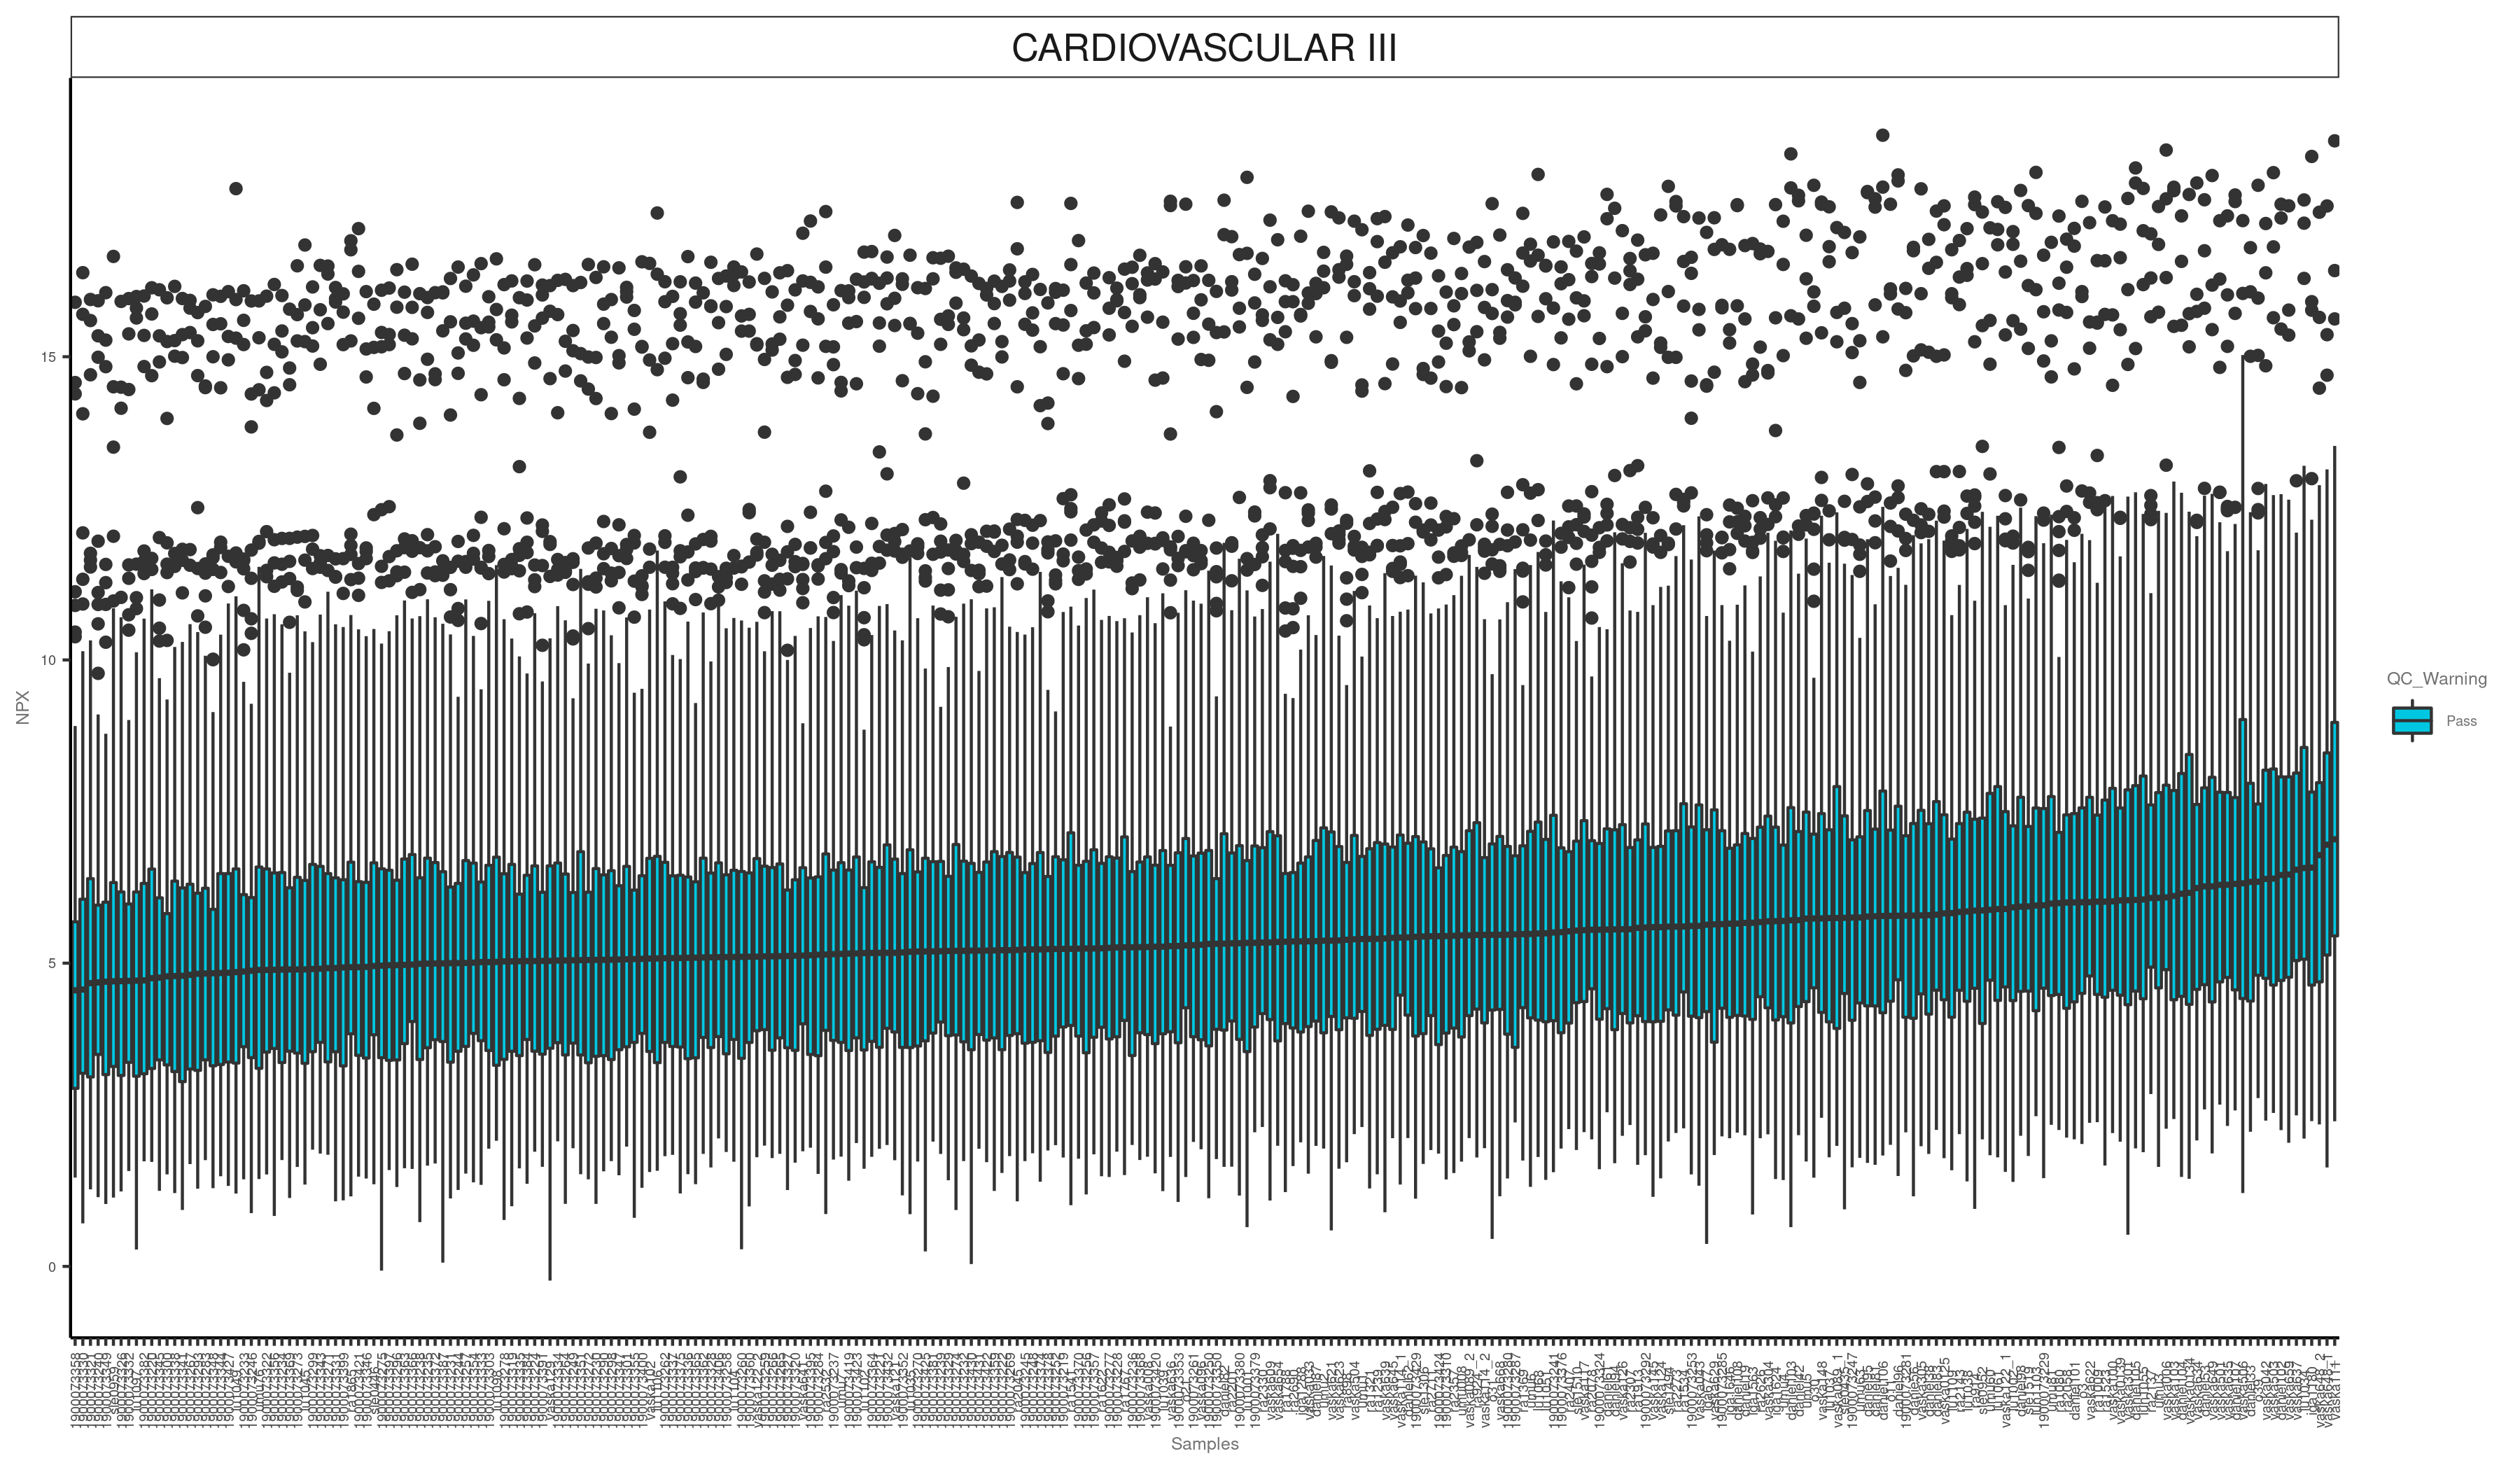
\includegraphics[width=0.49\linewidth,height=0.49\textheight]{../Results/Plasma/QC/plasma_CVIII_dist} }\subfloat[Inflammation\label{fig:plDistrBox-2}]{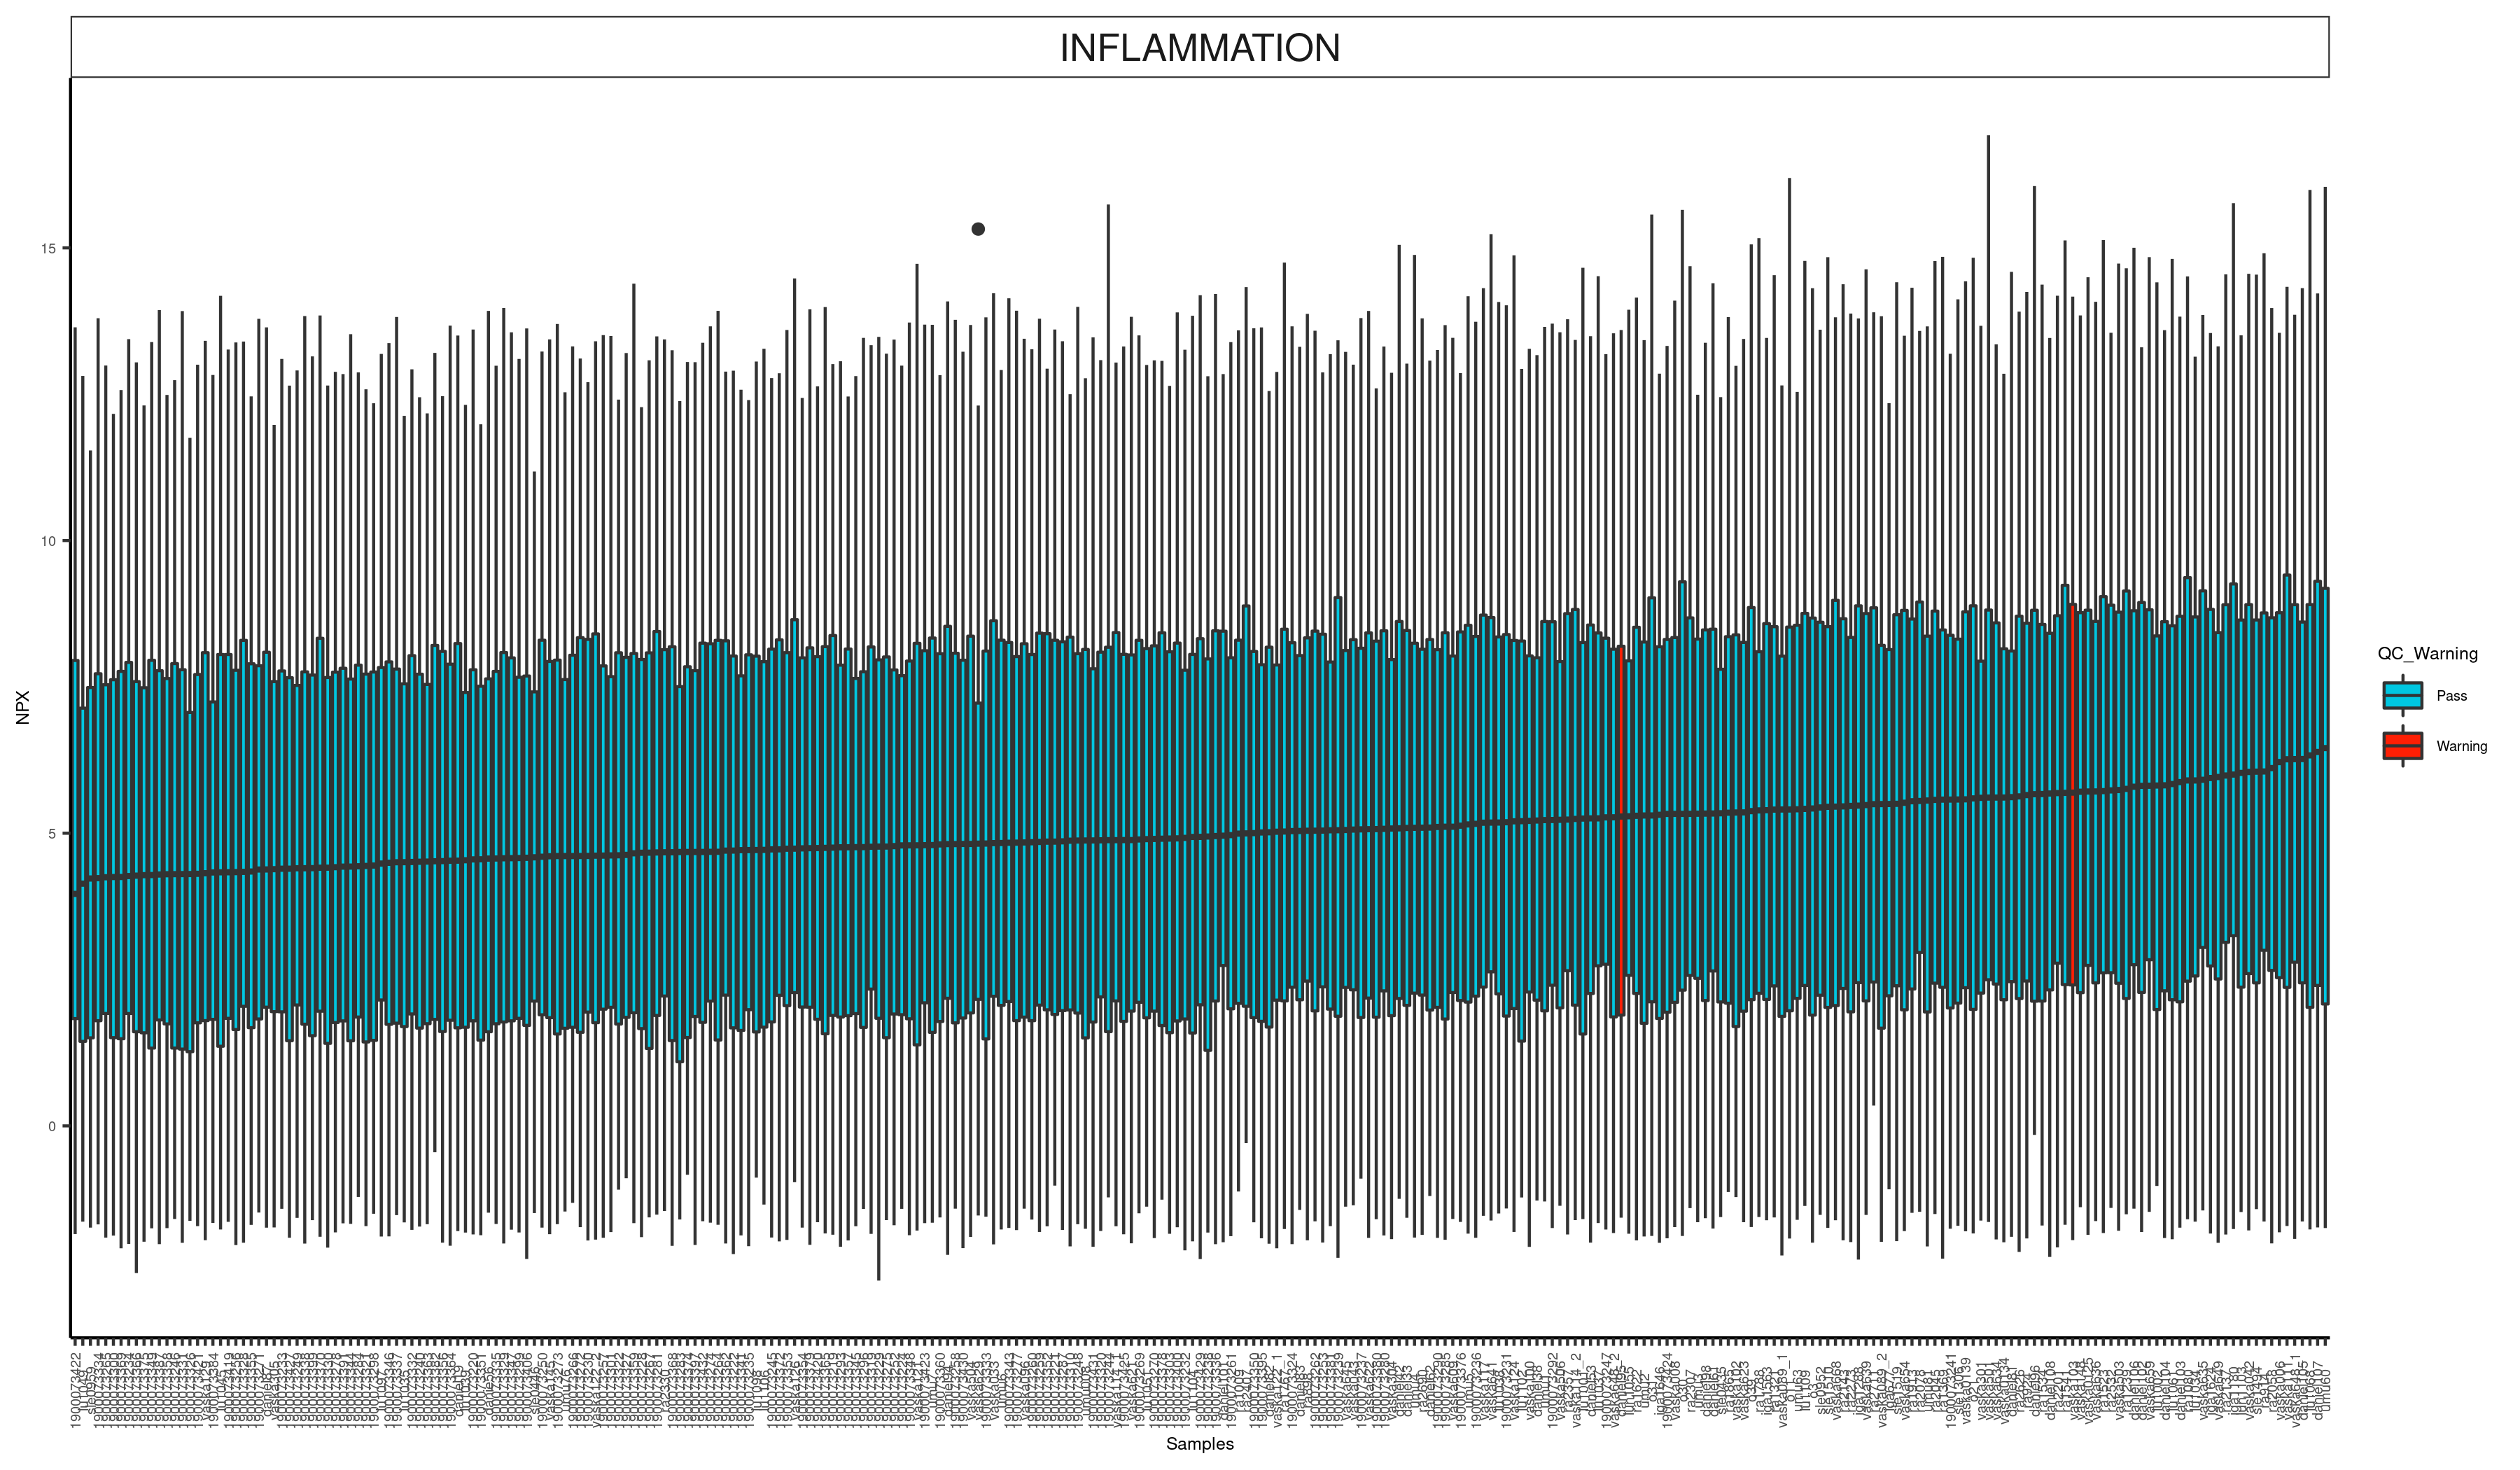
\includegraphics[width=0.49\linewidth,height=0.49\textheight]{../Results/Plasma/QC/plasma_INF_dist} }

}

\caption{Boxplots of NPX distribution per sample by panel ordered by median NPX value}\label{fig:plDistrBox}
\end{figure}

The distribution plot can get difficult to read when there are a large number
of samples or many panels. Plotting the interquartile range (IQR) vs the median
shows an alternative view on the data distributions (Figure \ref{fig:plIQR}).
Most samples cluster together, some samples have a slightly more extreme IQR.
Even though two samples are marked with QC warnings, their data distributions
(and PCA plot - data not shown) look ok. According to the Olink data analysis
tutorial, this means the samples can be kept for downstream analysis so they
were retained for further analysis.

\begin{figure}

{\centering 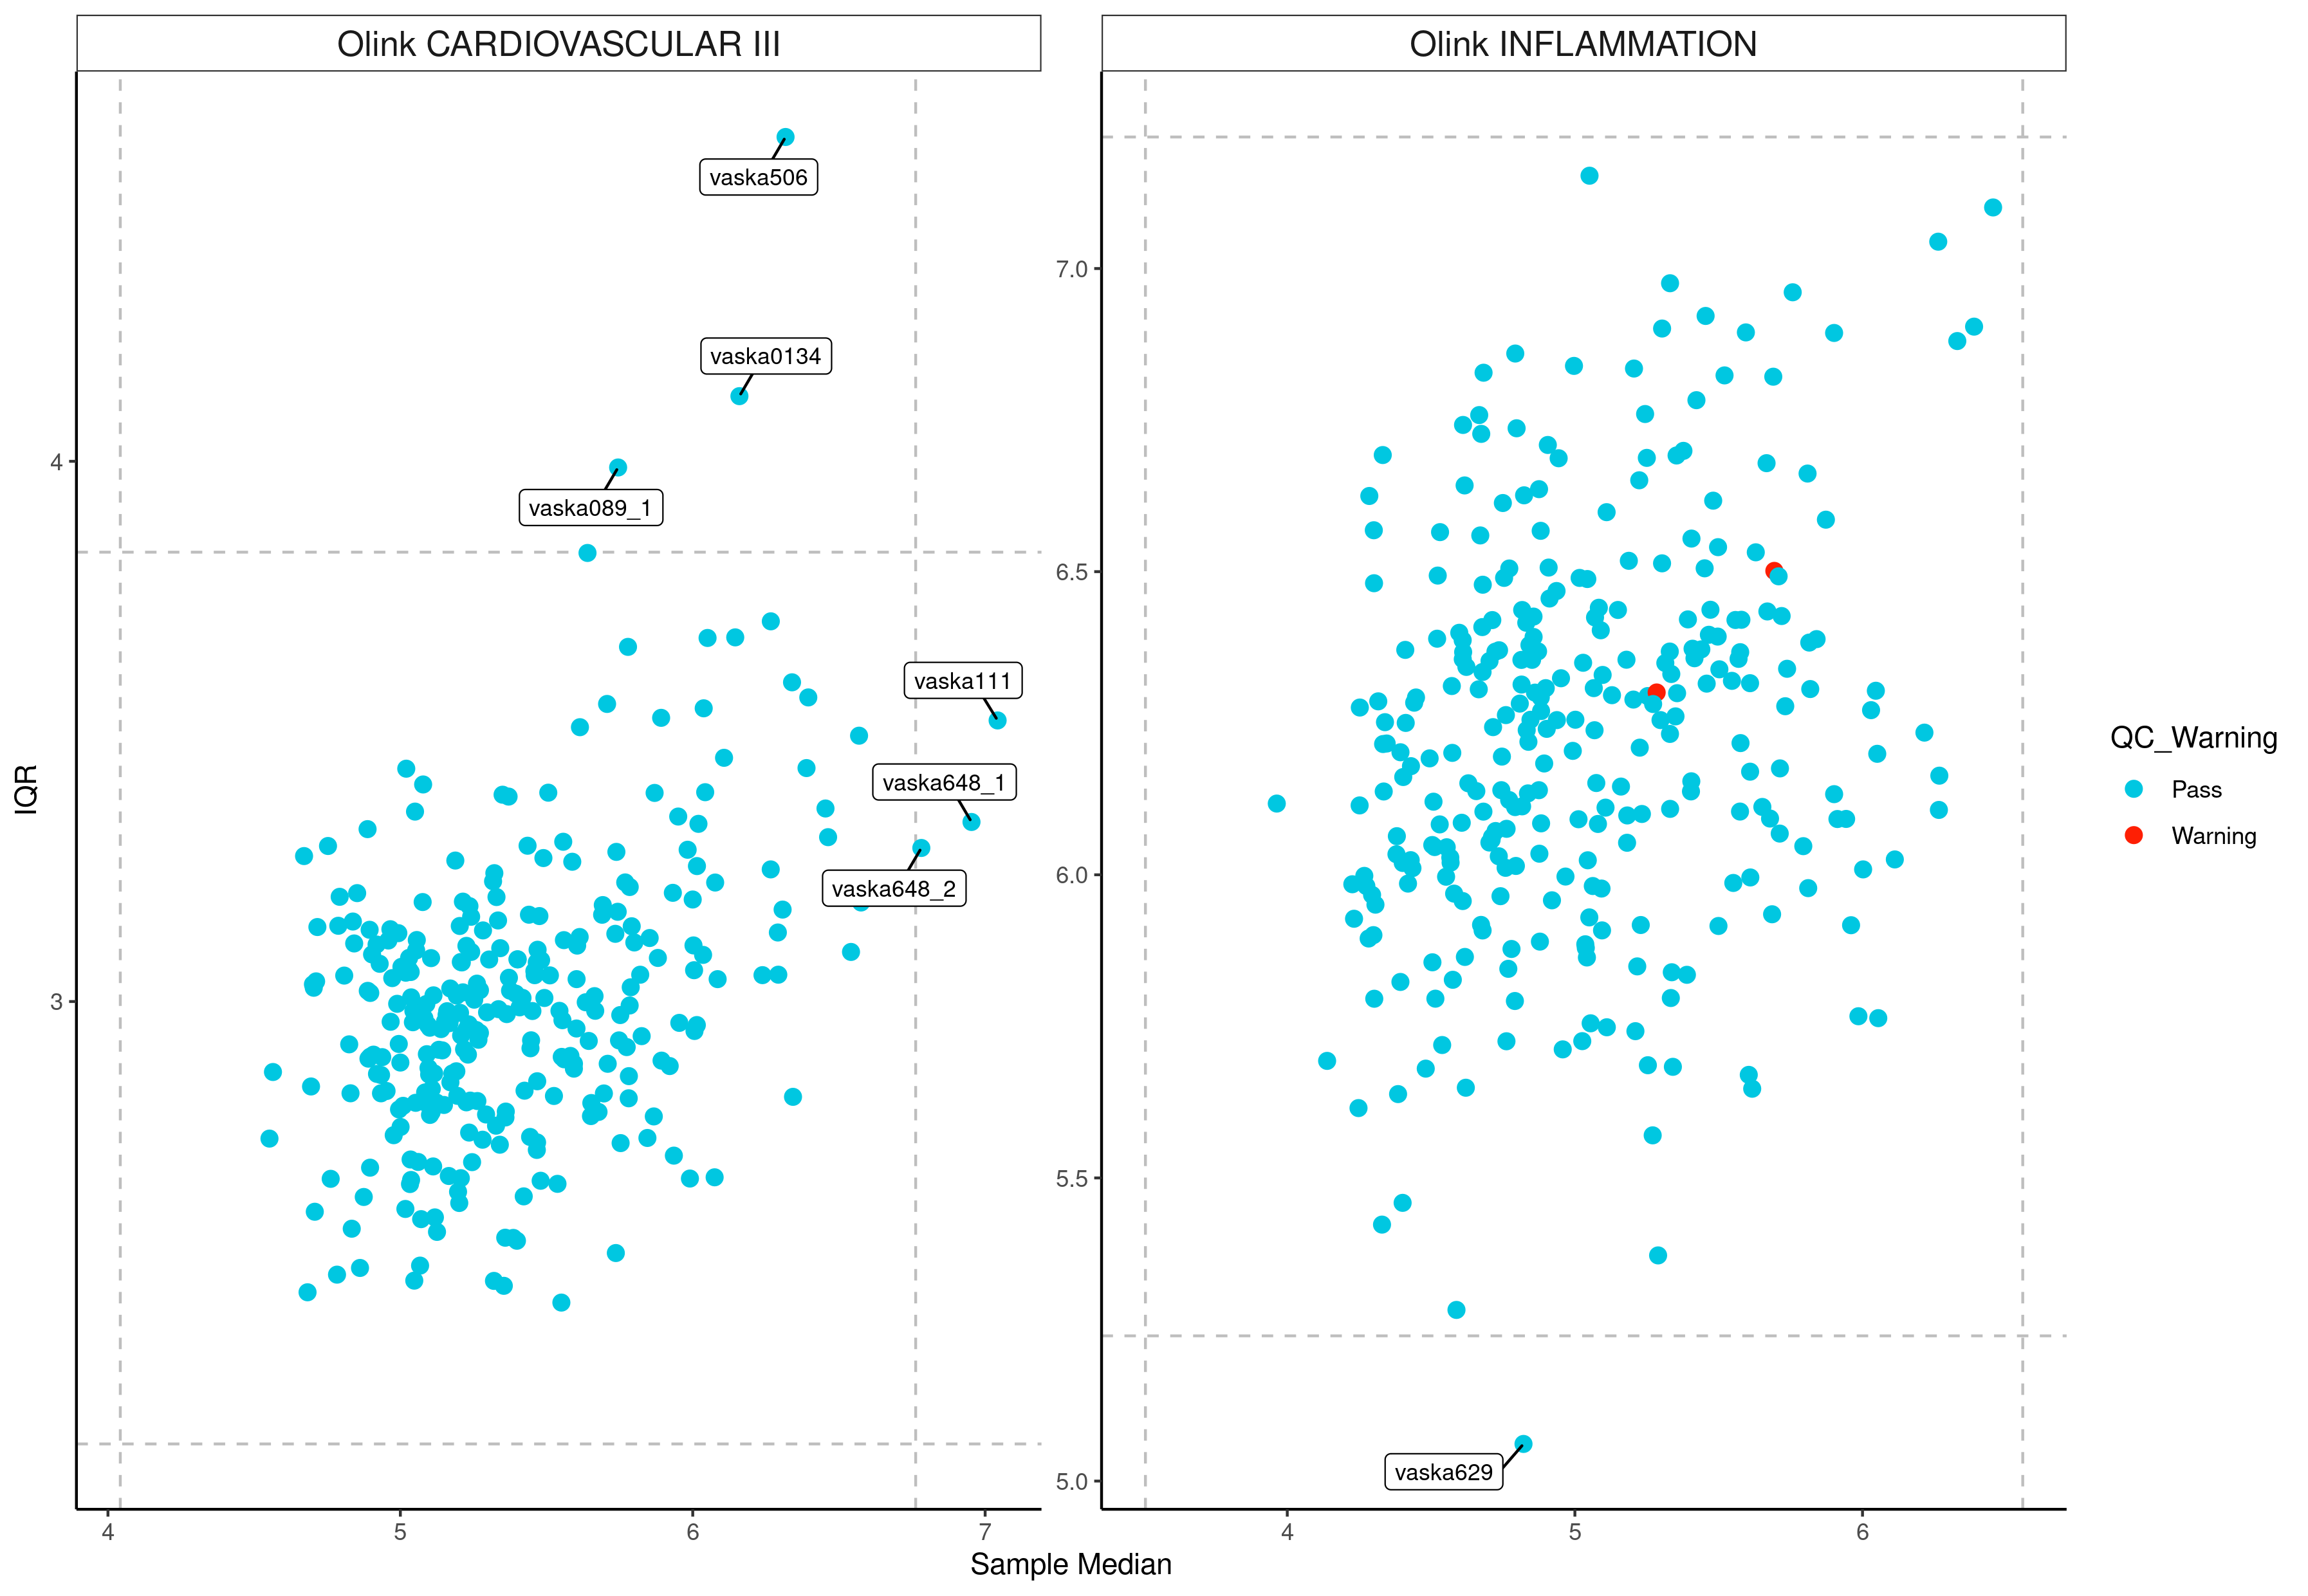
\includegraphics[width=1\linewidth]{../Results/Plasma/QC/plasma_qc} 

}

\caption{Interquartile range versus median per sample by panel ordered by median NPX value. Dashed lines indicate 3 standard deviations from the median or IQR mean.}\label{fig:plIQR}
\end{figure}

\hypertarget{pca}{%
\section{PCA}\label{pca}}

Using \href{http://setosa.io/ev/principal-component-analysis}{Principal Component
Analysis} (PCA), we examine
the structure of the data by projecting the samples on a two-dimensional graph
using the two first principal components (PC). These components are linear
combinations of the proteins that explain the most variation between those
samples. These plots can be used to examine the samples for outliers, sample
swaps, batch effects and other relationships. When normalization successfully
removed technical or batch artefacts, the relative distances should be
biologically interpretable. A plot of PC1 vs PC2 using the 100 most variable
proteins and colored by their biological/experimental group is shown in Figure
\ref{fig:plPCA}. Each point corresponds to a sample plotted by PC1 and PC2.
The different experimental groups do seem to differ, especially along PC1.
Also, the healthy control samples seem to cluster more together than the active
or other control samples.

\begin{figure}

{\centering 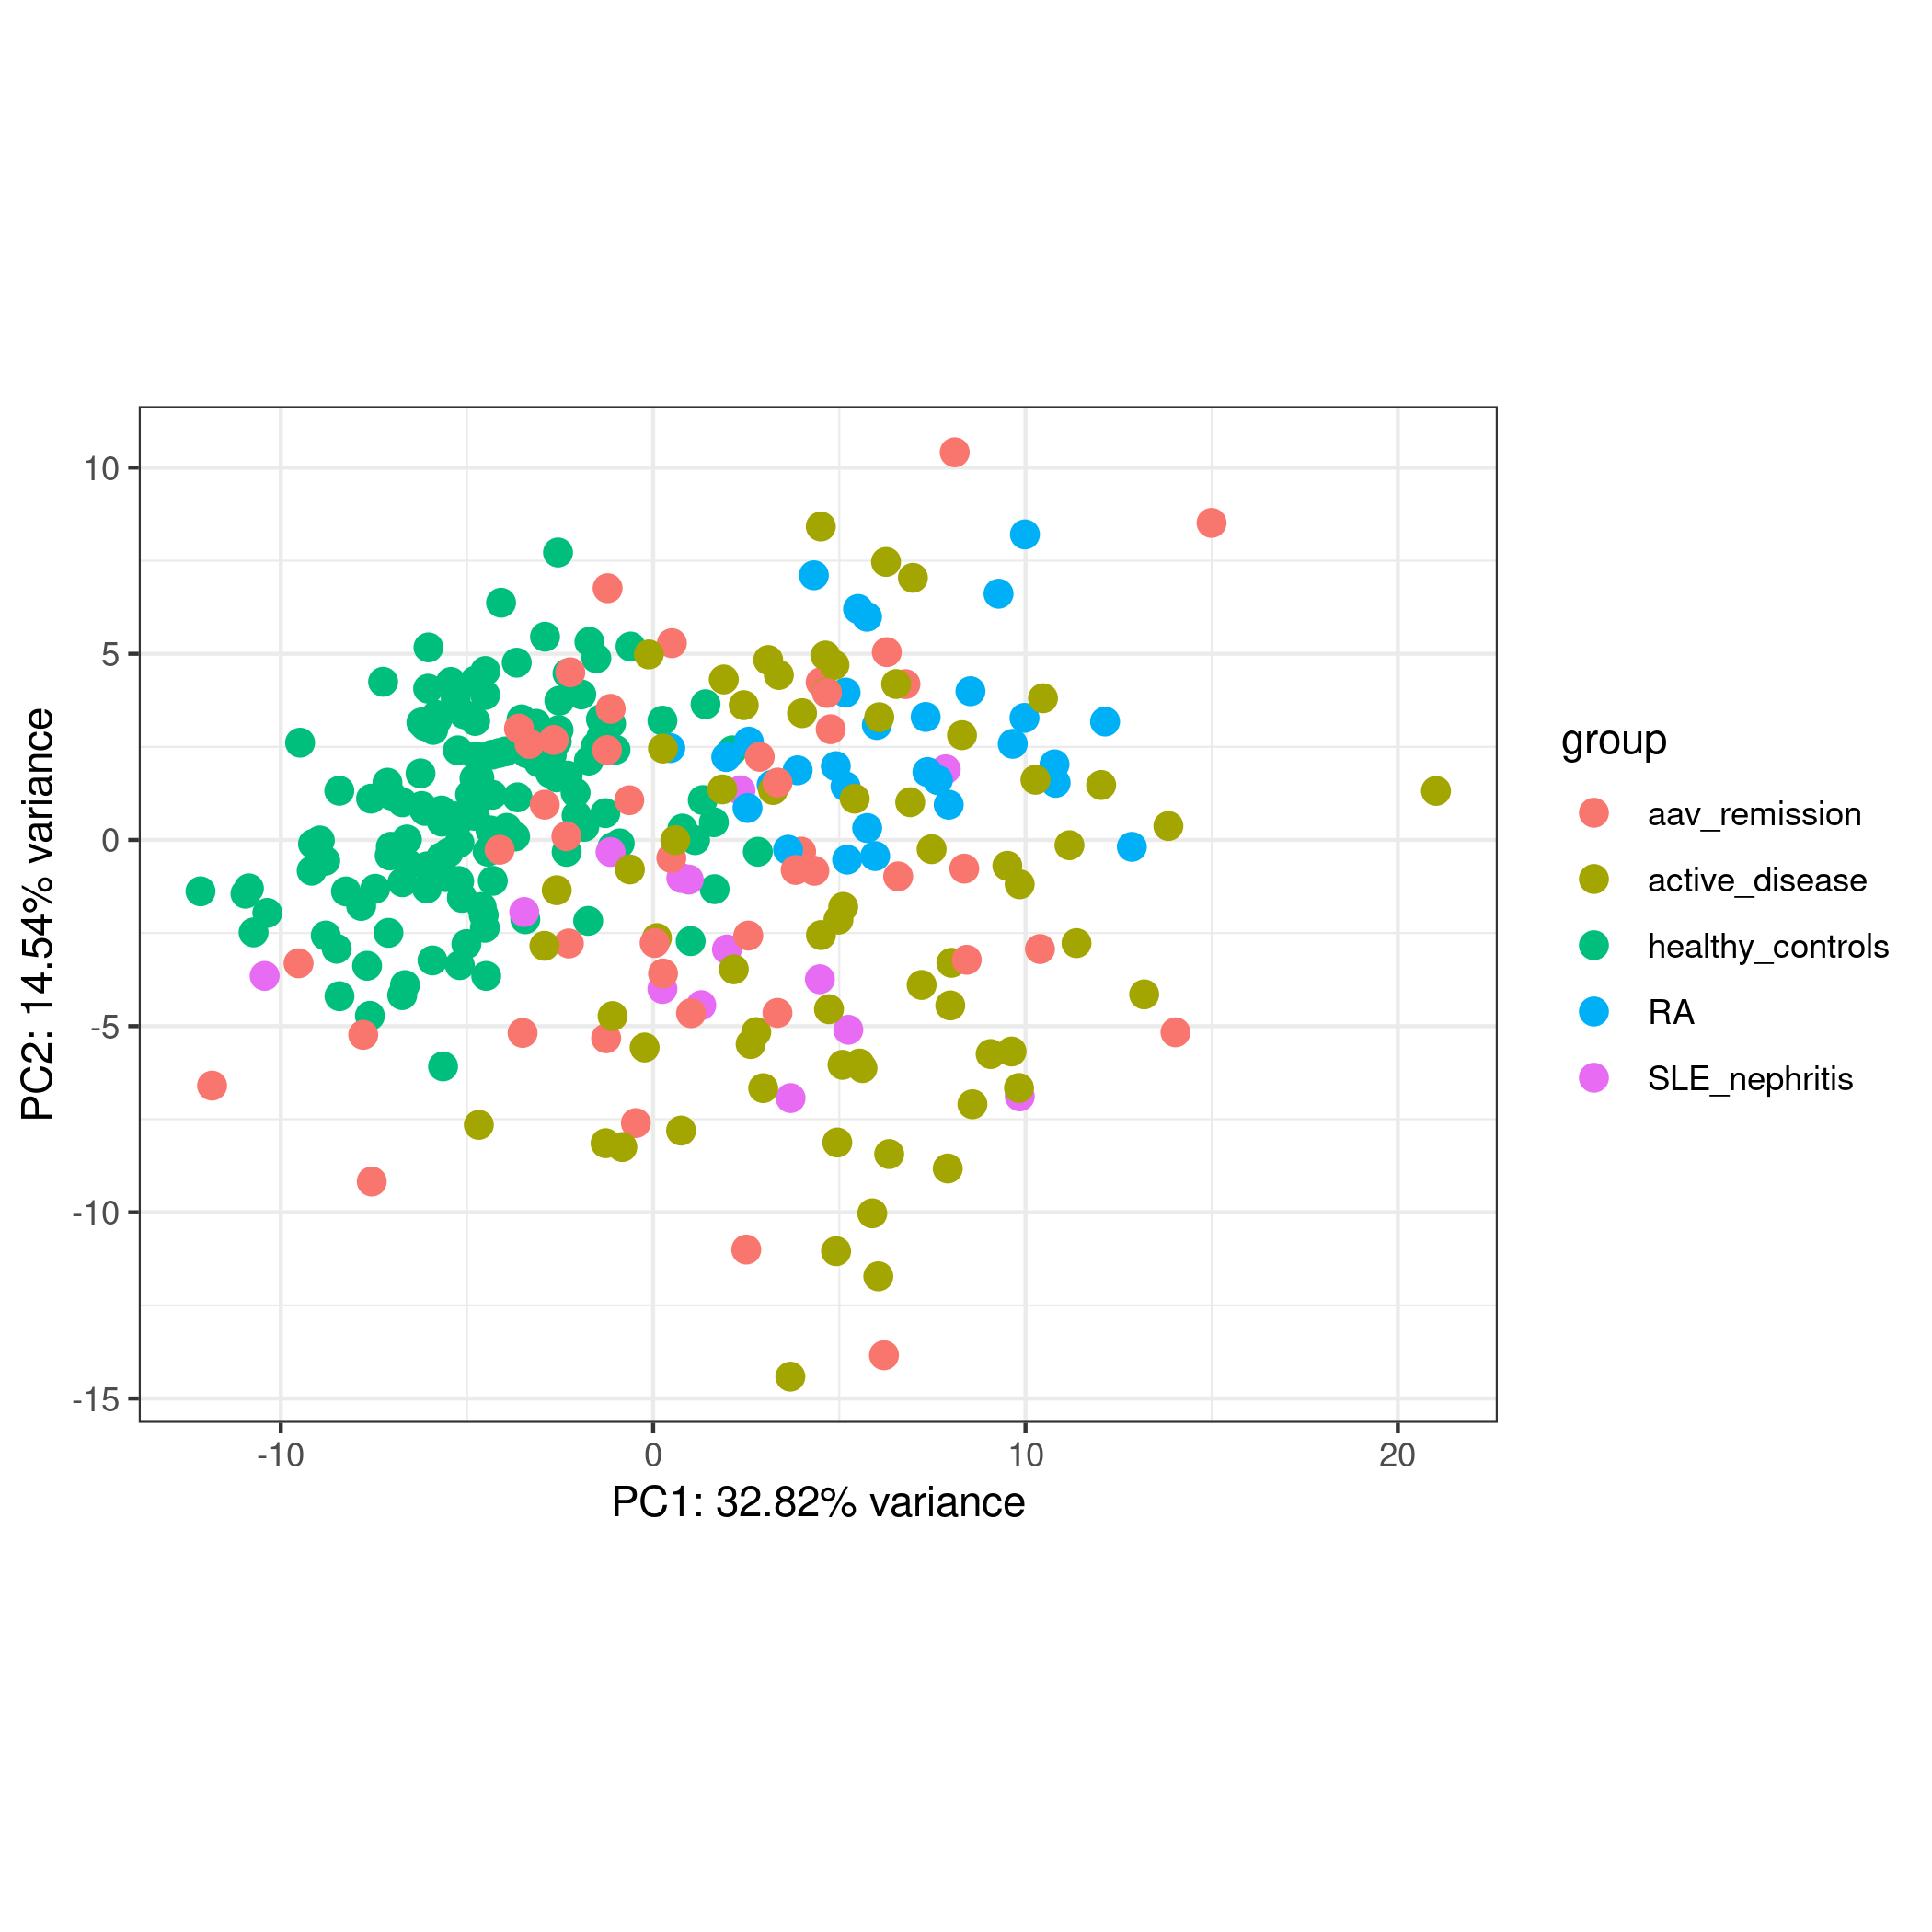
\includegraphics[width=1\linewidth]{../Results/Plasma/QC/plasma_pca_100} 

}

\caption{PCA plot of all plasma samples coloured by biological group.}\label{fig:plPCA}
\end{figure}

In the QC folder you will find additionally a PCA plot of PC1 vs PC3, a
screeplot showing the explained variation per PC and a barplot showing the top
and bottom genes contributing to the variation on PC1.

\hypertarget{differential-expression}{%
\chapter{Differential Expression}\label{differential-expression}}

To compare the different sample groups against each other we applied two
complementary statistical techniques: univariate ANOVA and multivariate pls-da.
ANOVA (followed by a post-hoc analysis) has as a benefit that it is fairly
straightforward to interpret the results and will return the most differential expressed
proteins and how much they differ between the groups. The multivariate pls-da
technique is harder to interpret but can take correlations among the proteins
into account and might therefore result in a more robust set of proteins to
serve as markers distinguishing the groups. It will however not return an
estimate of the different expression among the groups, but rather a measure of
how important a certain protein is in separating the subgroups.

Following comparisons were looked at:

\begin{itemize}
\tightlist
\item
  aav\_remission vs active\_disease
\item
  aav\_remission vs healthy\_controls
\item
  aav\_remission vs RA
\item
  aav\_remission vs SLE\_nephritis
\item
  active\_disease vs healthy\_controls
\item
  active\_disease vs RA
\item
  active\_disease vs SLE\_nephritis
\item
  healthy\_controls vs RA
\item
  healthy\_controls vs SLE\_nephritis
\item
  MPA vs GPA
\item
  MPO\_pos vs PR3\_pos
\item
  RA vs SLE\_nephritis
\end{itemize}

All results for each comparison are collected in either \textbf{/Plasma/Comparisons}
or \textbf{/Serum/Comparisons}.

To keep the size of this report manageable, the results shown here are limited to the
active\_disease vs healthy\_control comparison in Plasma. The results for all
other comparisons are found in the appropriate folder of the Results
directory.

\hypertarget{univariate-analysis}{%
\section{Univariate Analysis}\label{univariate-analysis}}

The ANOVA F-test will be used to assess whether the protein expression varies
significantly across the different sample groups, one protein at a time. If
this is the case, a post-hoc test will look at all pairwise group comparisons
to determine which comparisons are in fact resulting in the differential
expression. An adjusted p-value (Tukey) will be calculated per protein.

For the ANOVA analysis, a correction for the patient covariates \emph{age} and
\emph{ckd\_epi} level was applied to the linear model.

Results for the per-protein analysis is collected in \textbf{Results/Plasma/Comparisons/\{comparison\}\}/Univariate/} and \textbf{Results/Serum/Comparisons/\{comparison\}\}/Univariate/}.

\hypertarget{protein-level}{%
\subsection{Protein-level}\label{protein-level}}

A volcano plot of the post-hoc results is made for each comparison. In these type of plots, proteins in the left or right upper quadrant are the most significantly differentially expressed. The volcano plot for active\_disease vs healthy\_control is shown in Figure \ref{fig:glplots} (Left). In addition, a heatmap of proteins with a adjusted p-value \textless{} 0.05 is produced. In this visualization, samples are clustered according to the expression of these significant proteins (see Figure \ref{fig:glplots} (Right)).

\begin{figure}

{\centering 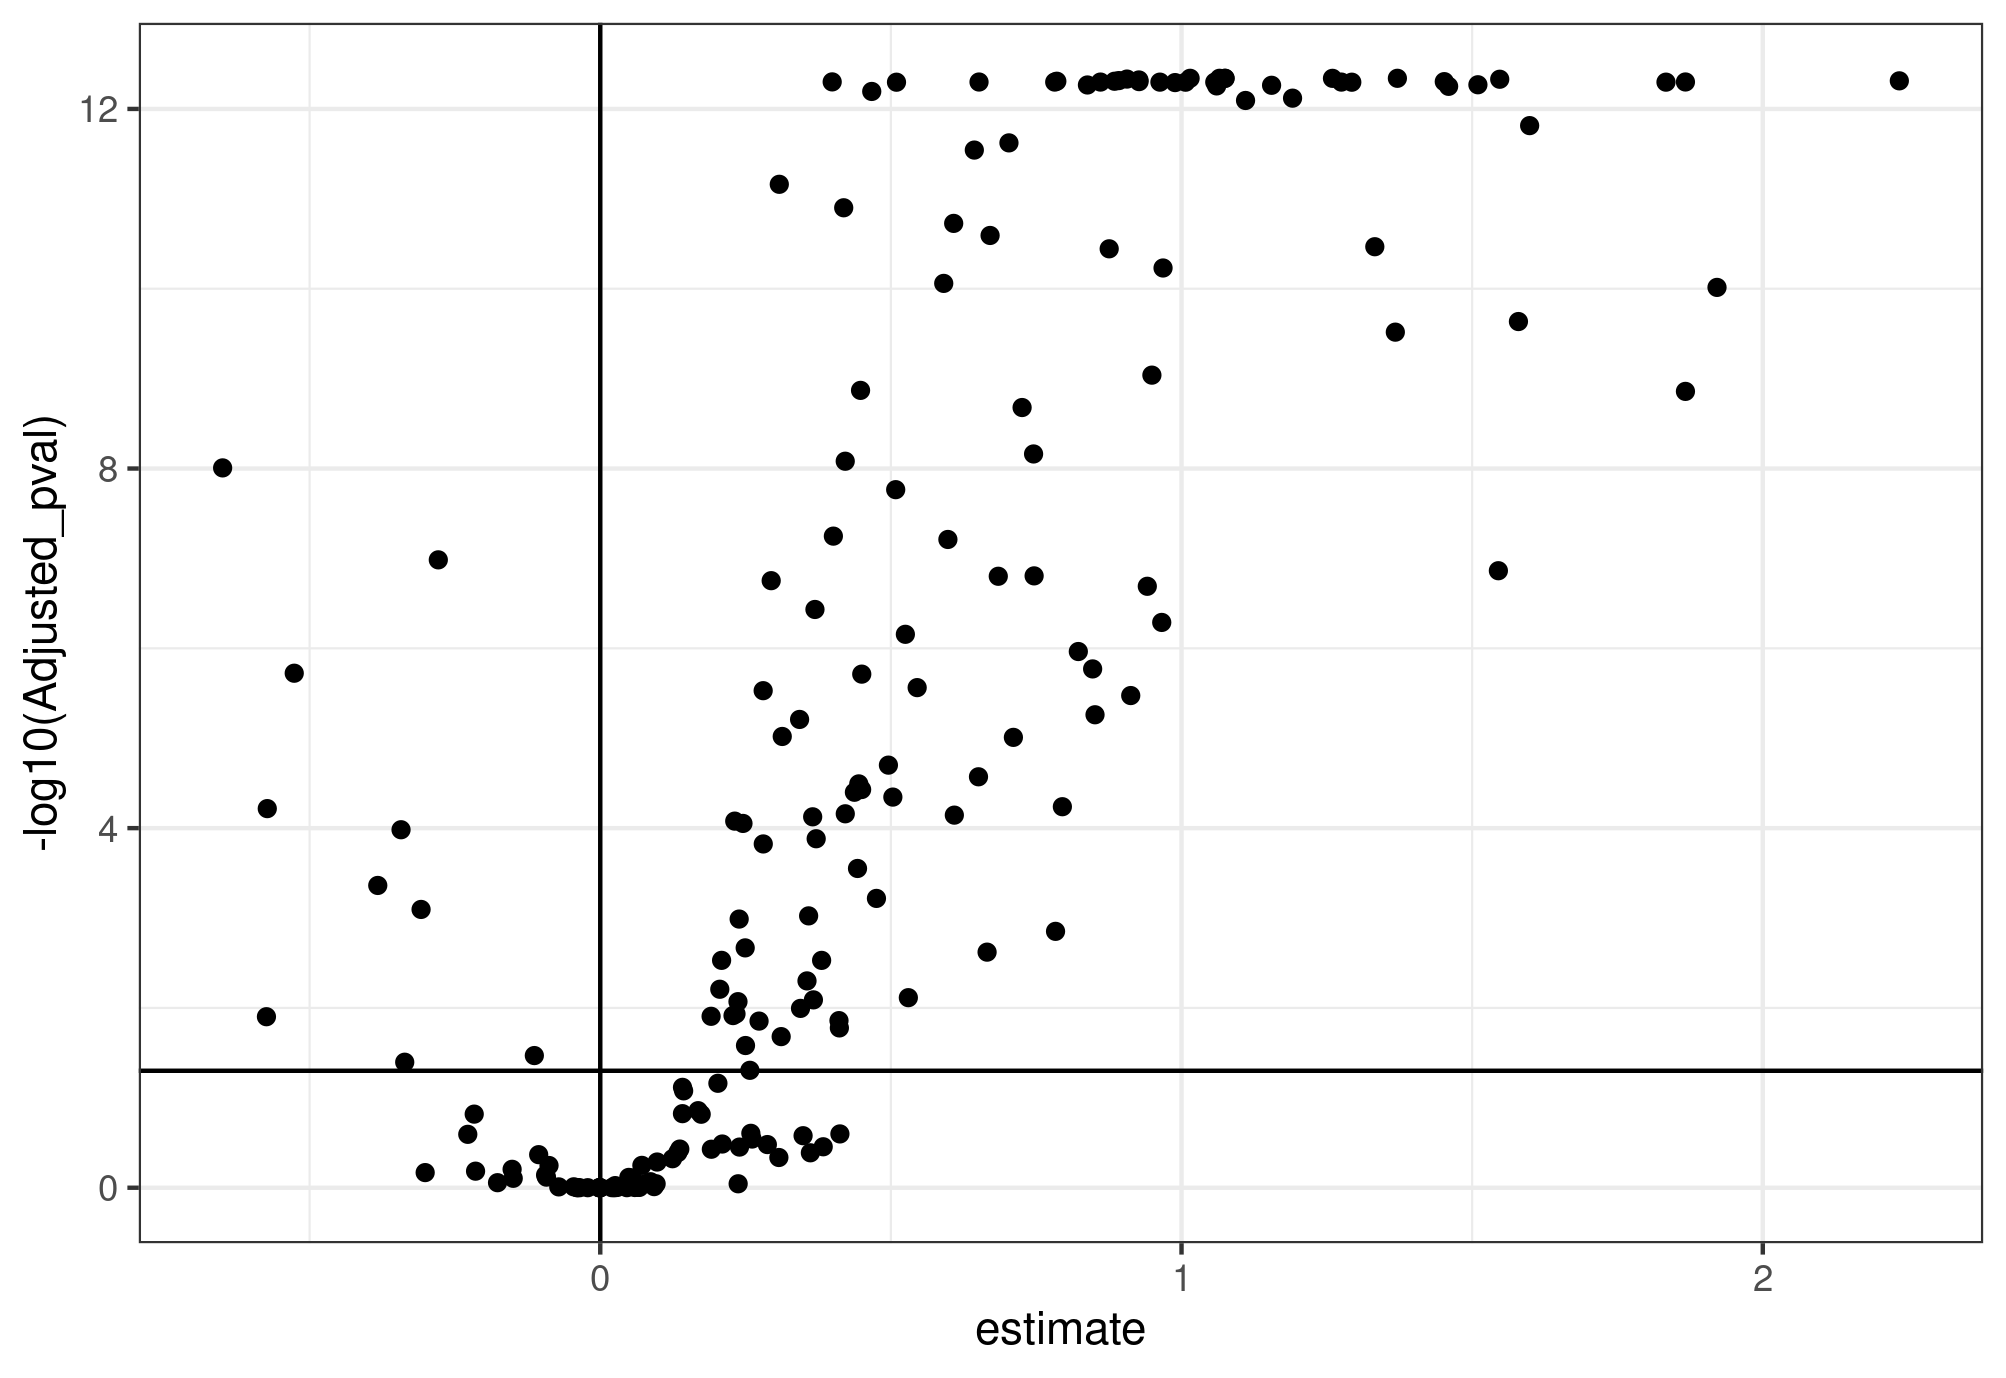
\includegraphics[width=0.49\linewidth]{../Results/Plasma/Comparisons/active_disease_vs_healthy_controls/Univariate/active_disease_vs_healthy_controls_volcano_anova_posthoc} 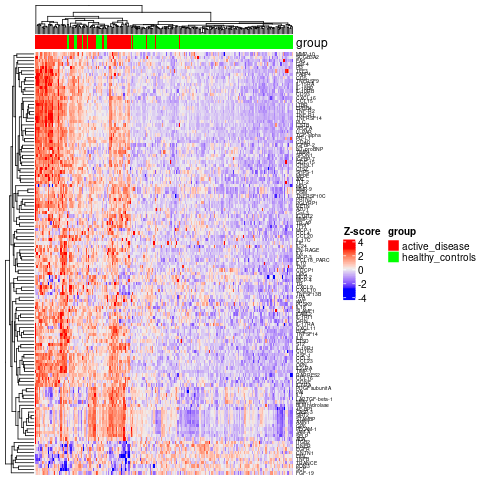
\includegraphics[width=0.49\linewidth]{../Results/Plasma/Comparisons/active_disease_vs_healthy_controls/Univariate/Heatmap_Sig_Prots_Prots} 

}

\caption{Two visualizations of the gene-level differential expression. Volcano plot (Left) Heatmap of the significant proteins (Right).}\label{fig:glplots}
\end{figure}

The top 15 of most significantly regulated proteins (ranked by adjusted p-value) of active\_disease versus healthy\_controls is shown in \ref{fig:top15}. The ``estimate'' column can be considered as a log2 fold change, where a higher estimate means a higher expression in active\_disease samples (i.e.~a difference of 1 indicates a doubled expression).

\begin{figure}

{\centering 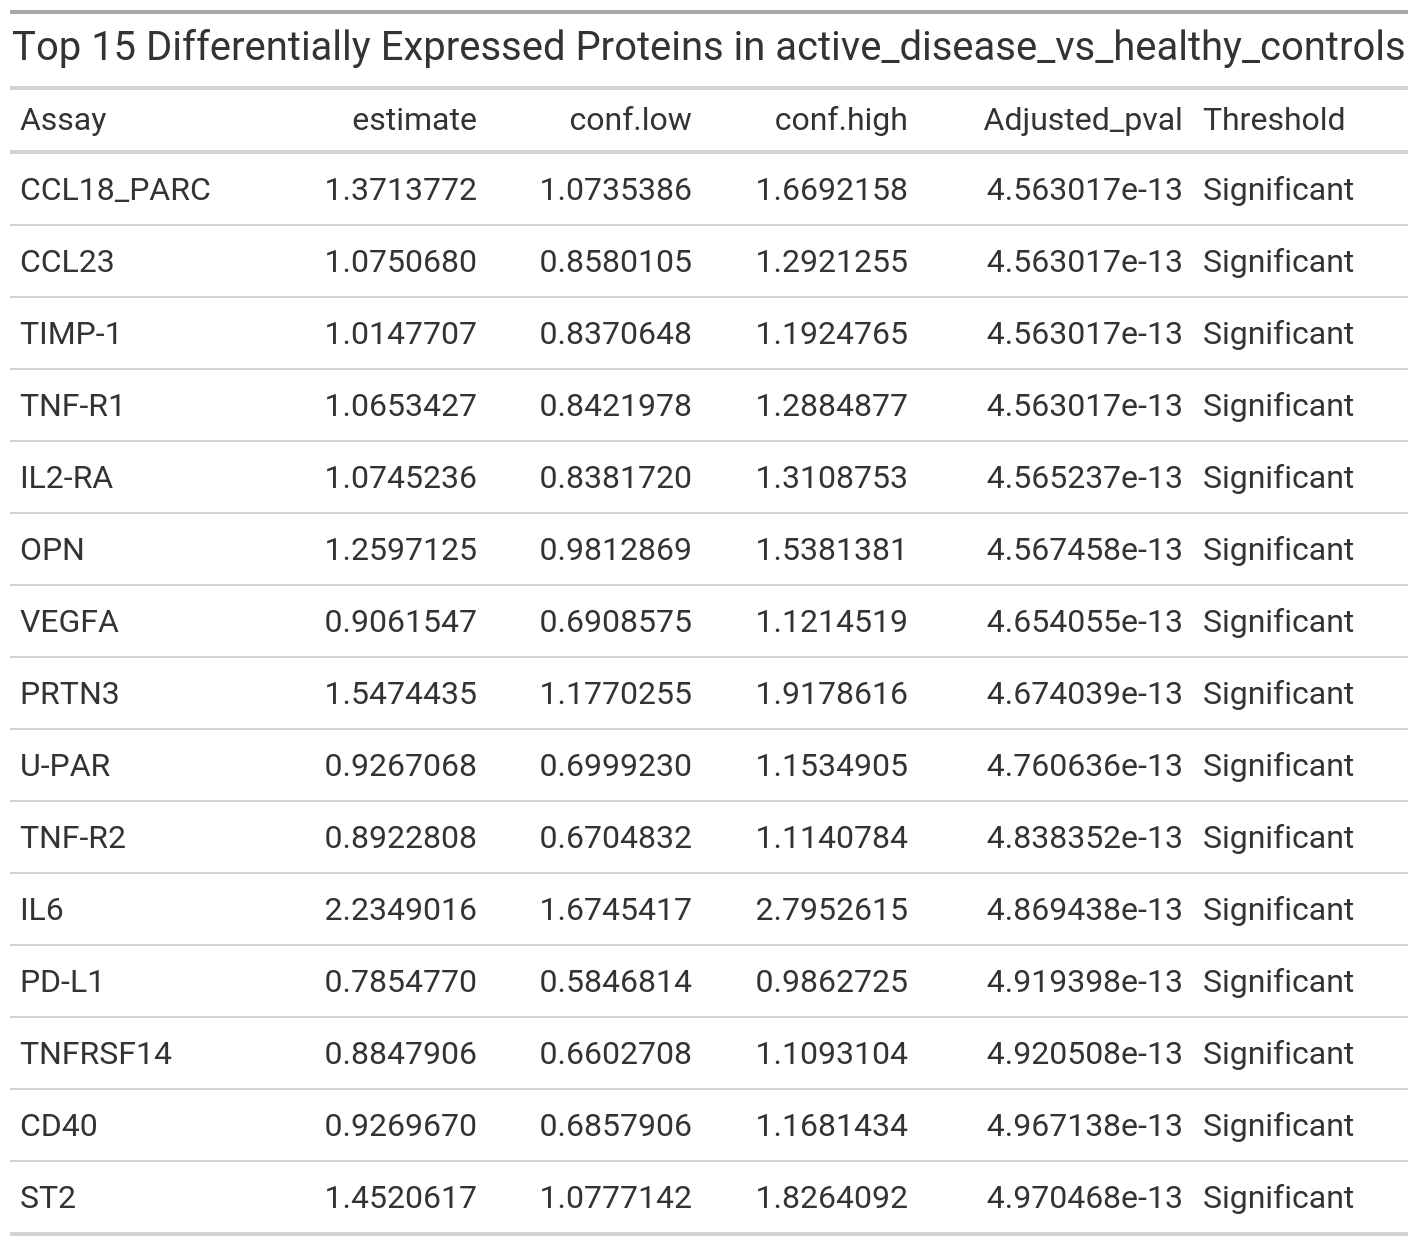
\includegraphics[width=0.75\linewidth]{../Results/Plasma/Comparisons/active_disease_vs_healthy_controls/Univariate/active_disease_vs_healthy_controls_Top15_table} 

}

\caption{Table of 15 most DE proteins}\label{fig:top15}
\end{figure}

A full list of results for all proteins can be found in \textbf{/Results/Plasma/Comparisons/active\_disease\_vs\_healthy\_controls/Univariate/active\_disease\_vs\_healthy\_controls\_anova\_posthoc\_results.xlsx}.

\hypertarget{gsea}{%
\subsection{GSEA}\label{gsea}}

Each univariate comparison folder (e.g.~\textbf{Results/Plasma/Comparisons/active\_disease\_vs\_healthy\_controls/Univariate/}) contains a \textbf{GSEA/} folder that contains the output of a gene set enrichment analysis. GSEA uses a statistical metric comparing two conditions to rank all genes (for example according to Log2FoldChange) and applies a weighted Kolmogorov--Smirnov (KS) statistic to calculate an Enrichment Score (ES).

Calculation of the Enrichment Score:

\begin{itemize}
\tightlist
\item
  Rank genes by a statistic (e.g.~log2FoldChange)
\item
  Compute cumulative sum over ranked genes:

  \begin{itemize}
  \tightlist
  \item
    Increase sum when gene in set, decrease it otherwise.
  \item
    Magnitude of increment depends on correlation of gene
    with phenotype.
  \end{itemize}
\item
  Record the maximum deviation from zero as the enrichment score (ES)
\end{itemize}

The ES and NES (ES normalized for set size) of a set are calculated by looking at where the statistics of genes belonging to a certain set can be found in the ranked gene list. A high (N)ES indicates these genes are found high up in the list. In other words, a high (N)ES value means that for the genes in this set there is - on average - a shift towards a higher expression. The significance of each (N)ES is calculated permuting the sets and recomputing ES, getting a null distribution for the ES. A multiple comparison correction is also performed on the p values. More info on the GSEA algorithm can be found \href{https://bioinformatics.mdanderson.org/MicroarrayCourse/Lectures09/gsea1_bw.png}{here}.

In this project we used the ``estimate'' as the statistic to rank the genes (equivalent to log2FoldChange). When it comes to the gene sets to be tested, a compendium of gene sets developed and maintained by the Bader Lab was used (called Human\_GOBP\_AllPathways\_no\_GO\_iea\_March\_01\_2021\_symbol.gmt; download \href{http://download.baderlab.org/EM_Genesets/March_01_2021/Human/symbol/Human_GOBP_AllPathways_no_GO_iea_March_01_2021_symbol.gmt}{here}). This gene set collection combines data from Gene Ontology (GO) with pathway data from MsigdB, Reactome, WikiPathways, \ldots{} for a total of around 18500 gene sets.

Each GSEA results folder contains a .xlsx file containing the full results and two different visualizations of the top terms (see Figure \ref{fig:gseaPlots}). These figures include a barplot of the gene sets with the 6 highest and 6 lowest NES values and an Enrichment map of the 20 gene sets with the highest absolute NES values. Enrichment maps organize gene sets into a network with edges connecting overlapping gene sets. In this way, mutually overlapping gene sets tend to cluster together, making it easier to identify functional modules.

\begin{figure}

{\centering 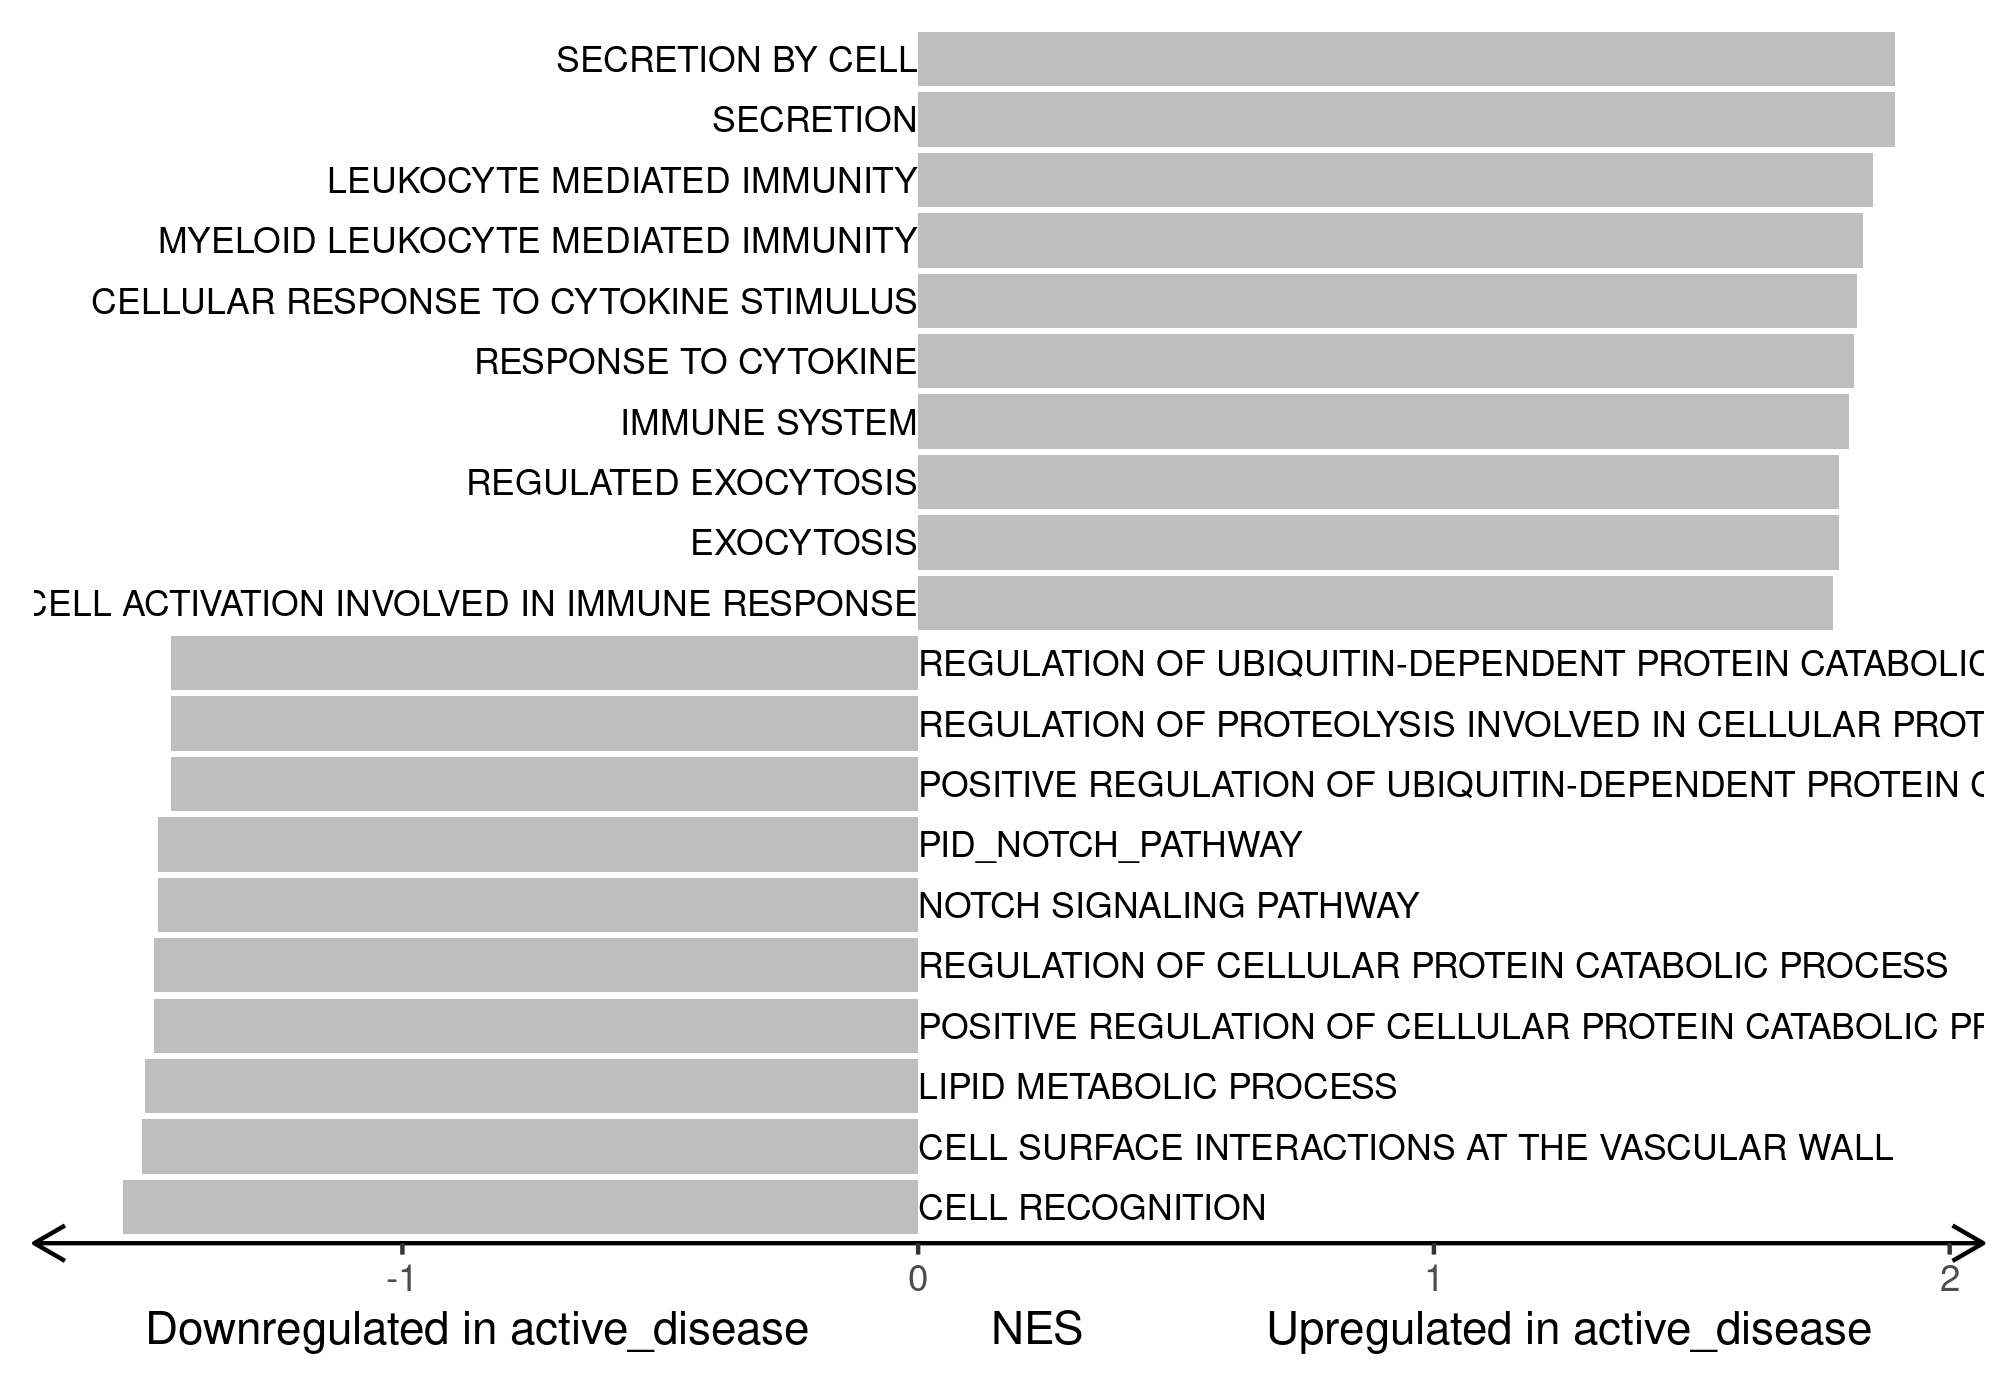
\includegraphics[width=0.49\linewidth]{../Results/Plasma/Comparisons/active_disease_vs_healthy_controls/Univariate/GSEA/active_disease_vs_healthy_controls_barplot} 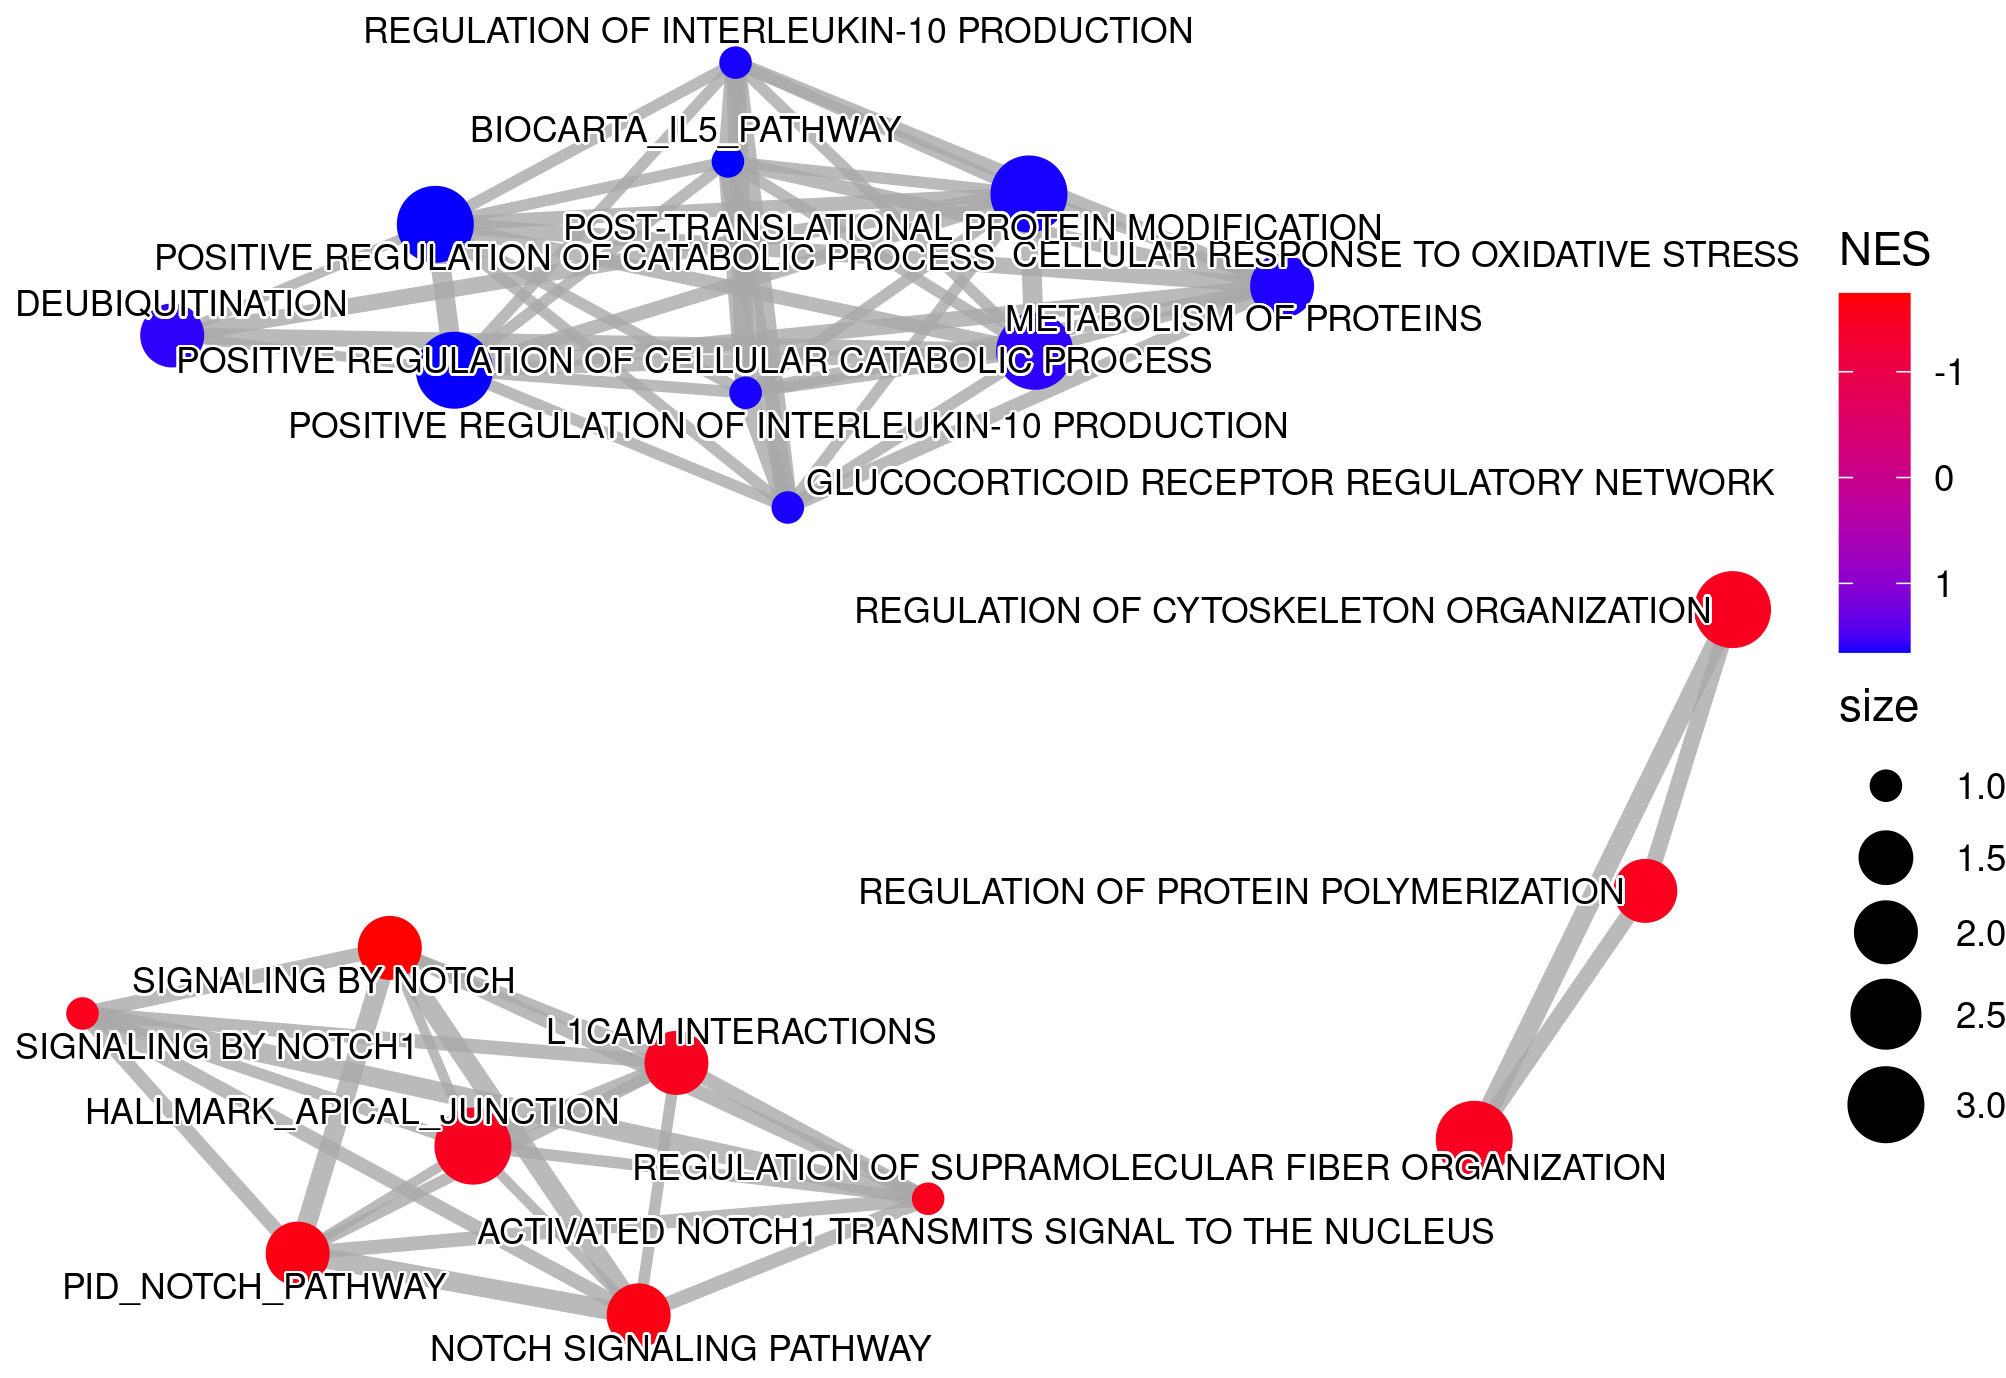
\includegraphics[width=0.49\linewidth]{../Results/Plasma/Comparisons/active_disease_vs_healthy_controls/Univariate/GSEA/active_disease_vs_healthy_controls_emap} 

}

\caption{Example of the different GSEA visualizations. (Left)  Barplot of the gene sets with the 10 highest and 10 lowest NES values. (Right) Enrichment map of the same gene sets.}\label{fig:gseaPlots}
\end{figure}

In addition, in the \textbf{GSEA\_PLOTS/} folder you can find a visualization of the location of the gene set genes in the ranked gene list and an ES calculation visualization (see Figure \ref{fig:gseaNes}).

\begin{figure}

{\centering 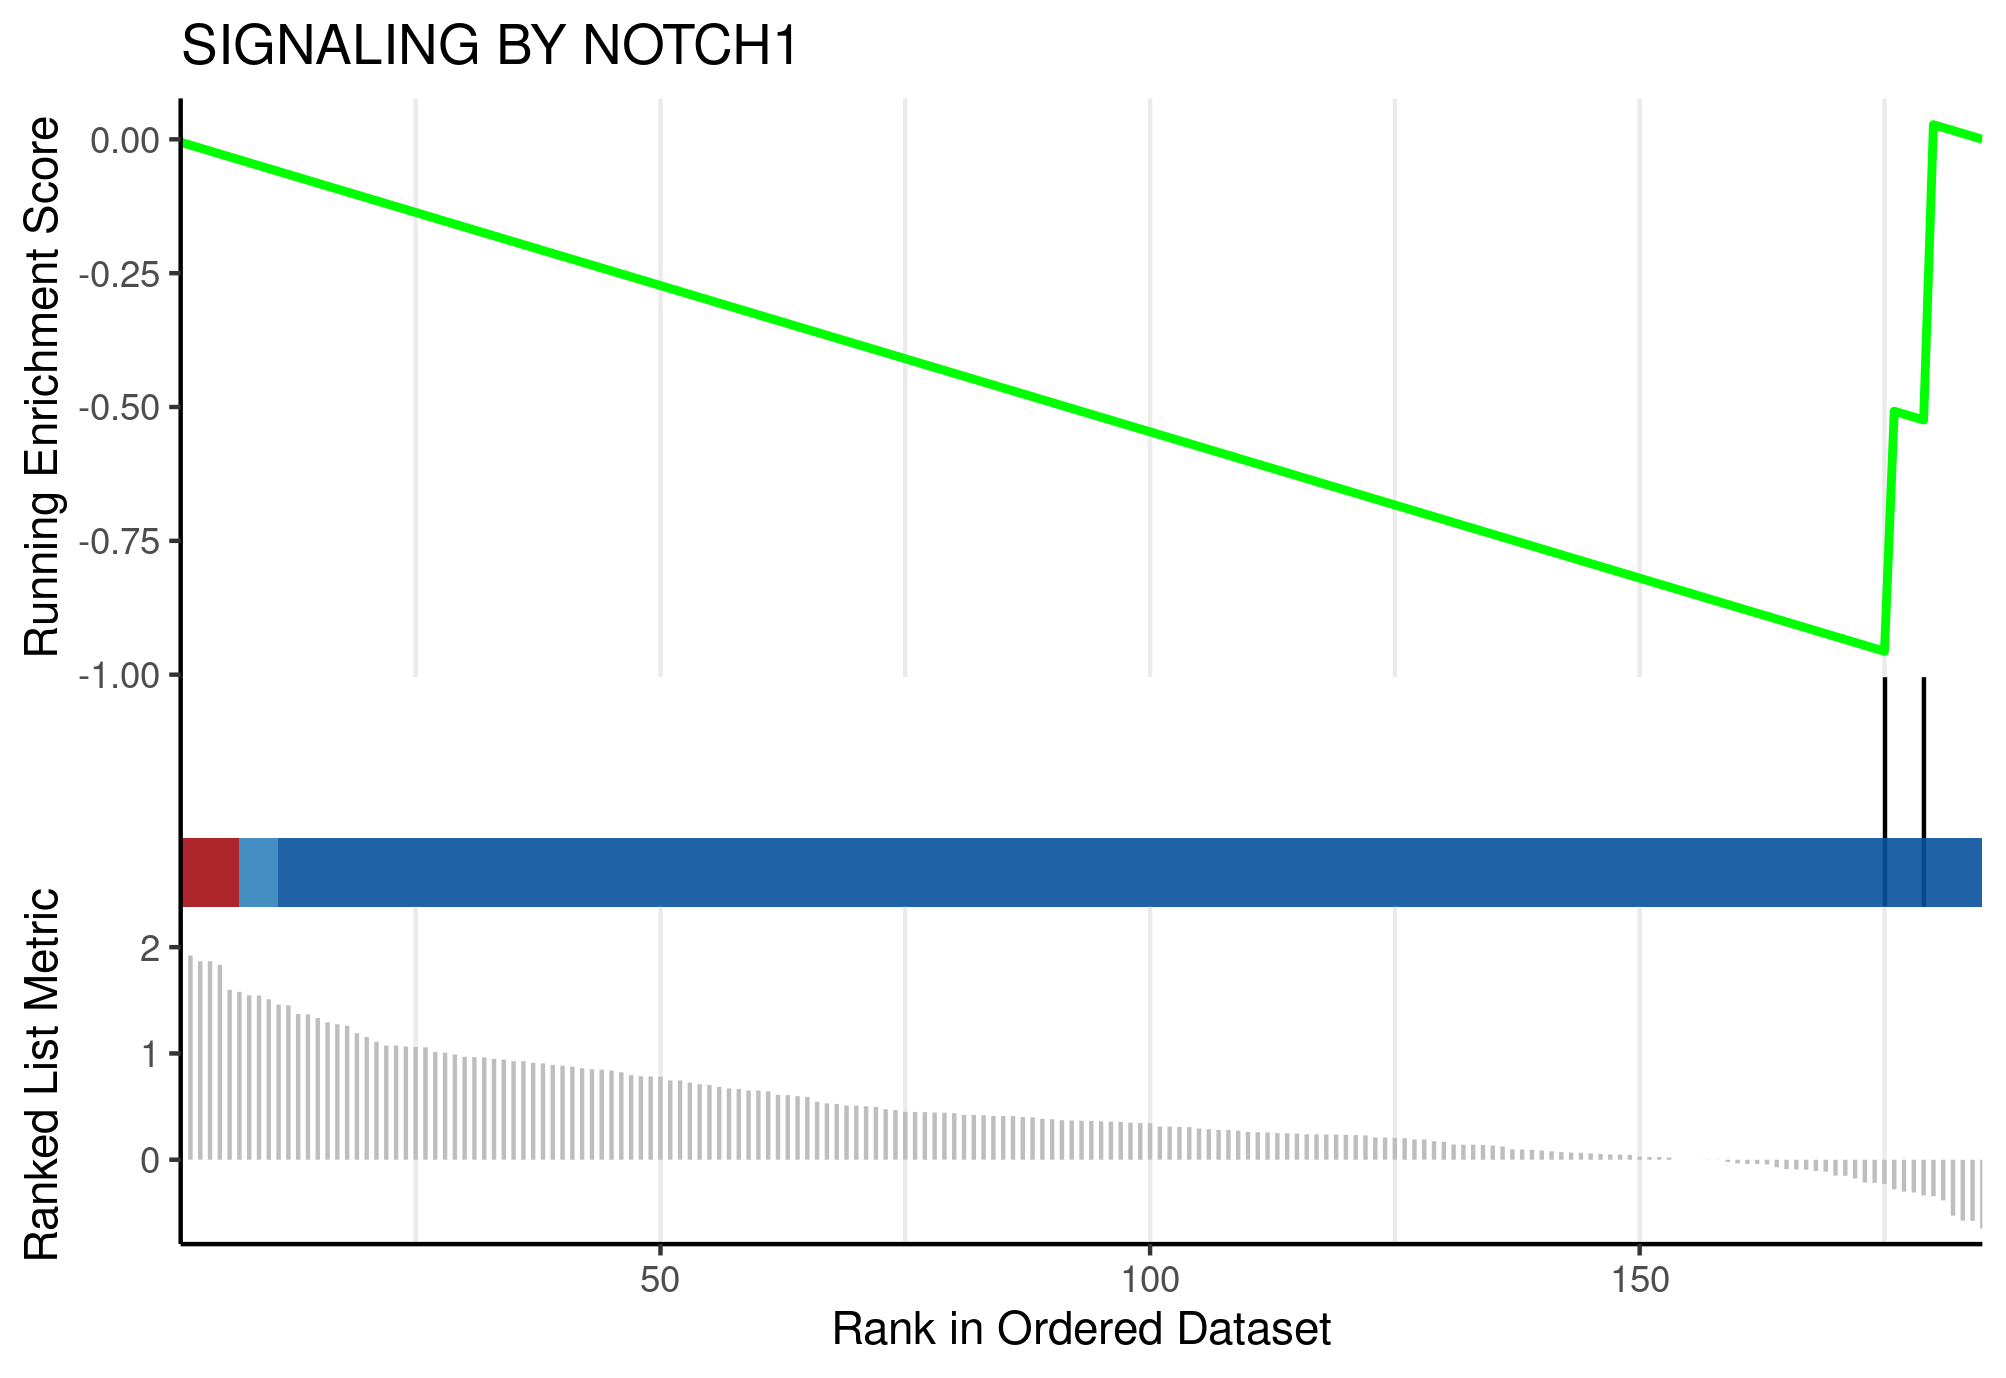
\includegraphics[width=0.49\linewidth]{../Results/Plasma/Comparisons/active_disease_vs_healthy_controls/Univariate/GSEA/GSEA_PLOTS/active_disease_vs_healthy_controls_gseaplot_SIGNALING_BY_NO} 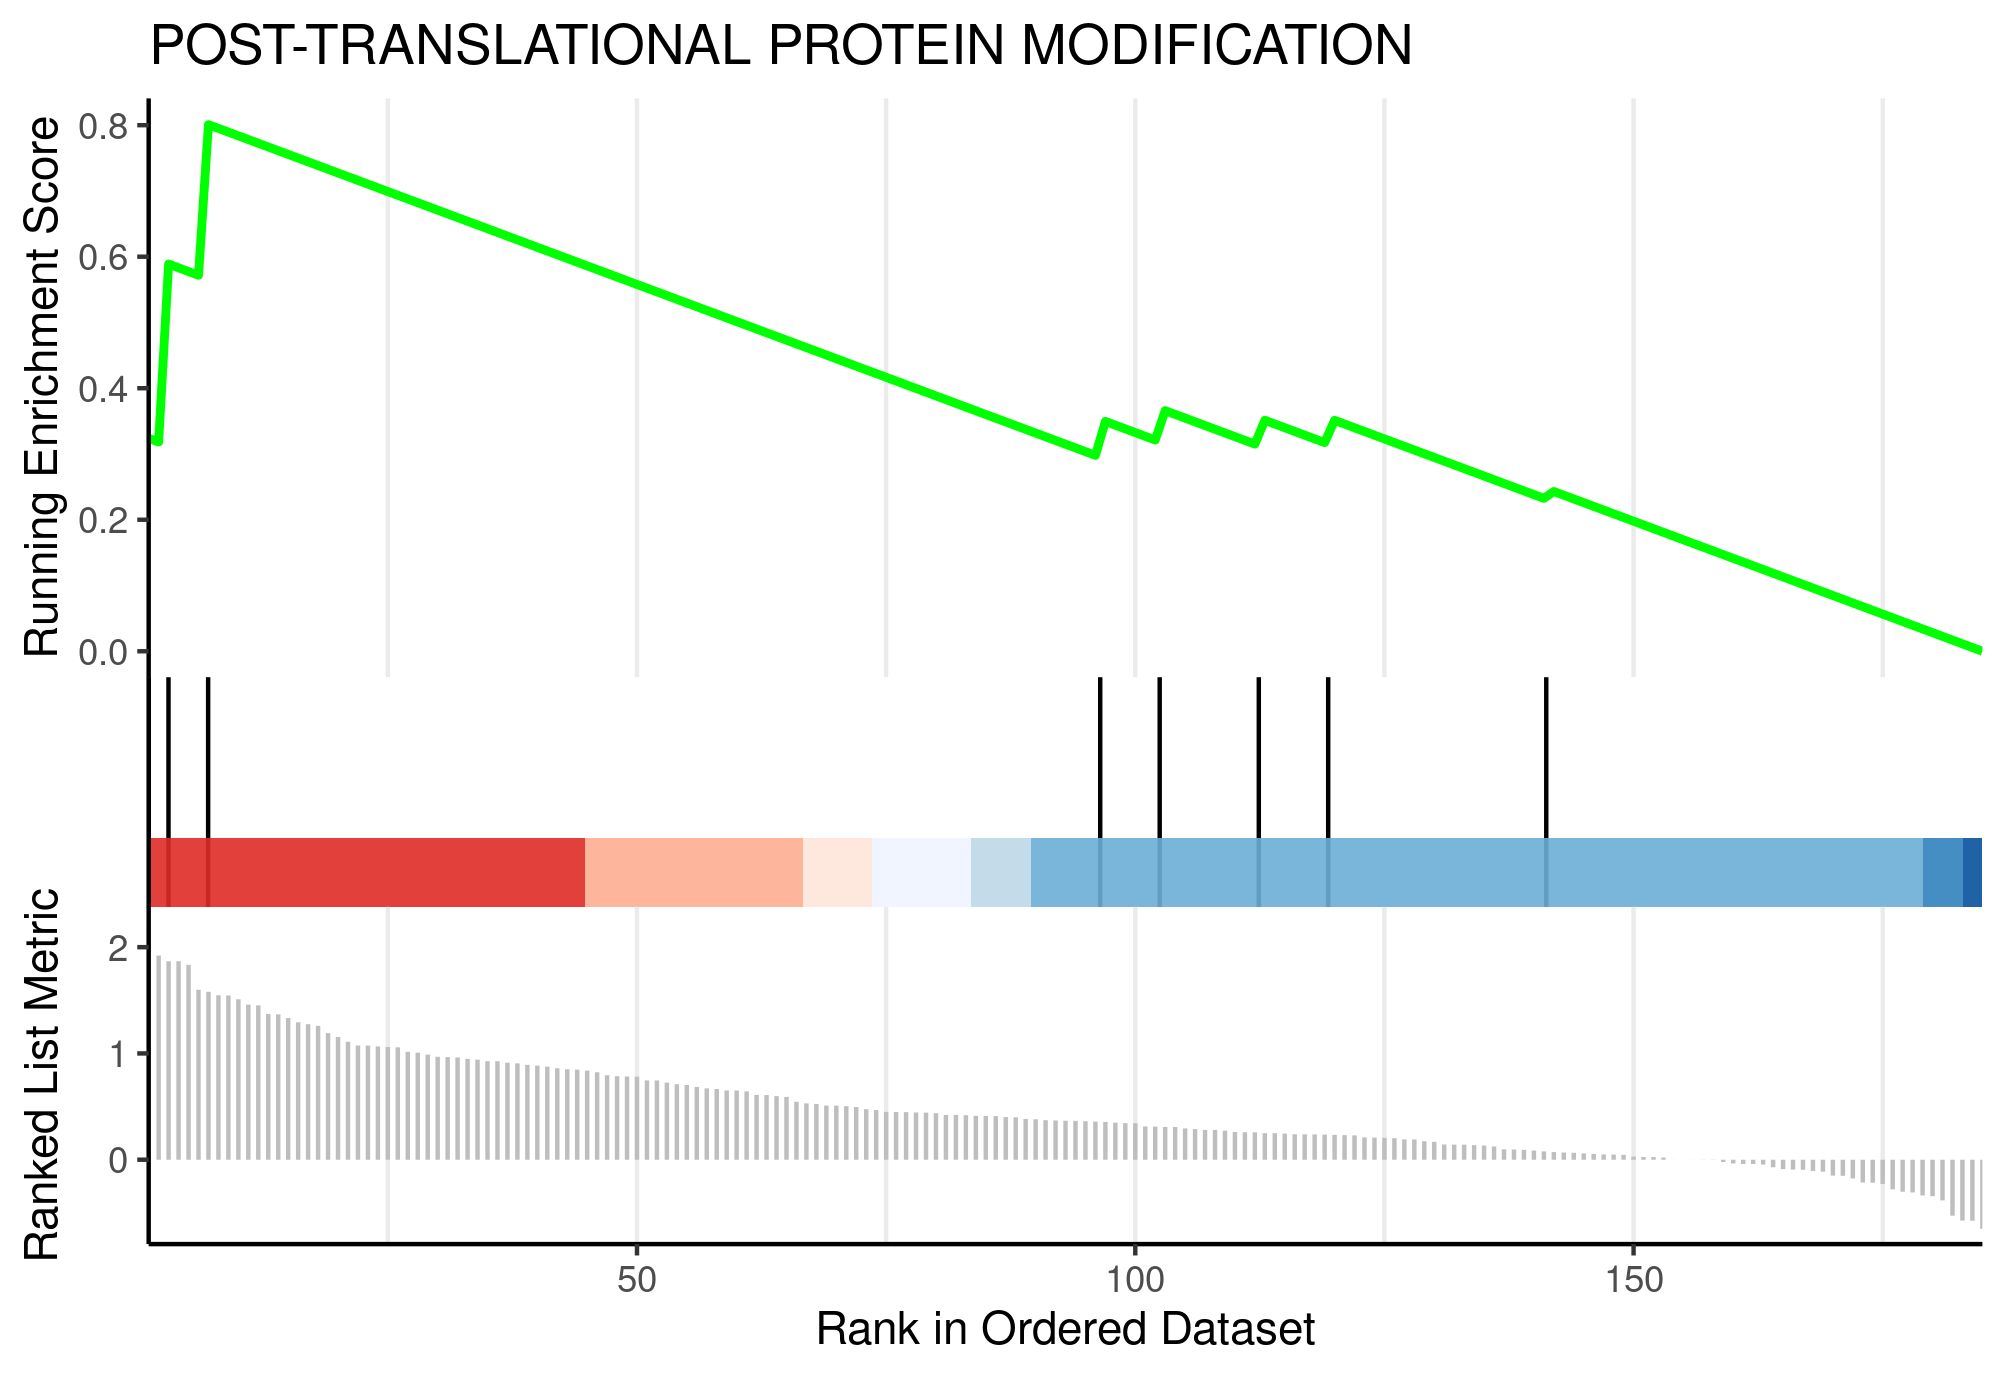
\includegraphics[width=0.49\linewidth]{../Results/Plasma/Comparisons/active_disease_vs_healthy_controls/Univariate/GSEA/GSEA_PLOTS/active_disease_vs_healthy_controls_gseaplot_POST-TRANSLATIO} 

}

\caption{Example of two ES visualizations and calculation. (Left) Downregulation of Notch signaling. (Right) Upregulation of protein modification.}\label{fig:gseaNes}
\end{figure}

\hypertarget{nea}{%
\subsection{NEA}\label{nea}}

NEA or Network Enrichment Analysis is an alternative method to asses which biological functions are regulated following an experiment or when comparing different conditions. As opposed to GSEA, where you look at the overlap of genes in a ranked list and in a gene set directly, in NEA you take the \textbf{number of known associations} between genes found to be significant and a gene set into account. To do this we use the NEA algorithm as implemented in the NEAT R package (see \href{https://bmcbioinformatics.biomedcentral.com/articles/10.1186/s12859-016-1203-6}{paper} for a relatively easy explanation).

Methods paper for NEAT (NEA Test):

The starting point of enrichment analyses is the identification of one or more gene sets of interest. These target gene sets are typically groups of genes that are differentially expressed between experimental conditions, but they can also be different types of gene sets: e.g., clusters of genes that are functionally similar in a given time course, or genes that are bound by a particular protein in a ChIP-chip or ChIP-seq experiment. Enrichment analysis provides a characterization of each target gene set by testing whether some known functional gene sets can be related to it. Methods for gene enrichment analysis assess the relationship between a target gene set and each functional gene set simply by considering the overlap of these two groups. In contrast to this, network enrichment analysis incorporates an evaluation of the level of association between genes in the target set and genes in the functional gene set into the test.

The significant genes were defined here as to have an adjusted p-value smaller than 0.05 and an estimate of either larger than 0 (``upregulated genes'') or smaller thn 0 (``downregulated genes''). The genes set collection consisted of a slimmed down version of the gene set collection used for GSEA (only MSigDB terms for computational resons). The known associations were collected from \href{https://string-db.org}{stringDB}.

Each univariate comparison folder (e.g.~\textbf{Results/Plasma/Comparisons/active\_disease\_vs\_healthy\_controls/Univariate/}) contains a \textbf{NEA/} folder that contains the output of the network enrichment analysis. This output consists of 2 excel files: one containing the results for the upregulated genes (e.g.~active\_disease\_vs\_healthy\_controls\_neat\_up\_results.xlsx) and one containing the results for the downregulated genes (e.g.~active\_disease\_vs\_healthy\_controls\_neat\_down\_results.xlsx).

\hypertarget{multivariate-analysis}{%
\section{Multivariate analysis}\label{multivariate-analysis}}

In addition, a multivariate technique called PLS-DA was used. Information about this method can be found \href{https://bmcbioinformatics.biomedcentral.com/articles/10.1186/1471-2105-12-253}{here} and \href{http://mixomics.org/case-studies/splsda-srbct/}{here}. This method attempts to represent the data in a lower dimensional set of ``components'', similarly to PCA. Unlike PCA, which attempts to retain as much variation of one dataset in the components, PLS methods try to maximize the covariance between two datasets (here the expression data and the phenotype data). In this way, the phenotype separation will be maximized. PLS-DA attempts to find the most optimal way to represent multidimensional data taking sample classes into account using as little components as possible.

To better understand how this ``black box'' model works, the samples are visualized in the reduced PLS space (see Figure \ref{fig:plsPlot} (Left)). In this plot healthy controls separate quite well from the active disease samples on - mainly - Component 1. By looking at which proteins contribute the strongest to Component 1 (see Figure \ref{fig:plsPlot} (Right)), one can get an idea of which proteins are most important in separating these two phenotypes. The proteins with the highest absolute loadings will drive the separation the most. For example, a protein with a high positive loading on component 1 will contribute significantly to the separation on component 1. Moreover, a \textbf{positive} loading value on component 1 indicates that the expression of that protein is also higher in samples that have a higher component 1 value. a \textbf{negative} loading value on component 1 indicates that the expression of that protein is lower in samples that have a higher component 1 value. Looking at and combining these plots, one can get an idea on how the samples are separated and which proteins are important to drive this separation.

\begin{figure}

{\centering 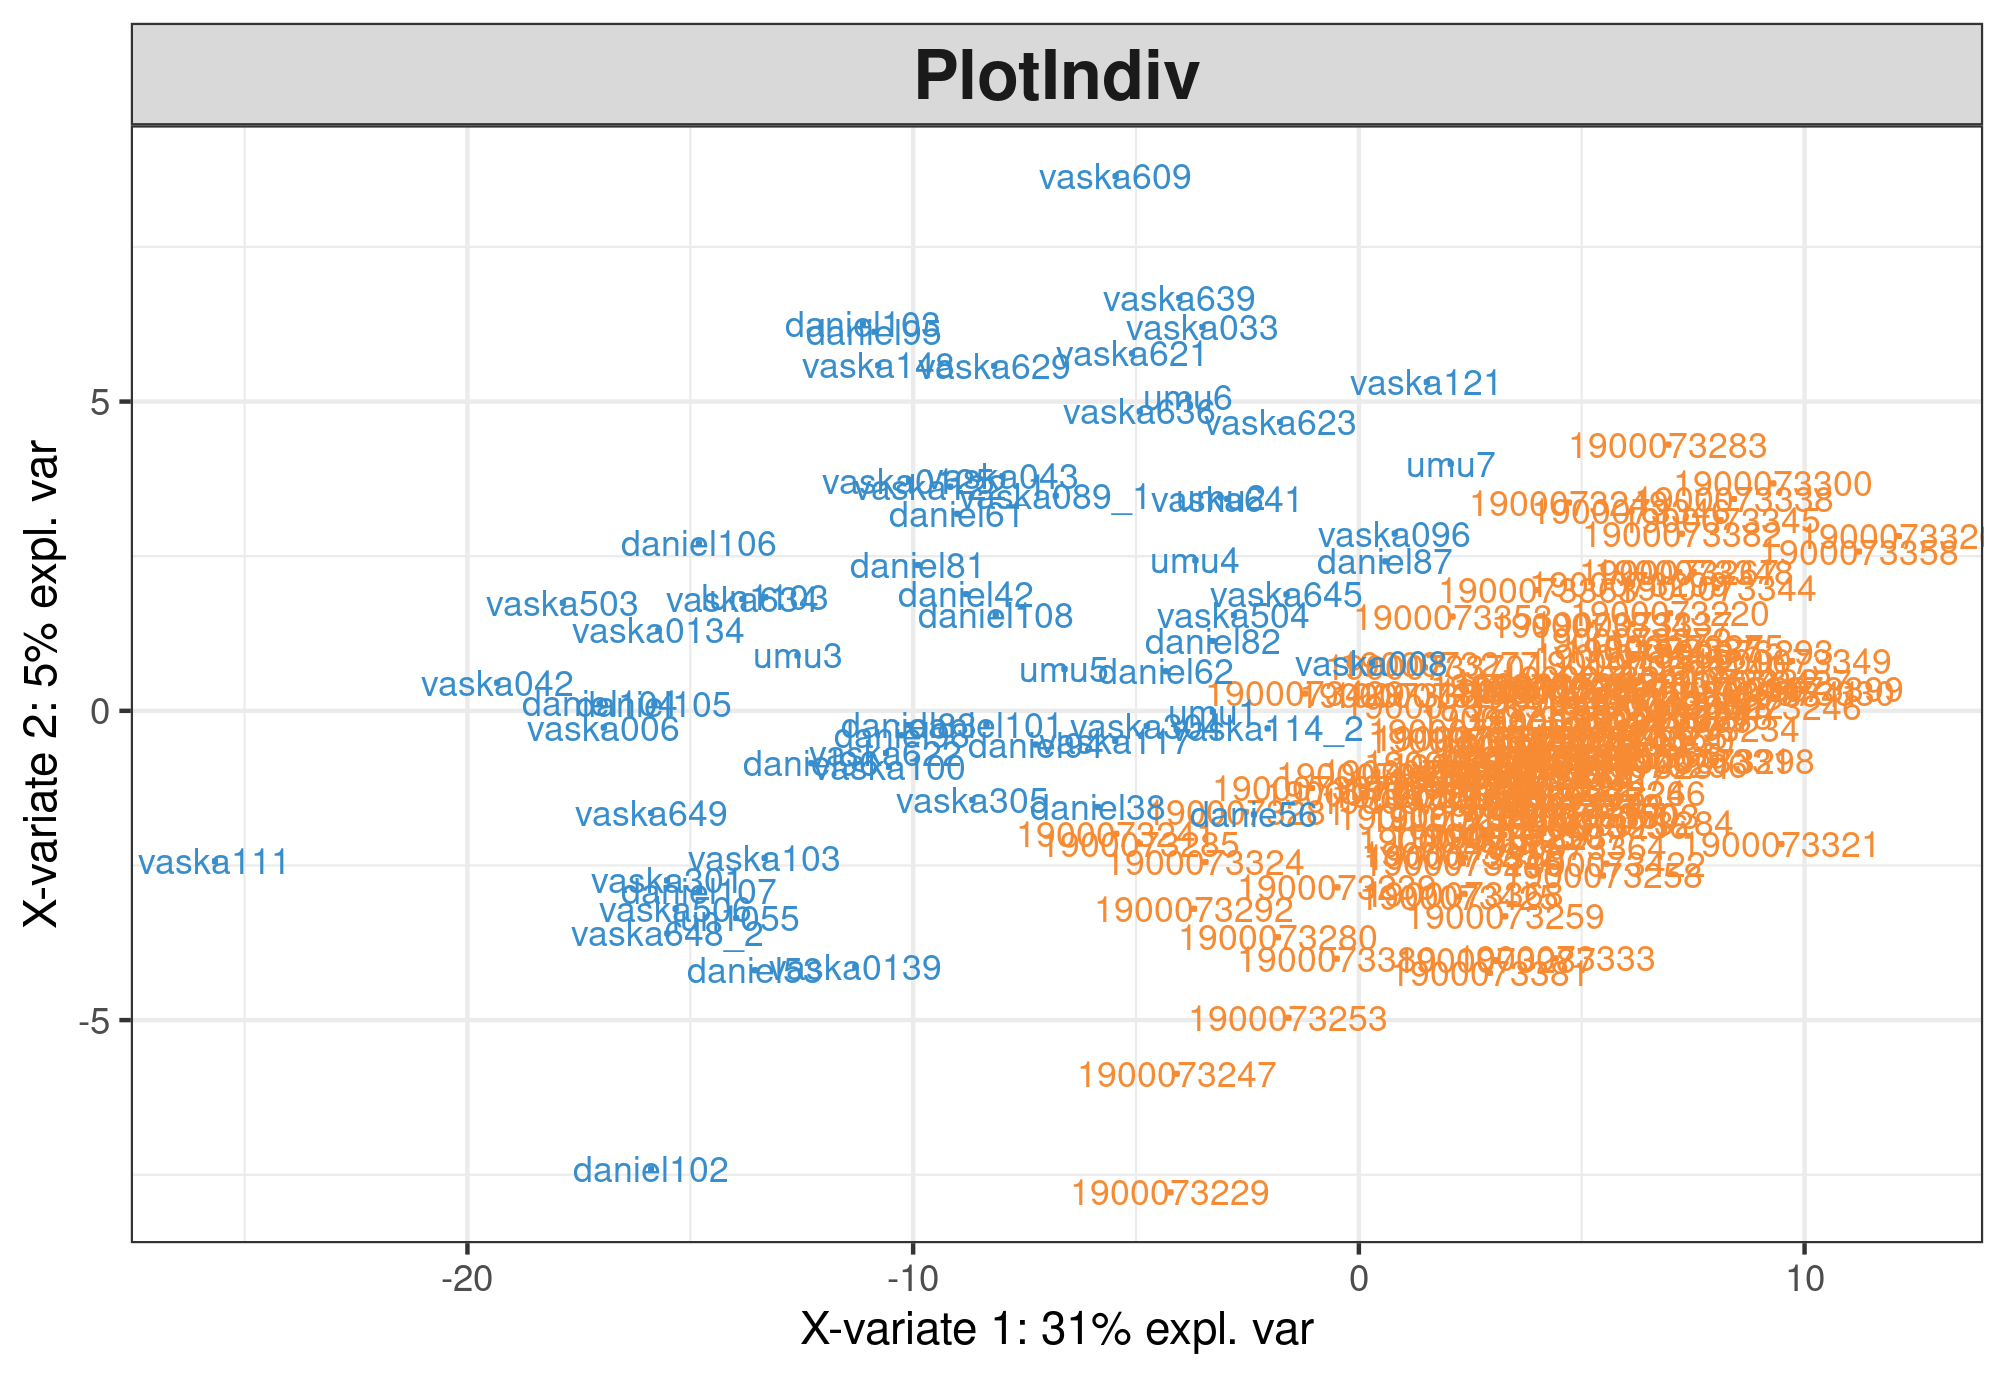
\includegraphics[width=0.49\linewidth]{../Results/Plasma/Comparisons/active_disease_vs_healthy_controls/Multivariate/active_disease_vs_healthy_controls_SamplePlot_2comp} 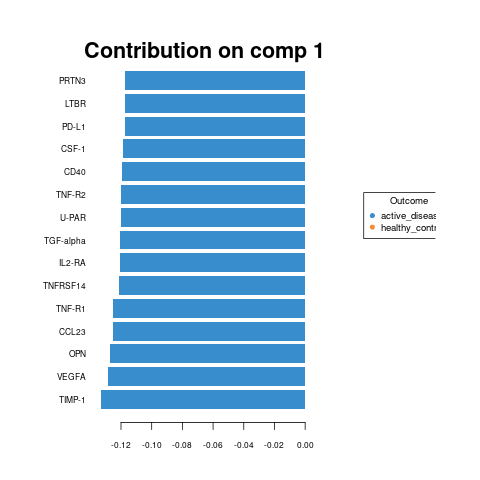
\includegraphics[width=0.49\linewidth]{../Results/Plasma/Comparisons/active_disease_vs_healthy_controls/Multivariate/active_disease_vs_healthy_controls_Loadings_Comp1_Top15} 

}

\caption{PLS-DA visualization. (Left) Samples projected into the subspace spanned by the first two PLS components. (Right) top 15 of loading weights on Component 1, color indicates the class for which the selected variable has a maximal mean value.}\label{fig:plsPlot}
\end{figure}

Results for the PLS-DA analysis are collected in \textbf{Results/Plasma/Comparisons/\{comparison\}\}/Multivariate/} and \textbf{Results/Serum/Comparisons/\{comparison\}\}/Multivariate/}.

The loading weights for all proteins on the first 5 components can be found in in an excel file (e.g.~active\_disease\_vs\_healthy\_controls\_Loadings\_Scores.xlsx). In the same folder, visualization of the samples in the PLS subspace spanned by the first 2 components, the top 15 loading weights on Comp 1 and 2 and a biplot showing the samples nd most significant proteins on the same plot are collected.

\hypertarget{correlation}{%
\chapter{Correlation}\label{correlation}}

Pearson correlations of each protein versus crp, sr and bvas values were calculated.

\hypertarget{crp}{%
\section{crp}\label{crp}}

The full list of protein-wise pearson correlation results with crp is collected in excel files in \textbf{Results/Plasma/Correlation/crp/crp\_pearson\_correlation.xlsx} and \textbf{Results/Serum/Correlation/crp/crp\_pearson\_correlation.xlsx}

All individuals regressions are plotted and collected in the subfolder \textbf{regression\_plots/} (see Figure \ref{fig:crpCorr})

\textbackslash begin\{figure\}

\{\centering 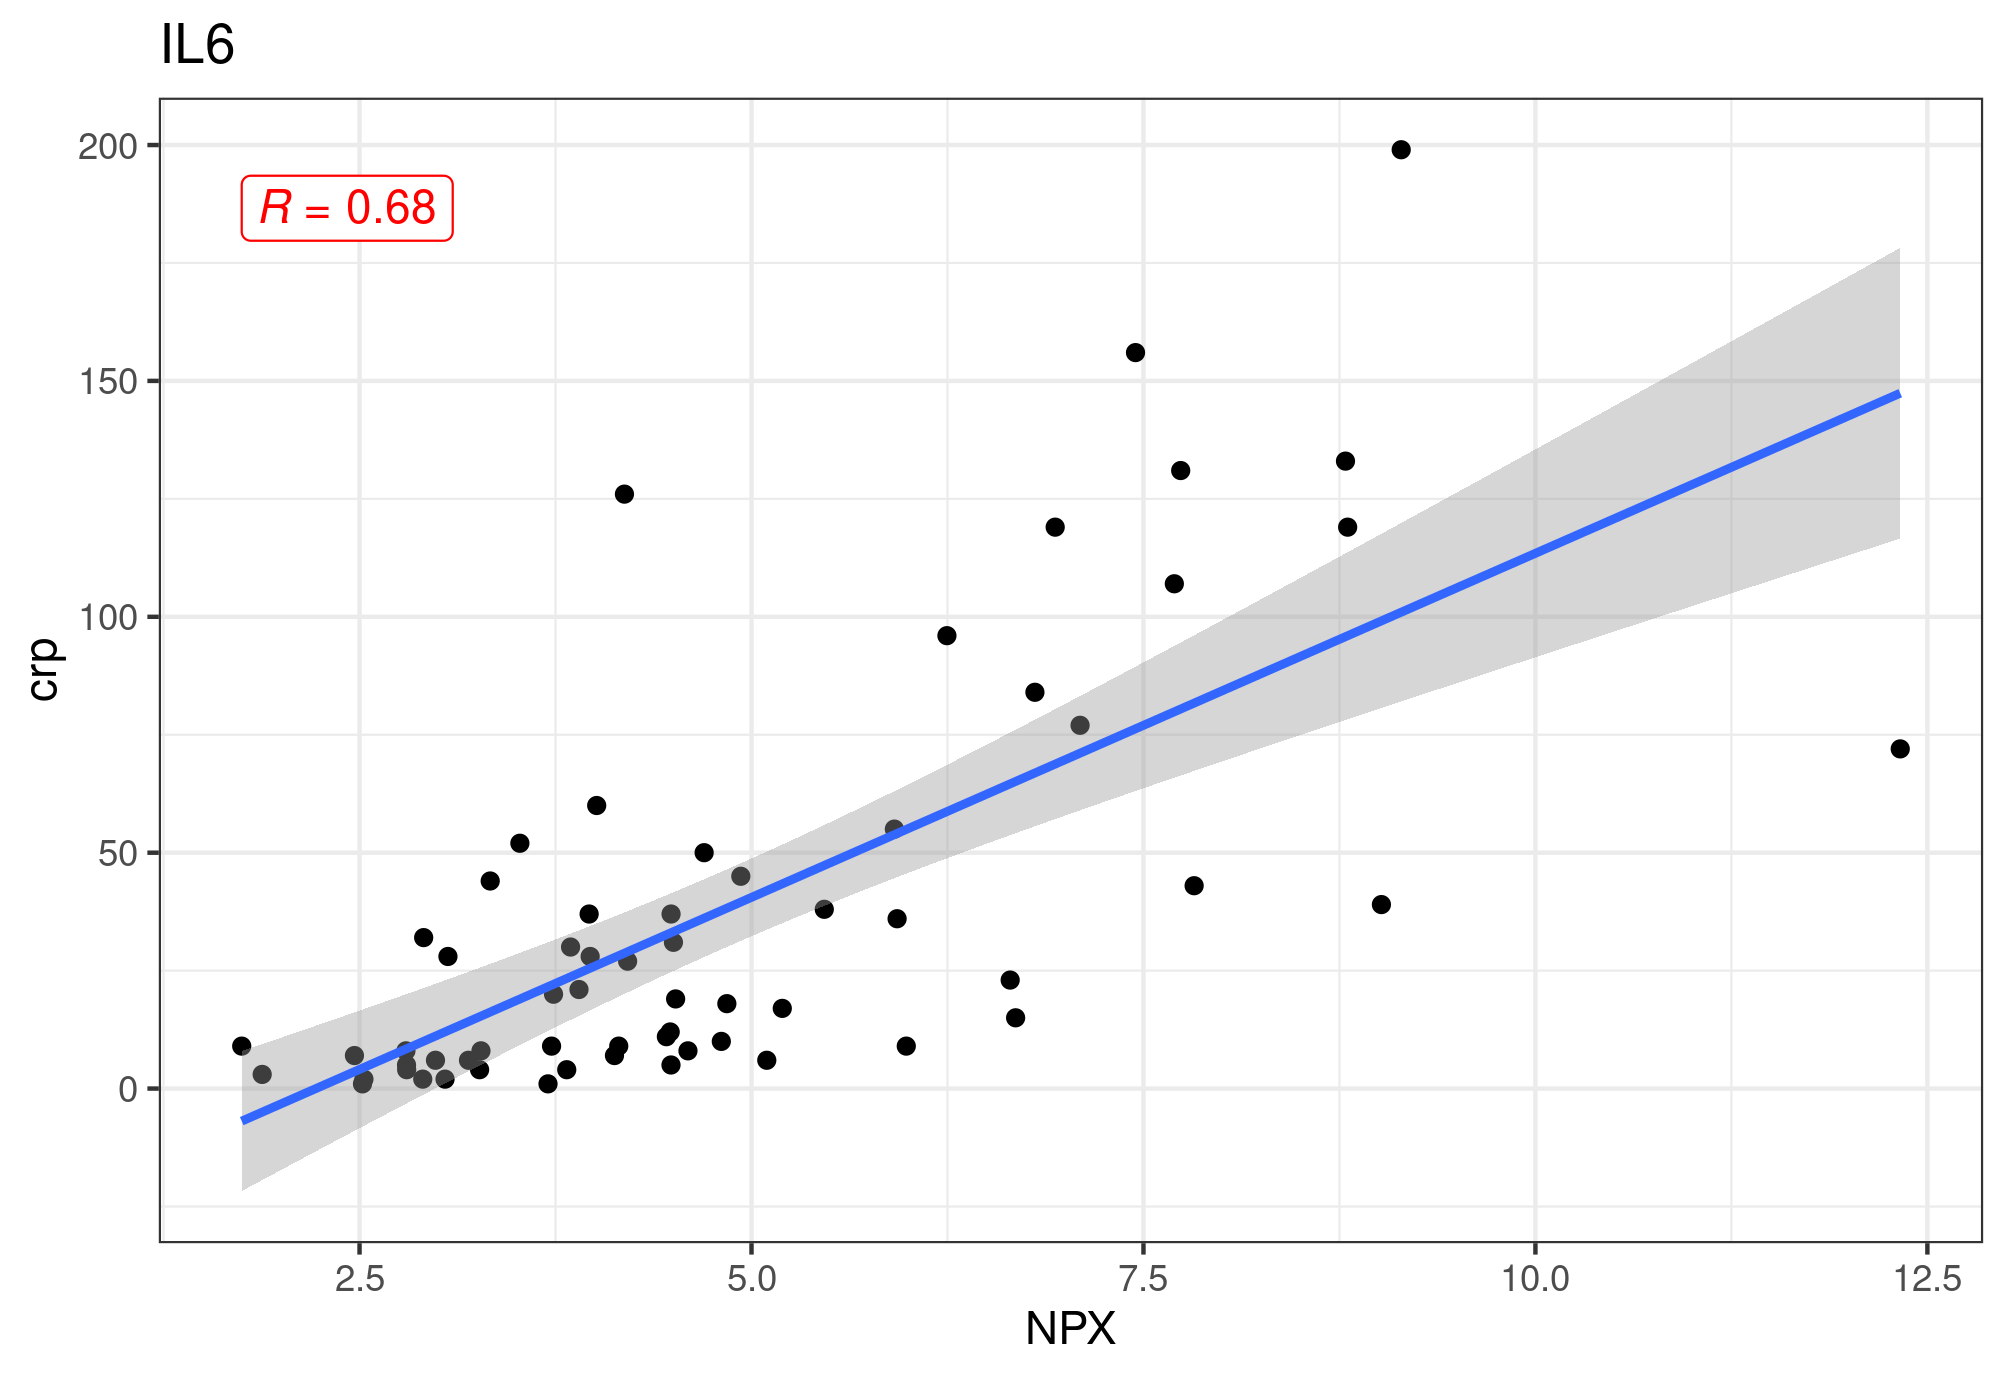
\includegraphics[width=0.49\linewidth]{../Results/Plasma/Correlation/crp/regression_plots/IL6_regression} \includegraphics[width=0.49\linewidth]{../Results/Plasma/Correlation/crp/regression_plots/SCF_regression}

\}

\textbackslash caption\{Most significant positively crp correlated protein (Left) Most significant negatively crp correlated protein (Right). Indicated in red is the pearson correlation coefficient and 95\% confidence interval in grey\}\label{fig:crpCorr}
\textbackslash end\{figure\}

\hypertarget{sr}{%
\section{sr}\label{sr}}

The full list of protein-wise pearson correlation results with sr is collected in excel files in \textbf{Results/Plasma/Correlation/sr/sr\_pearson\_correlation.xlsx} and \textbf{Results/Serum/Correlation/sr/sr\_pearson\_correlation.xlsx}

All individuals regressions are plotted and collected in the subfolder \textbf{regression\_plots/} (see Figure \ref{fig:srCorr})

\textbackslash begin\{figure\}

\{\centering 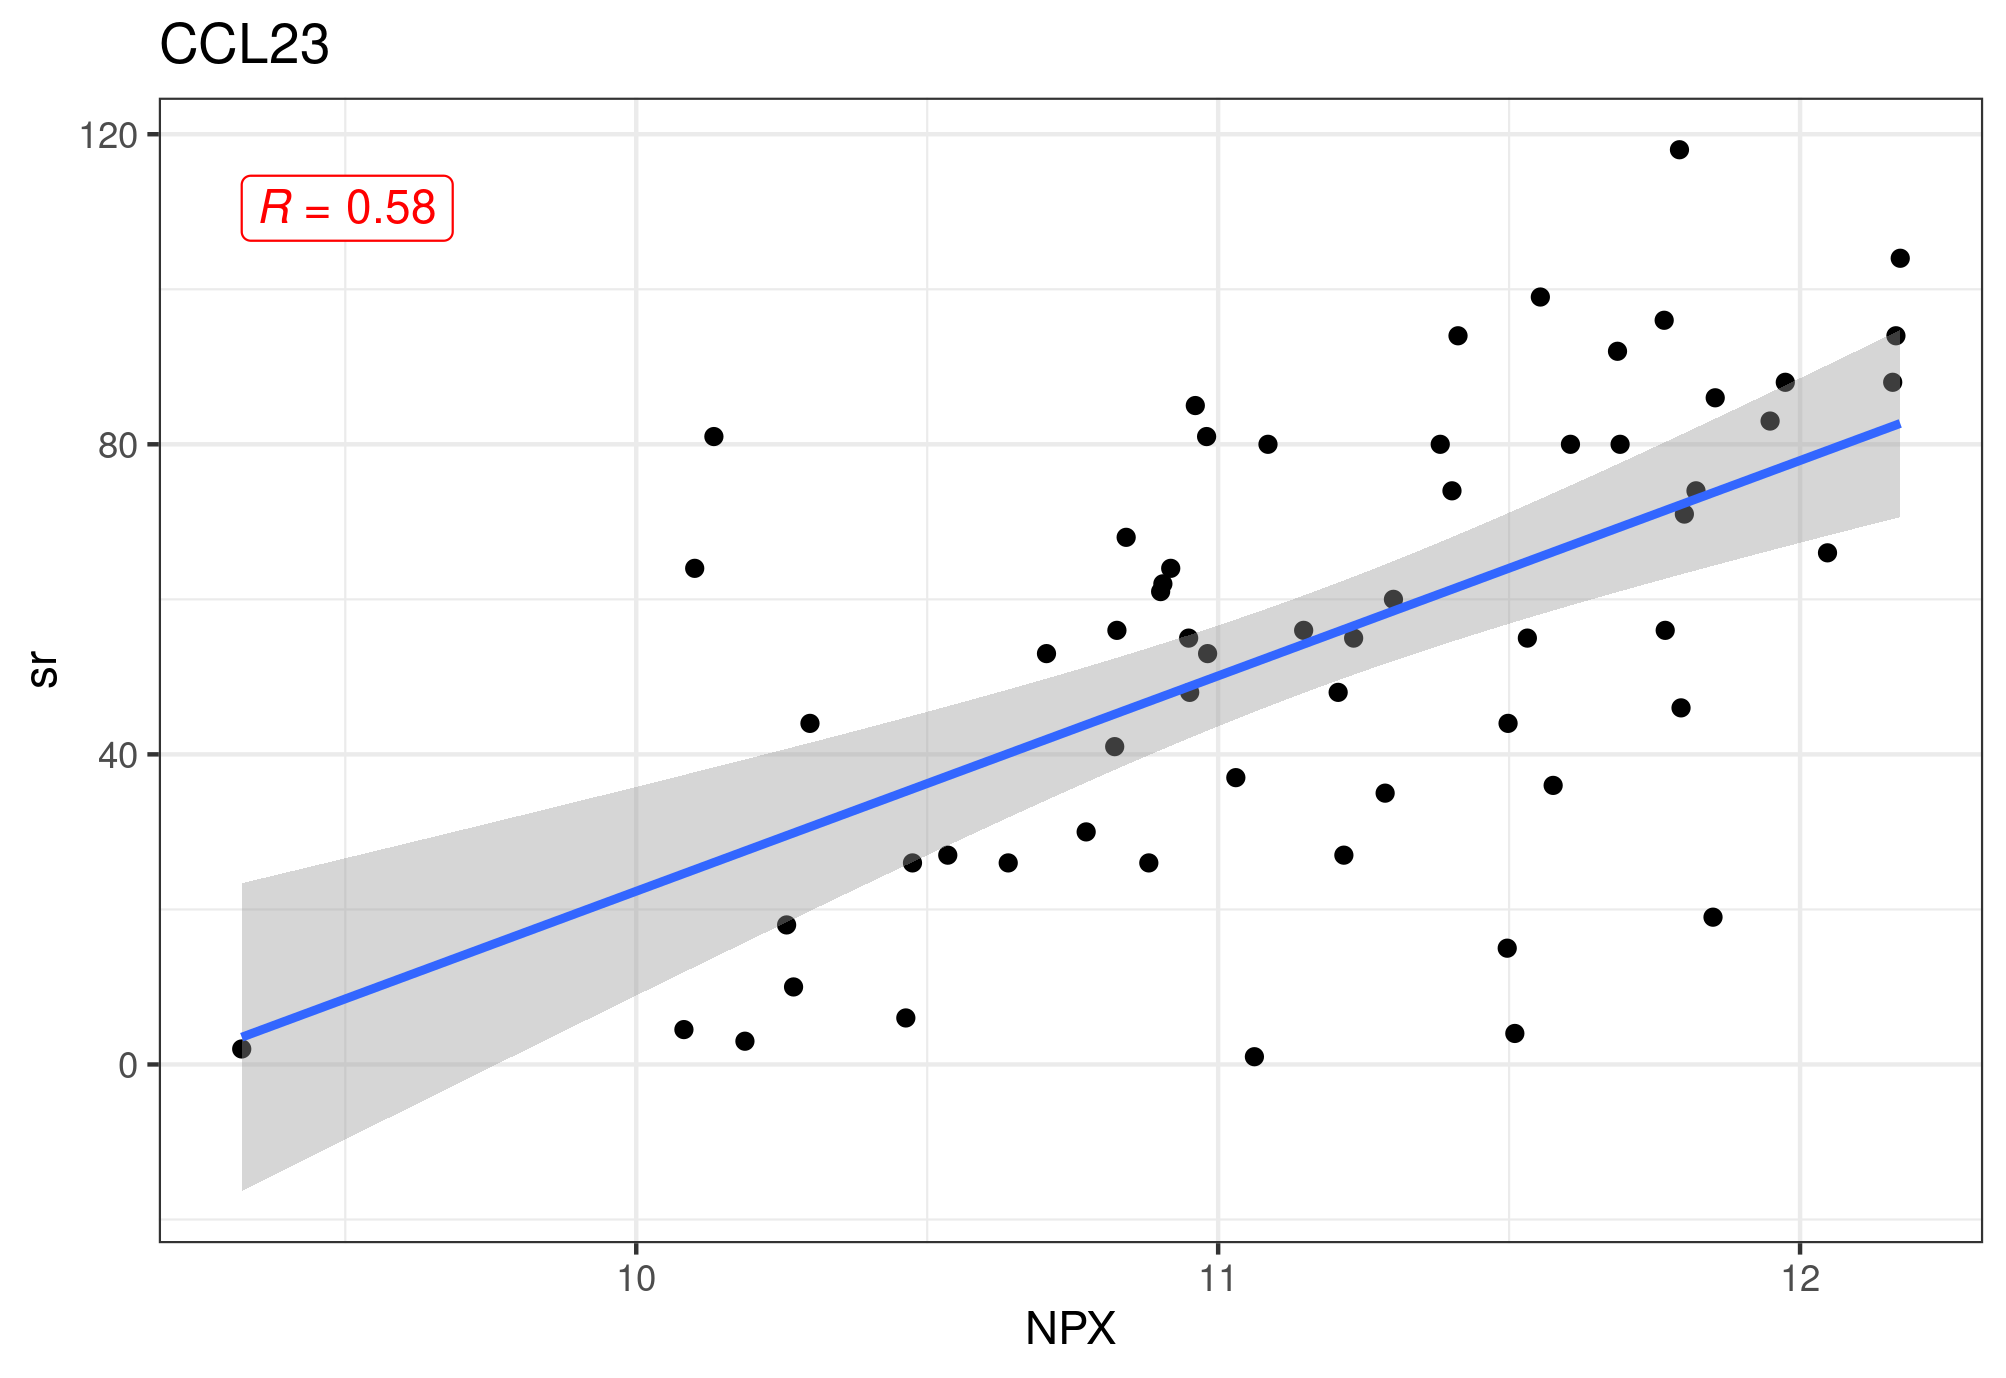
\includegraphics[width=0.49\linewidth]{../Results/Plasma/Correlation/sr/regression_plots/CCL23_regression} \includegraphics[width=0.49\linewidth]{../Results/Plasma/Correlation/sr/regression_plots/SCF_regression}

\}

\textbackslash caption\{Most significant positively sr correlated protein (Left) Most significant negatively sr correlated protein (Right). Indicated in red is the pearson correlation coefficient and 95\% confidence interval in grey\}\label{fig:srCorr}
\textbackslash end\{figure\}

\hypertarget{bvas}{%
\section{bvas}\label{bvas}}

The full list of protein-wise pearson correlation results with bvas is collected in excel files in \textbf{Results/Plasma/Correlation/bvas/bvas\_pearson\_correlation.xlsx} and \textbf{Results/Serum/Correlation/bvas/bvas\_pearson\_correlation.xlsx}

All individuals regressions are plotted and collected in the subfolder \textbf{regression\_plots/} (see Figure \ref{fig:bvasCorr})

\textbackslash begin\{figure\}

\{\centering 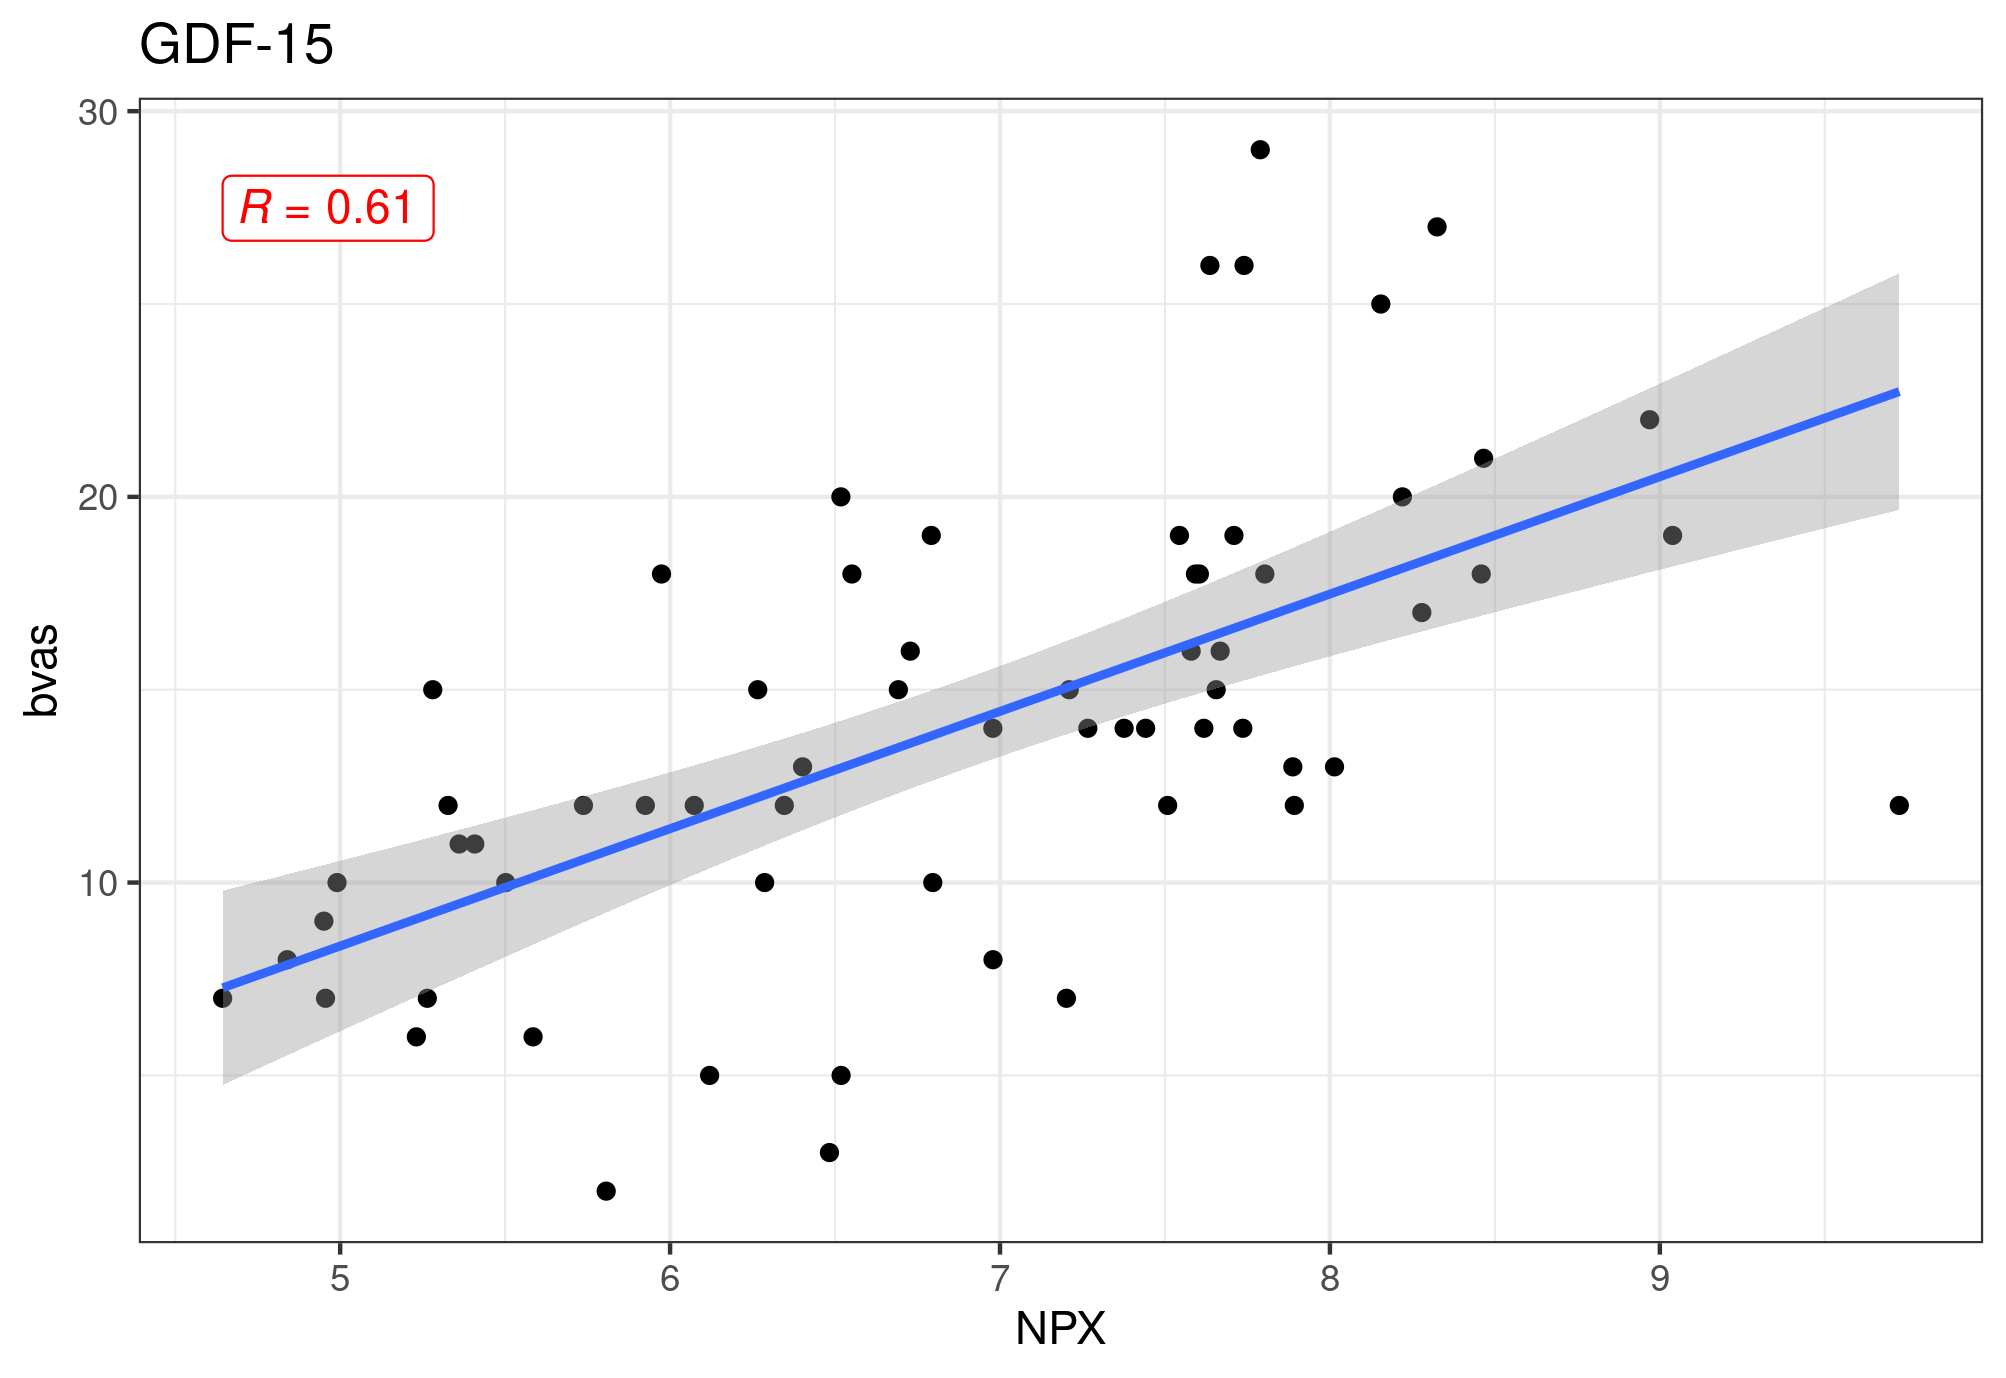
\includegraphics[width=0.49\linewidth]{../Results/Plasma/Correlation/bvas/regression_plots/GDF-15_bvas_correlation} 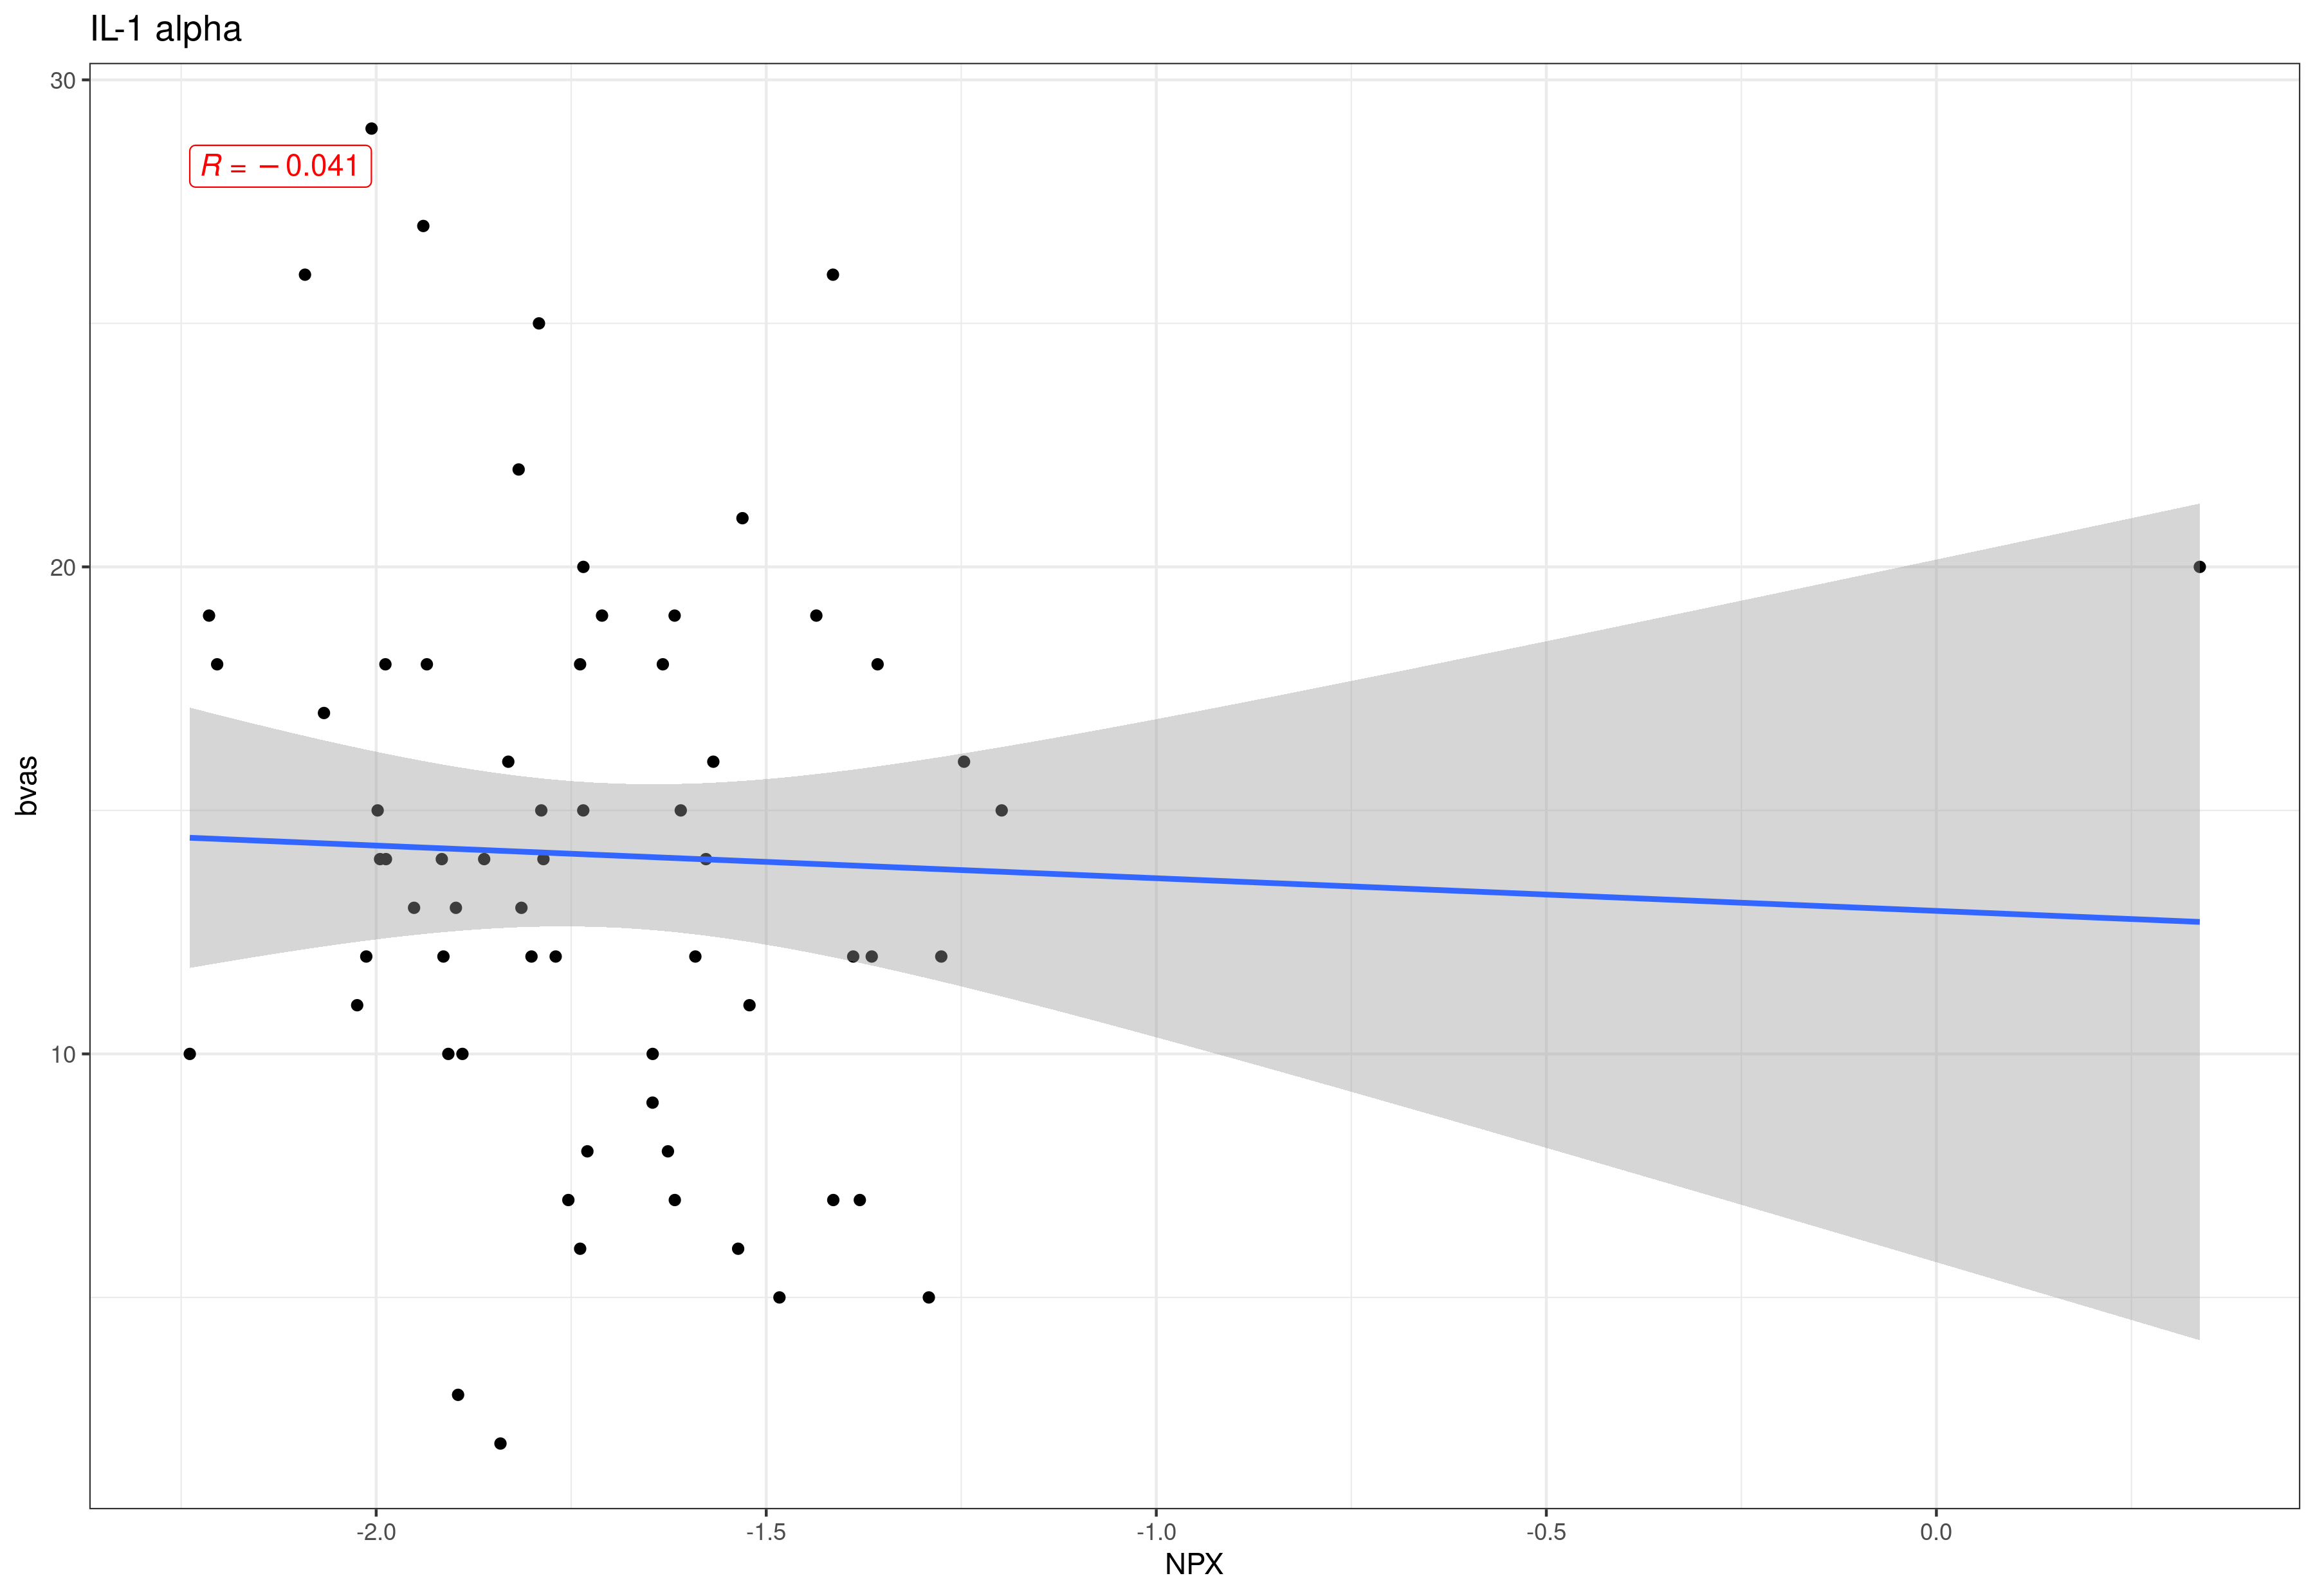
\includegraphics[width=0.49\linewidth]{../Results/Plasma/Correlation/bvas/regression_plots/IL-1 alpha_bvas_correlation}

\}

\textbackslash caption\{Most significant positively bvas correlated protein (Left) Most significant negatively bvas correlated protein (Right). Indicated in red is the pearson correlation coefficient and 95\% confidence interval in grey\}\label{fig:bvasCorr}
\textbackslash end\{figure\}

\hypertarget{cortisone}{%
\chapter{Cortisone}\label{cortisone}}

\hypertarget{protein-level-1}{%
\section{Protein-level}\label{protein-level-1}}

Active disease samples were split in an experimental group that was treated with cortisone and a control group that was not treated with cortisone. Differential analysis between both groups was calculated as in Section 4.1; i.e.~per-protein anova on \emph{age} and \emph{ckd\_epi} corrected data followed by a post-hoc analysis.

Results for the per-protein analysis is collected in \textbf{Results/Plasma/Cortisone} and \textbf{Results/Serum/Cortisone}.

The volcano plot for cortisone vs no\_cortisone is shown in Figure \ref{fig:cortplots} (Left).

\begin{figure}

{\centering 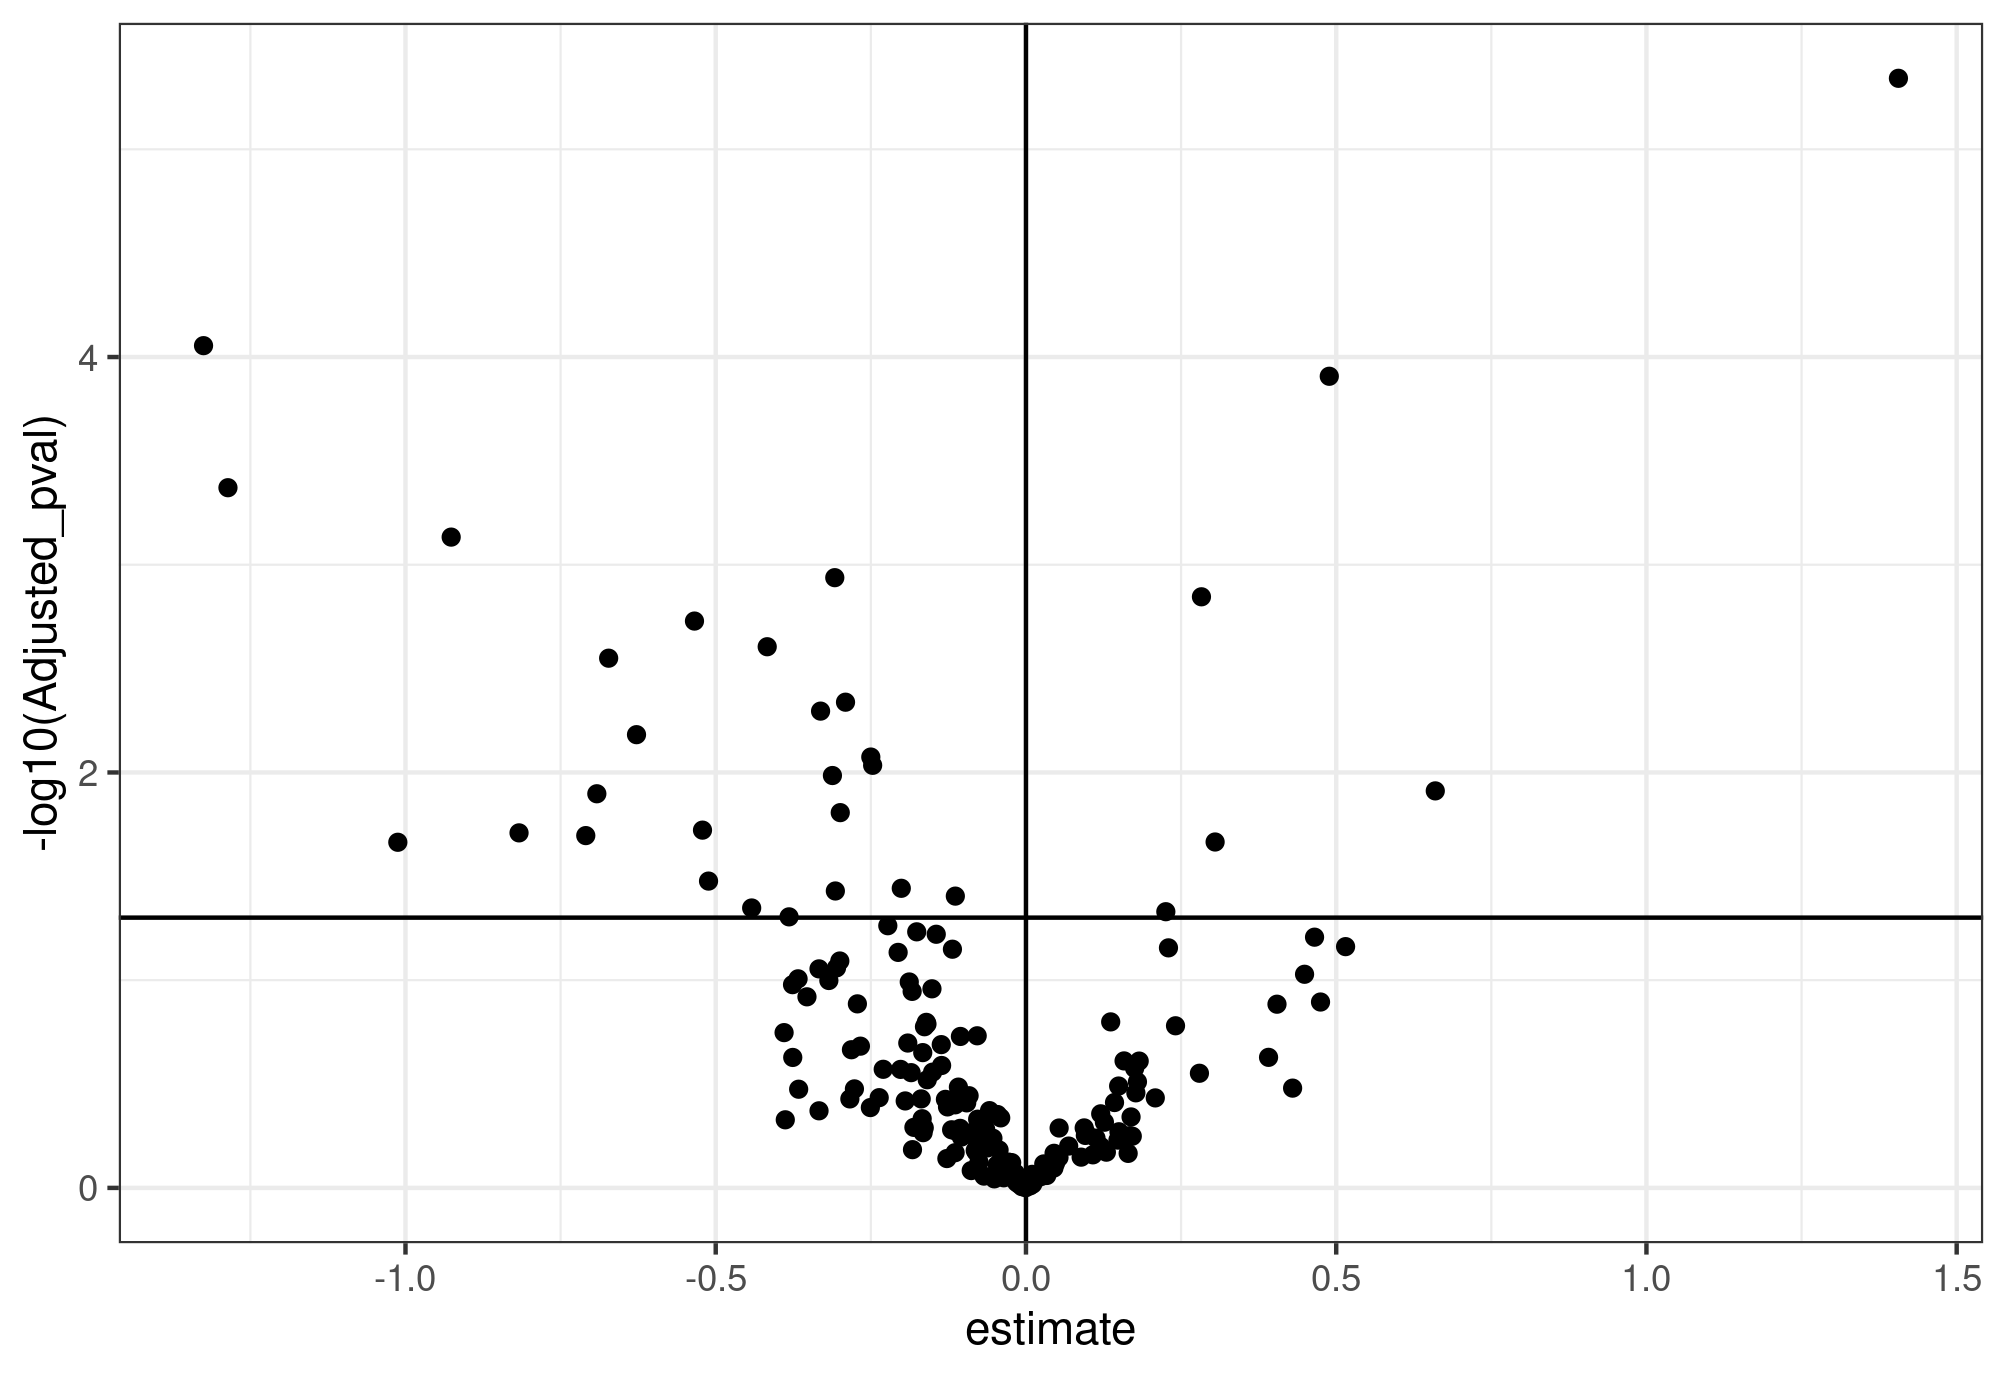
\includegraphics[width=1\linewidth]{../Results/Plasma/Cortisone/Cortisone_vs_No_Cortisone/Univariate/Cortisone_vs_No_Cortisone_volcano_anova_posthoc} 

}

\caption{Volcano plot of cortisone versus no cortisone. Horizontal line indicates an adjusted p-value of 0.05}\label{fig:cortplots}
\end{figure}

The top 15 of most significantly regulated proteins (ranked by adjusted p-value) of cortisone versus no\_cortisone is shown in \ref{fig:top15Cort}. The ``estimate'' column can be considered as a log2 fold change (i.e.~a difference of 1 indicates a doubled expression).

\begin{figure}

{\centering 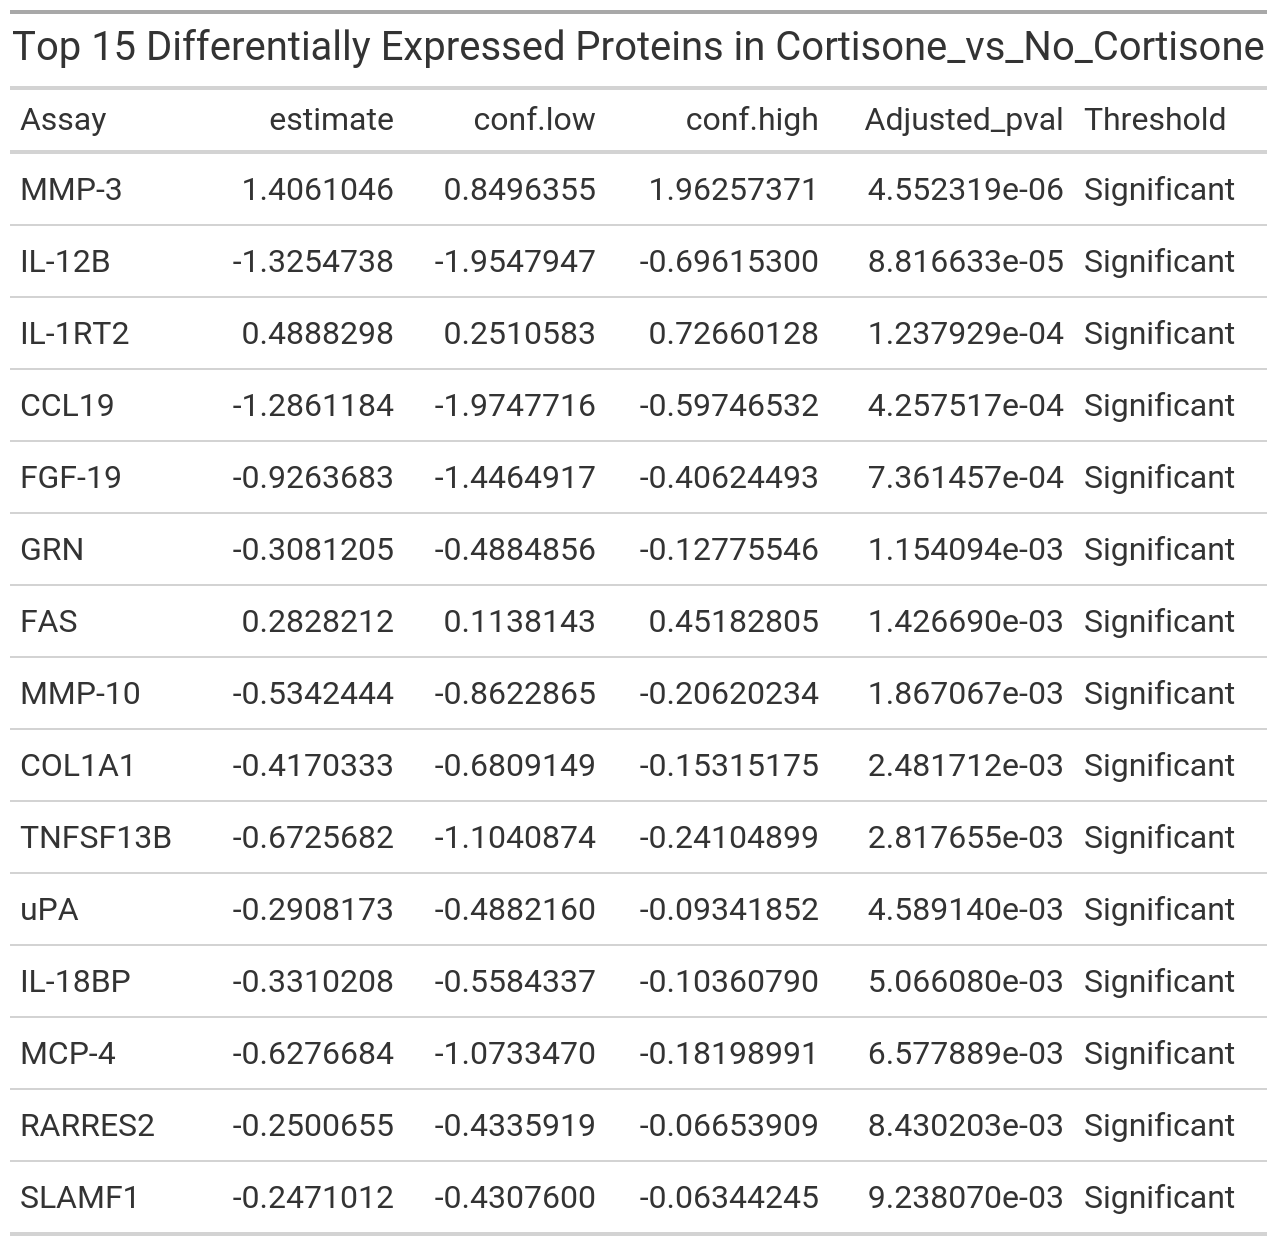
\includegraphics[width=0.75\linewidth]{../Results/Plasma/Cortisone/Cortisone_vs_No_Cortisone/Univariate/Cortisone_vs_No_Cortisone_Top15_table} 

}

\caption{Table of 15 most DE proteins}\label{fig:top15Cort}
\end{figure}

\hypertarget{gsea-1}{%
\section{GSEA}\label{gsea-1}}

GSEA was performed for cortisone versus no\_cortisone as in Section 4.1.2.

As before, the GSEA results folder in the Cortisone folder contains a .xlsx file containing the full GSEA results and two different visualizations of the top terms (see Figure \ref{fig:gseaPlotsCort}). These figures include a barplot of the gene sets with the 6 highest and 6 lowest NES values and an Enrichment map of the 20 gene sets with the highest absolute NES values. Enrichment maps organize gene sets into a network with edges connecting overlapping gene sets. In this way, mutually overlapping gene sets tend to cluster together, making it easier to identify functional modules.

\begin{figure}

{\centering 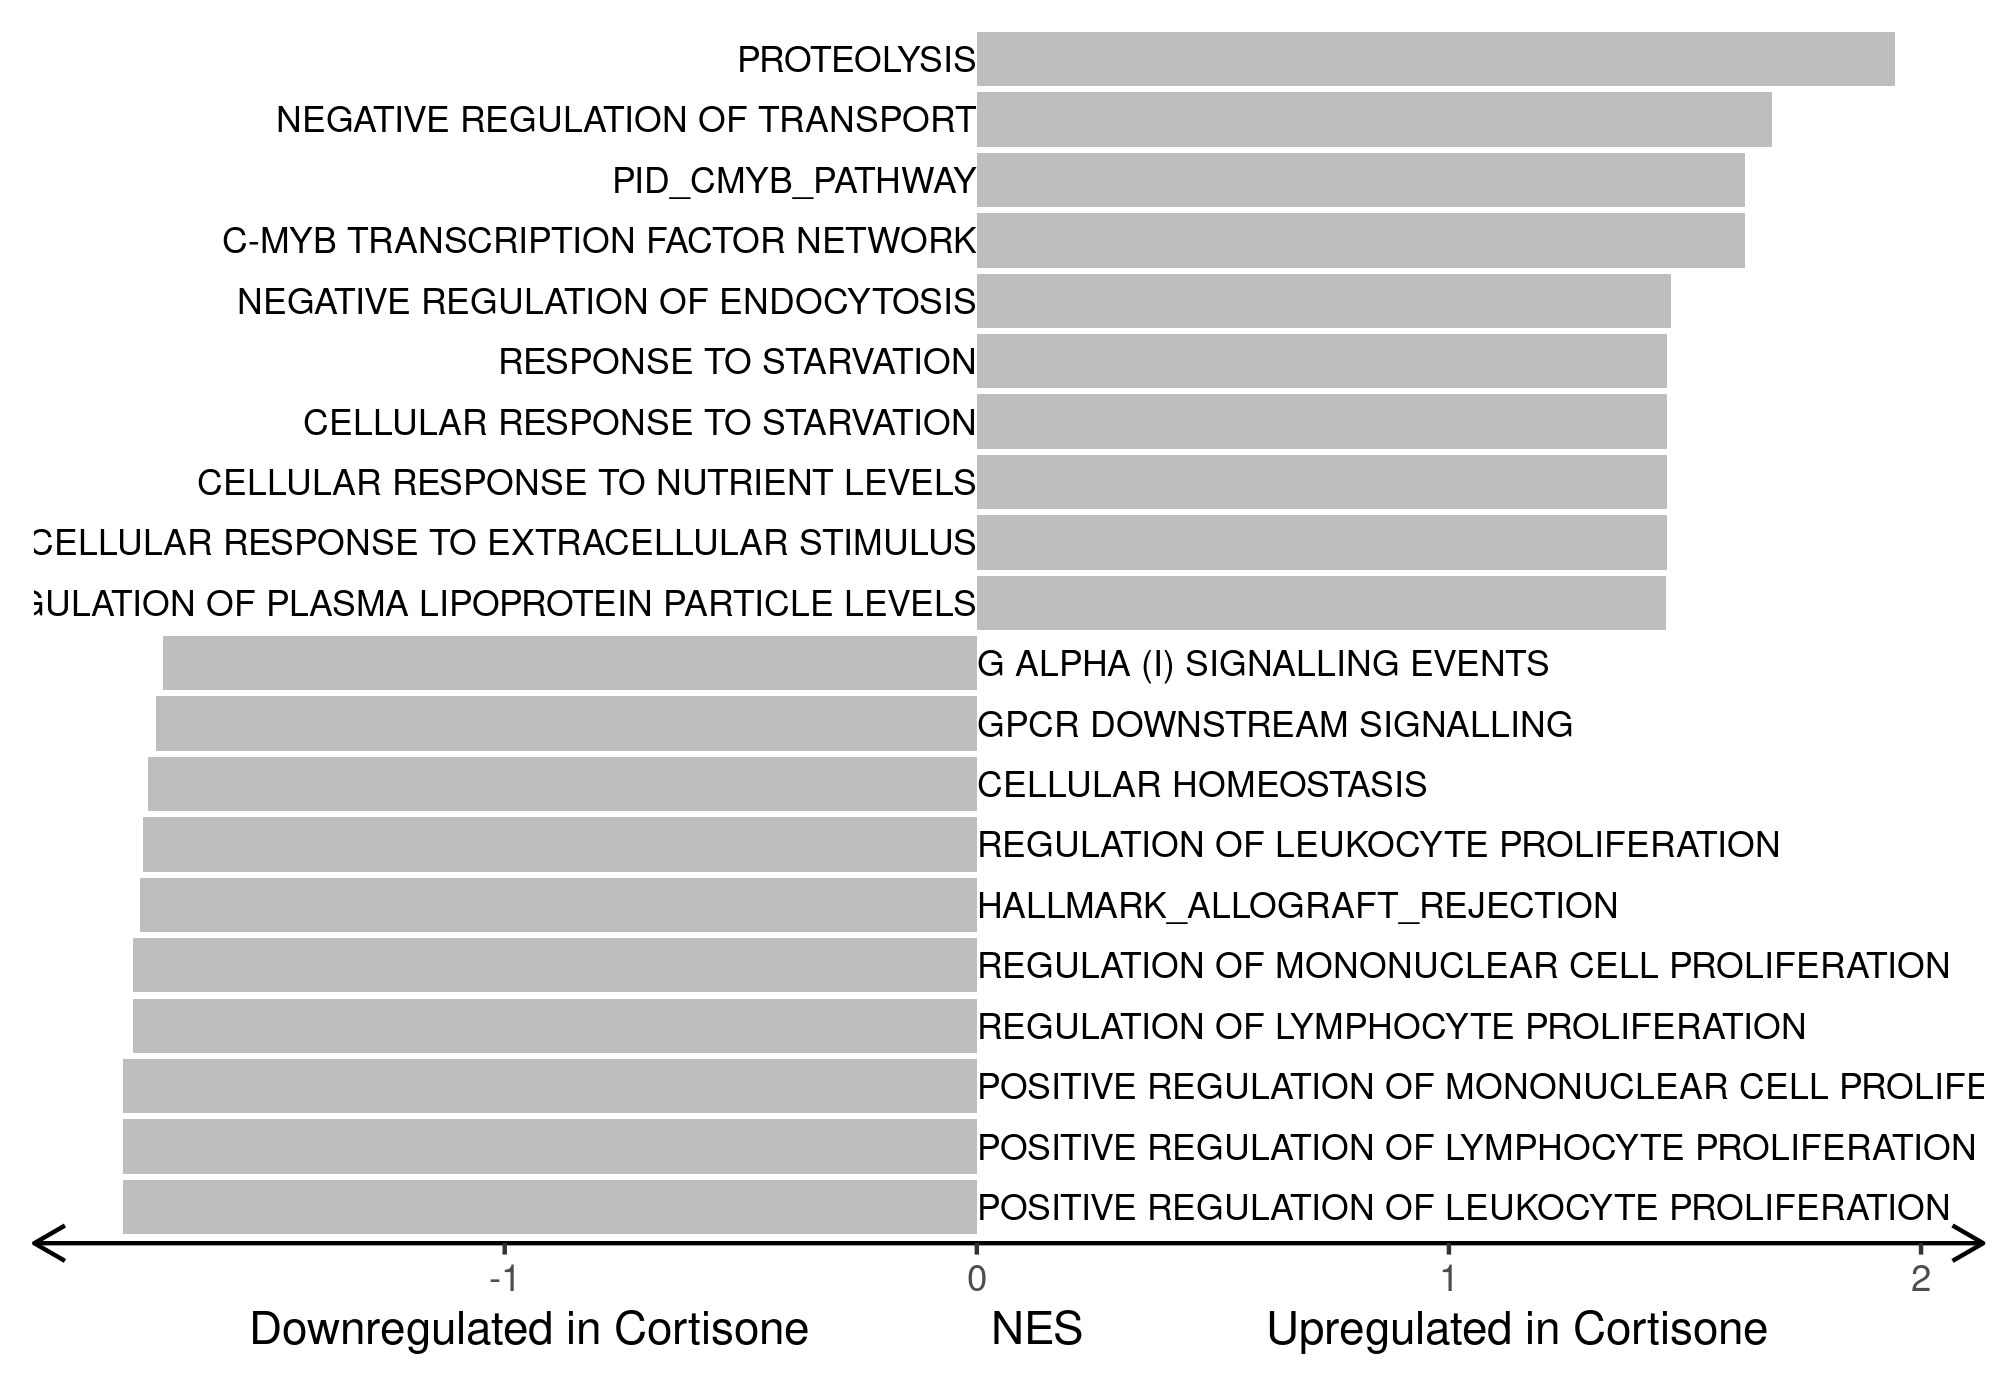
\includegraphics[width=0.49\linewidth]{../Results/Plasma/Cortisone/Cortisone_vs_No_Cortisone/Univariate/GSEA/Cortisone_vs_No_Cortisone_barplot} 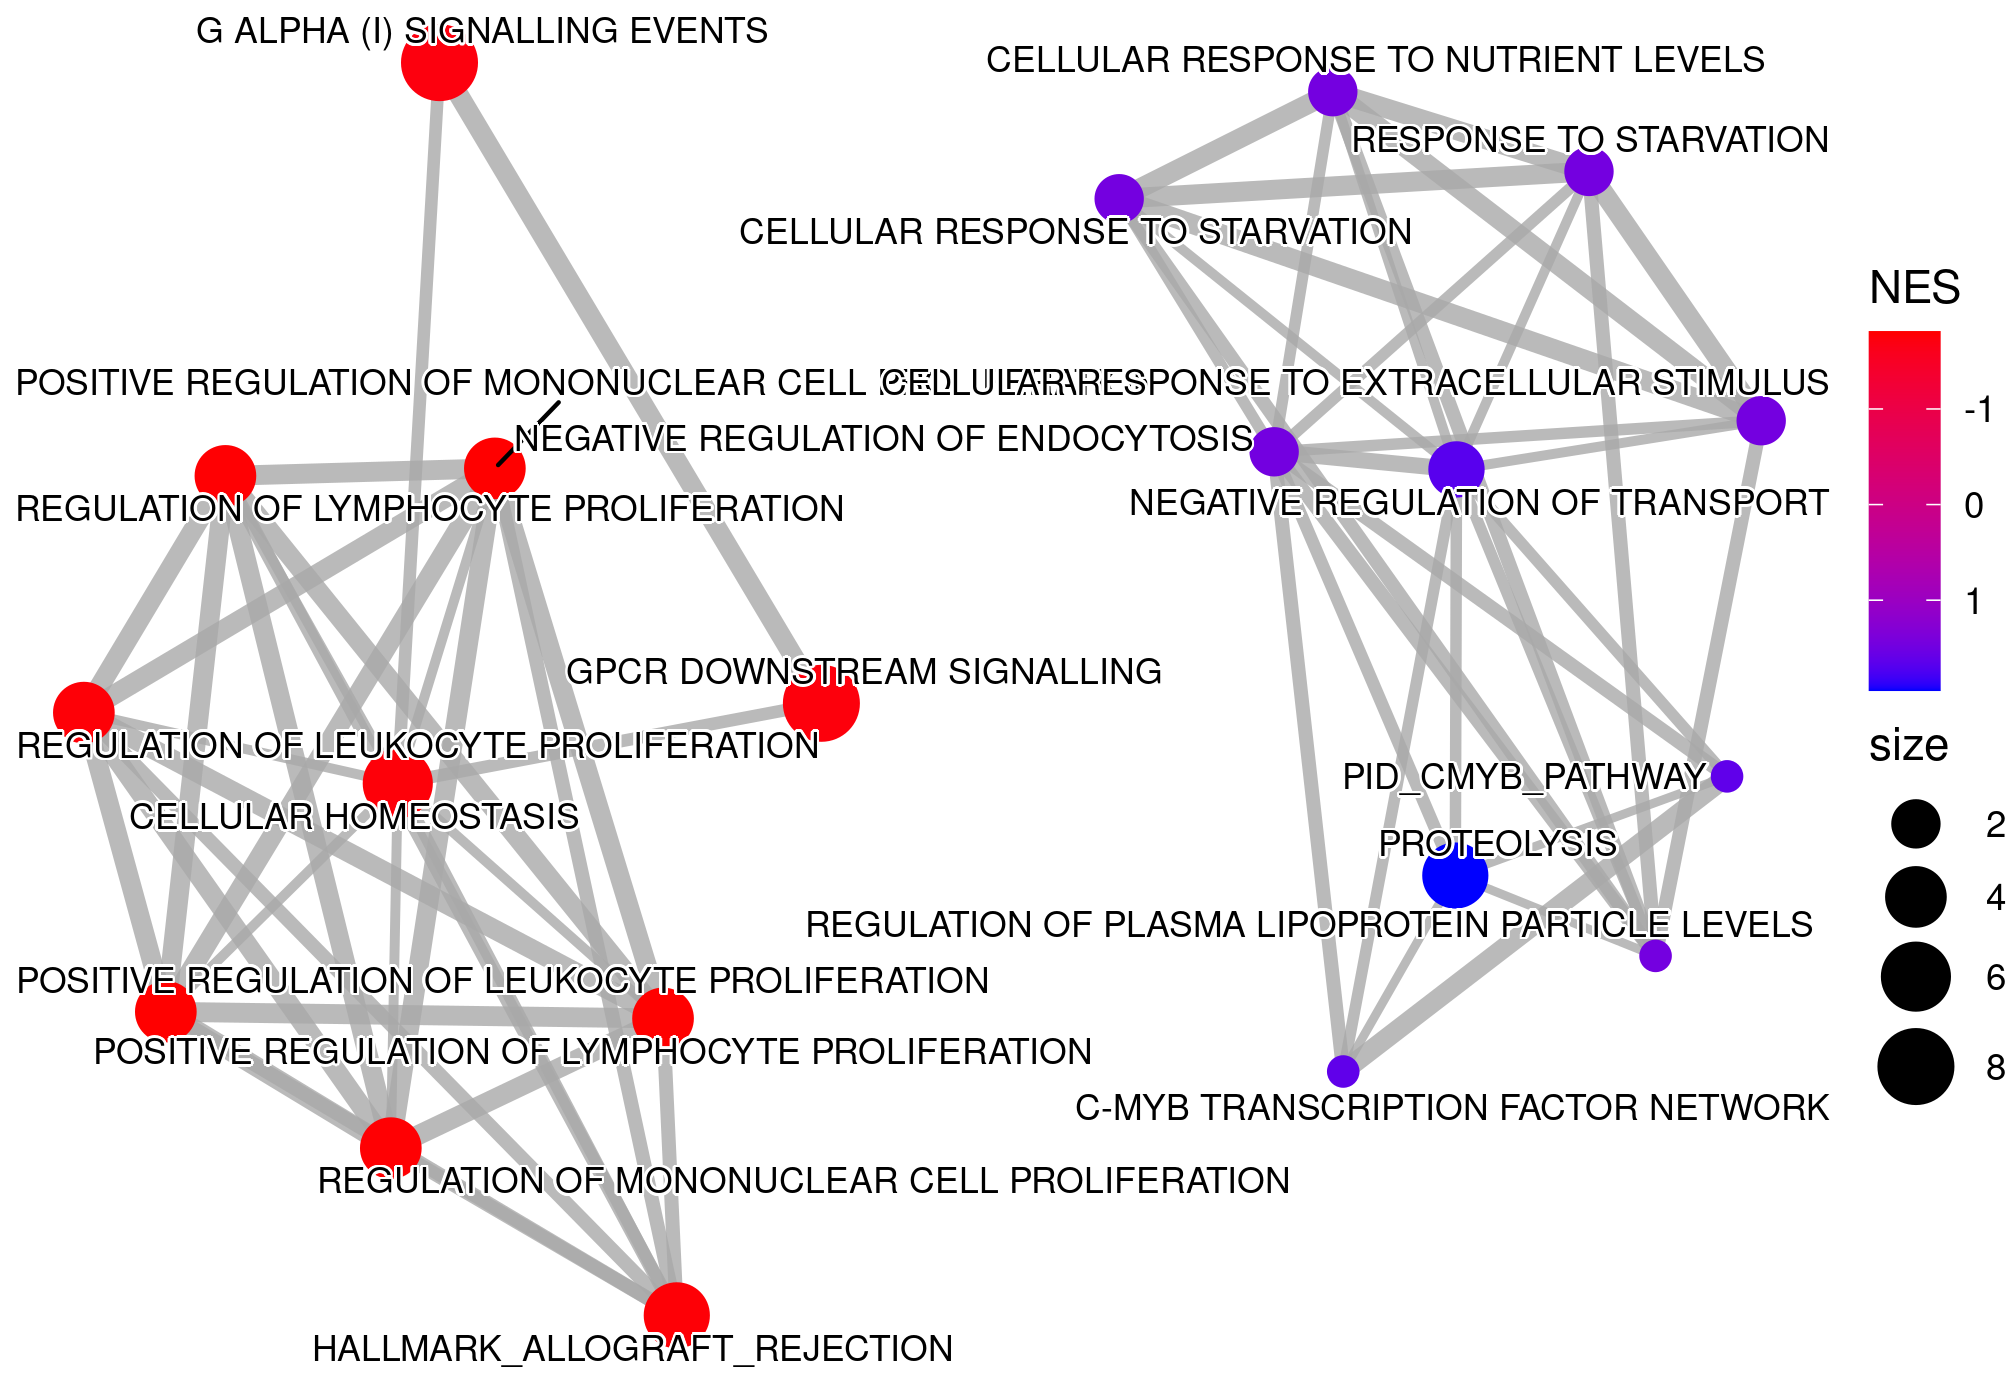
\includegraphics[width=0.49\linewidth]{../Results/Plasma/Cortisone/Cortisone_vs_No_Cortisone/Univariate/GSEA/Cortisone_vs_No_Cortisone_emap} 

}

\caption{Example of the different GSEA visualizations for cortisone versus no cortisone in Plasma. (Left)  Barplot of the gene sets with the 6 highest and 6 lowest NES values. (Right) Enrichment map of the 20 gene sets with the highest absolute NES values.}\label{fig:gseaPlotsCort}
\end{figure}

In addition, in the \textbf{Results/Plasma/Cortisone/Cortisone\_vs\_No\_Cortisone/Univariate/GSEA/GSEA\_PLOTS} and \textbf{Results/Serum/Cortisone/Cortisone\_vs\_No\_Cortisone/Univariate/GSEA/GSEA\_PLOTS}folder you can find a visualization of the location of the gene set genes in the ranked gene list and an ES calculation visualization (see Figure \ref{fig:gseaNesCort}).

\begin{figure}

{\centering 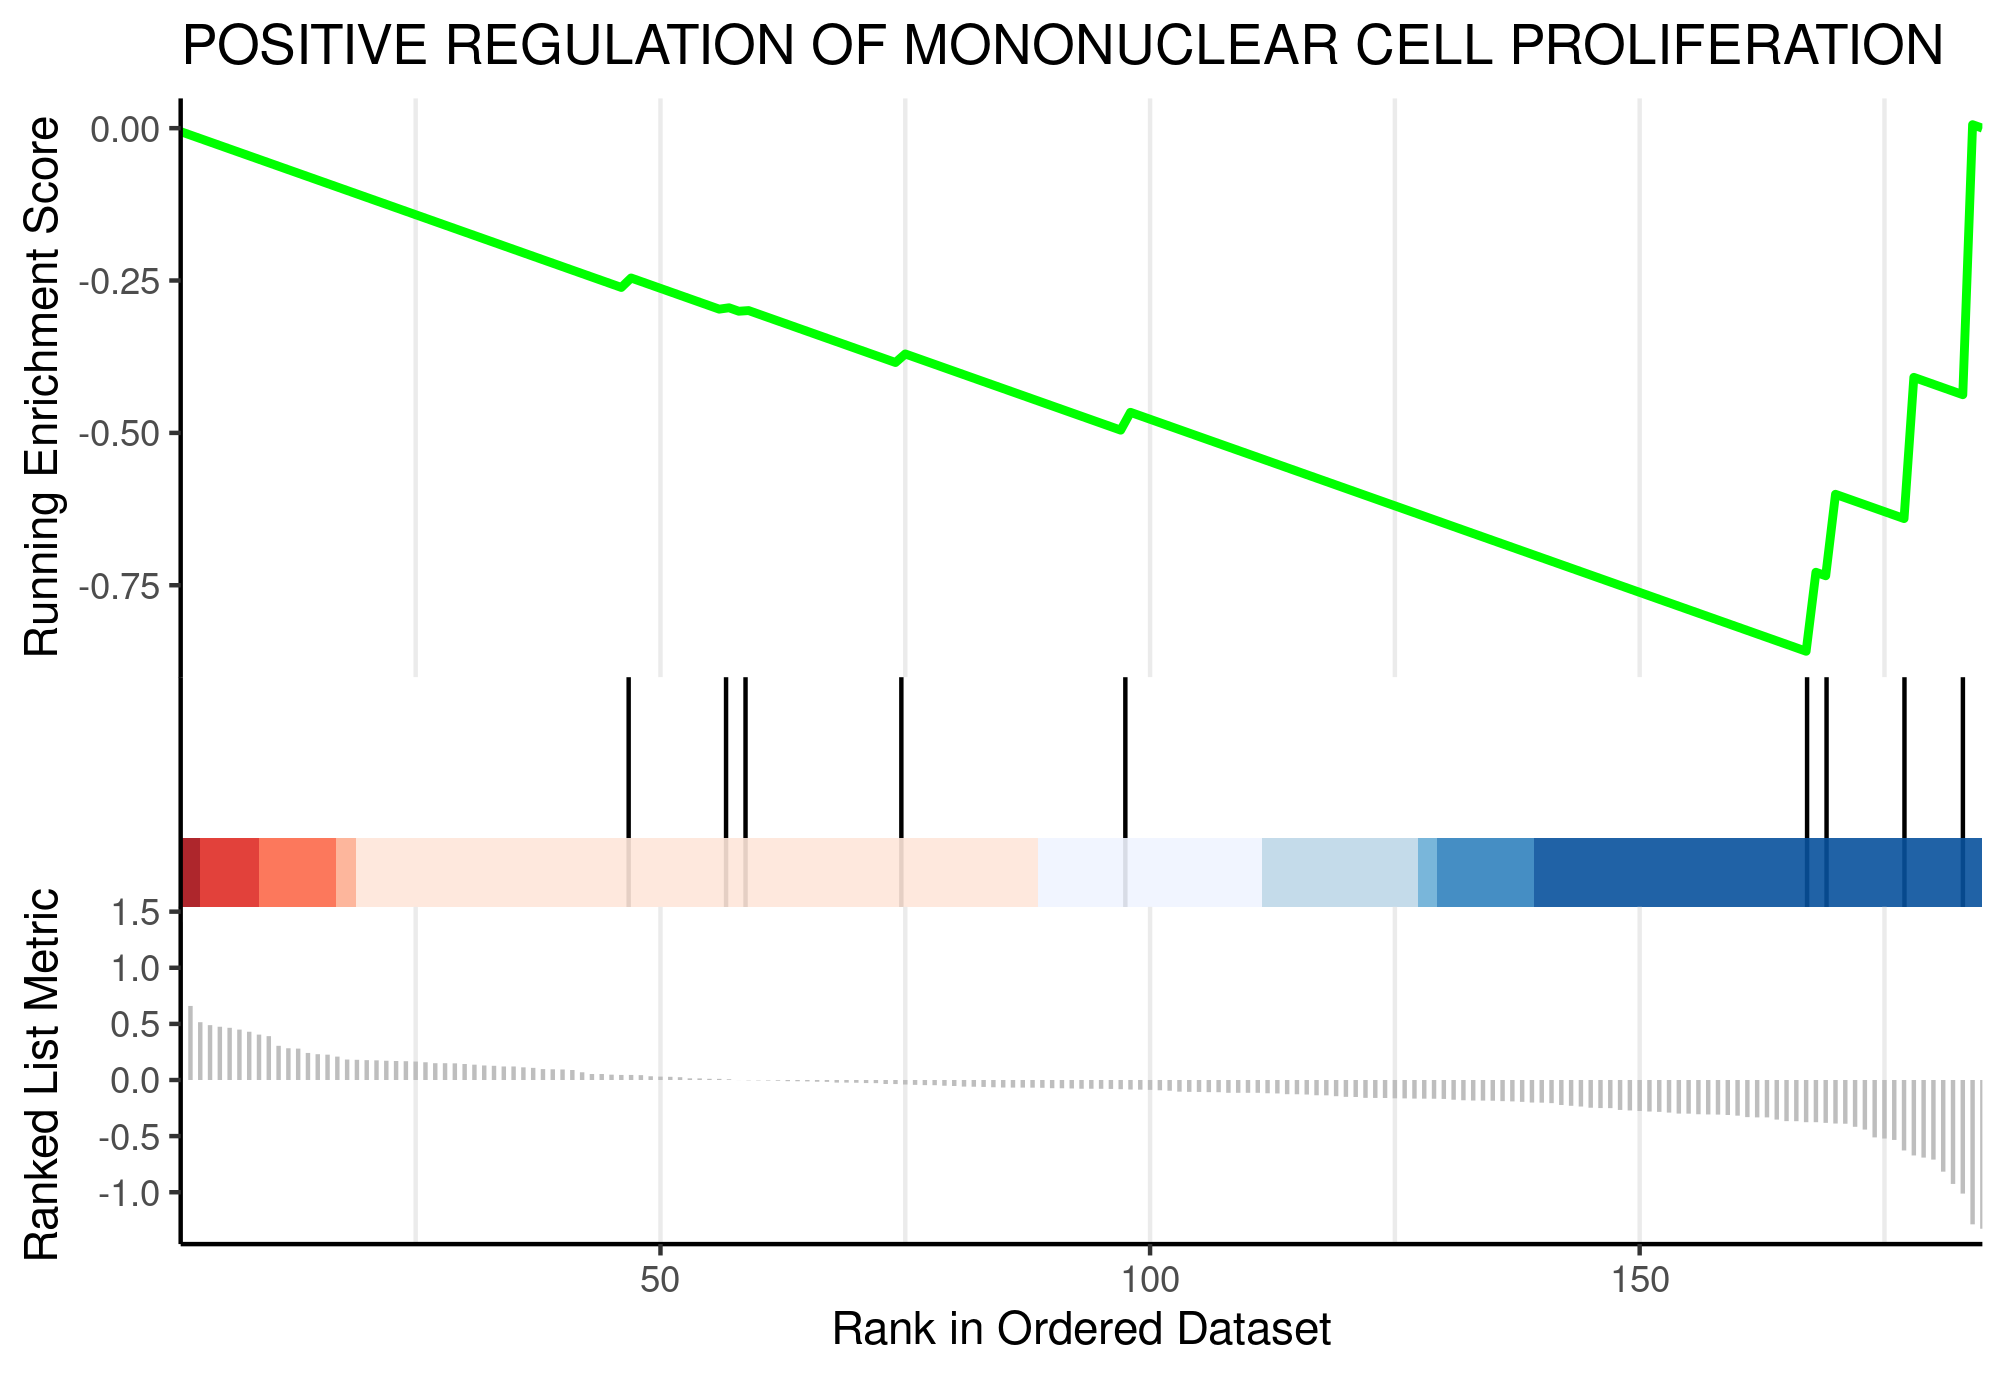
\includegraphics[width=0.49\linewidth]{../Results/Plasma/Cortisone/Cortisone_vs_No_Cortisone/Univariate/GSEA/GSEA_PLOTS/Cortisone_vs_No_Cortisone_gseaplot_POSITIVE_REGULA} 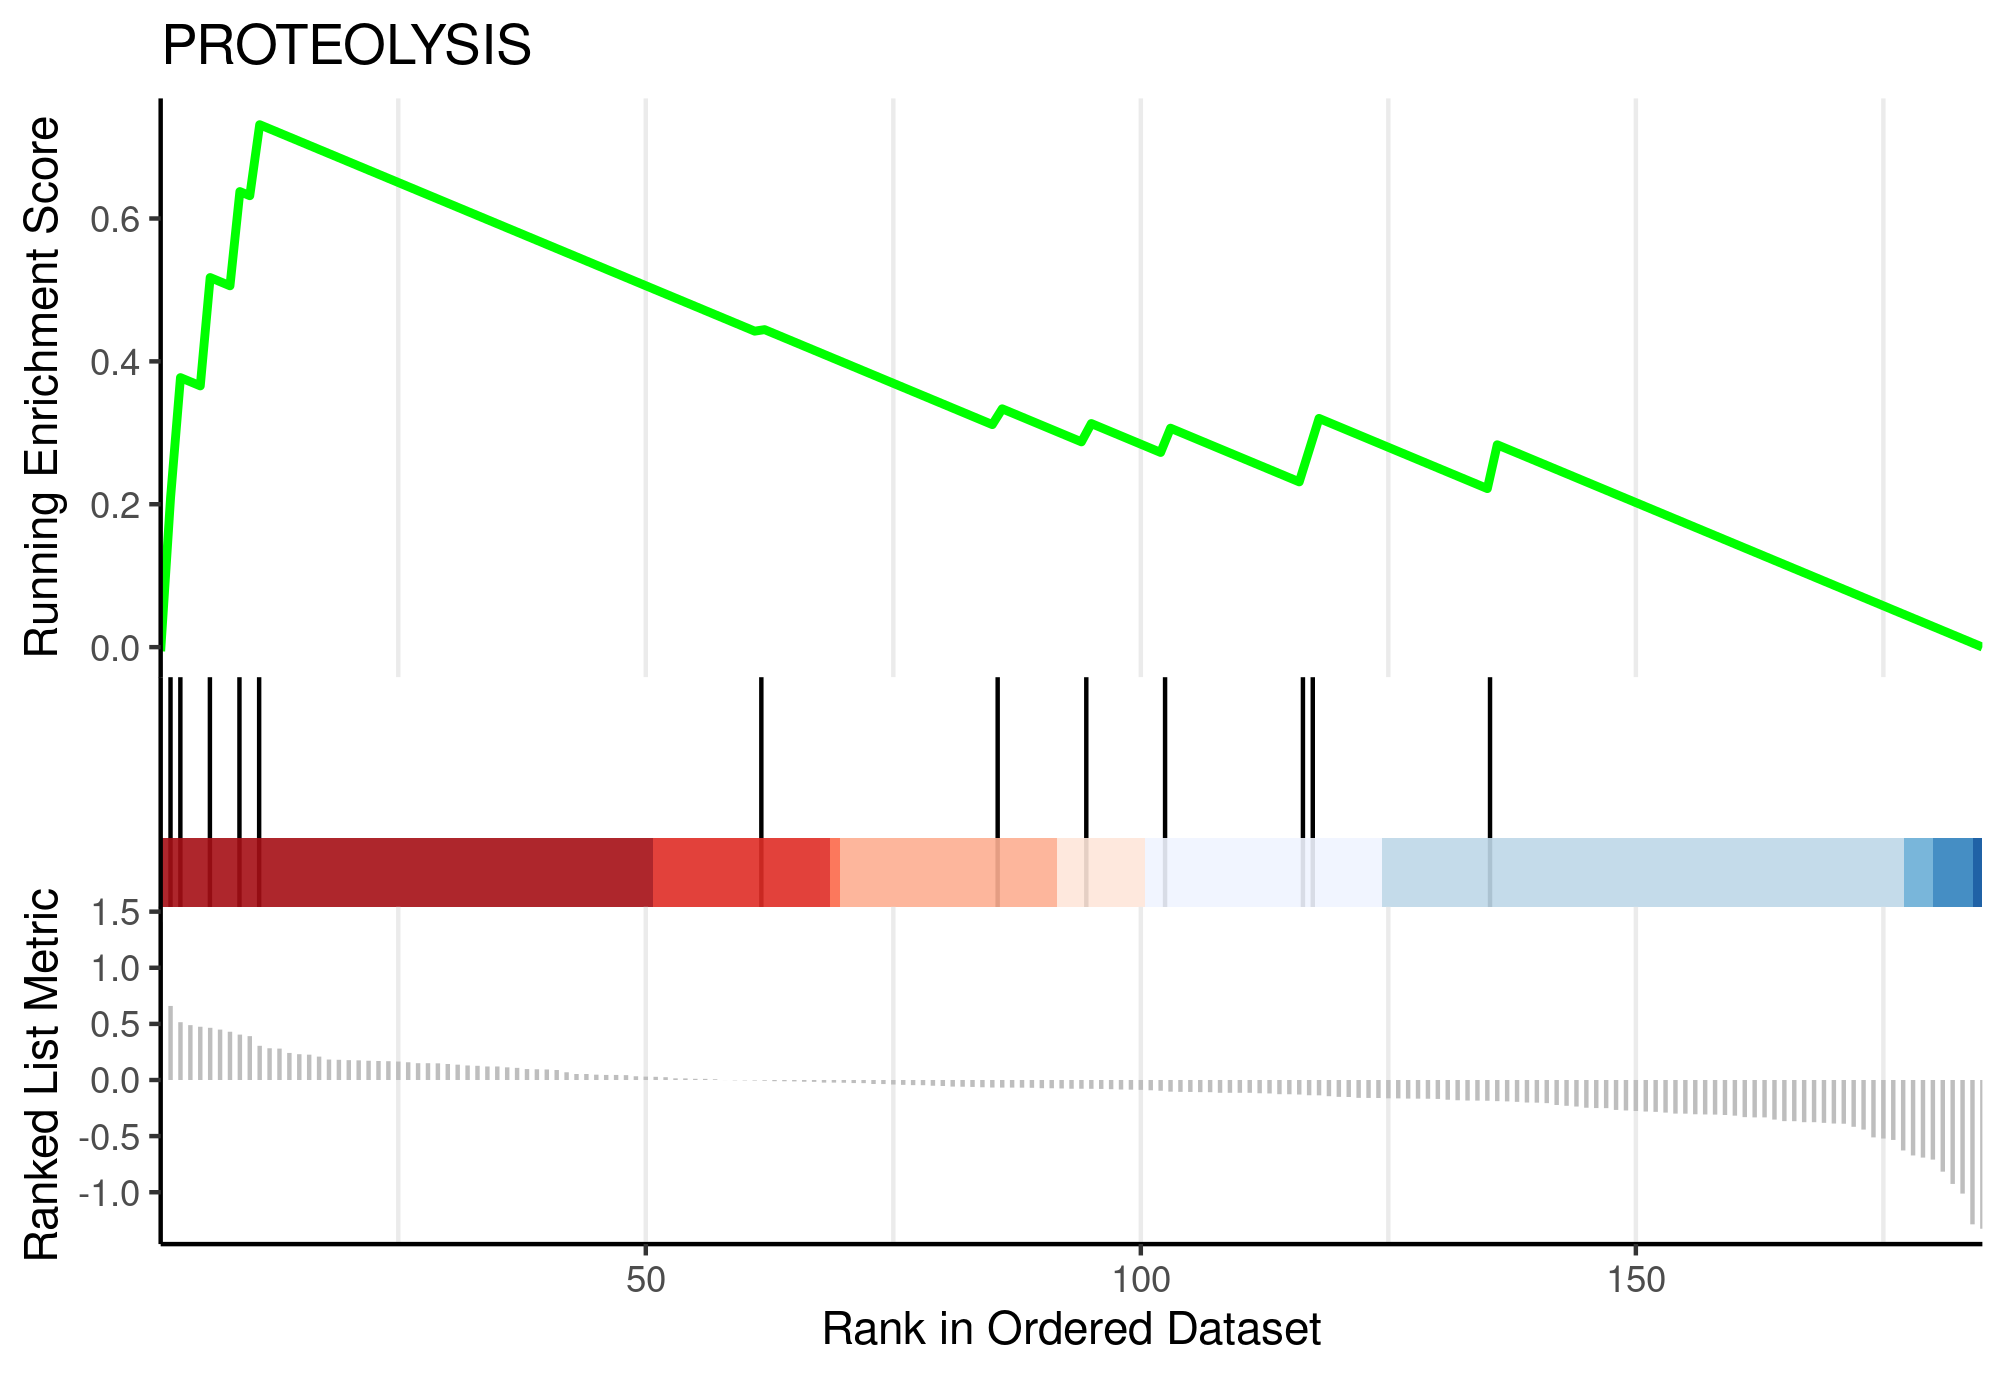
\includegraphics[width=0.49\linewidth]{../Results/Plasma/Cortisone/Cortisone_vs_No_Cortisone/Univariate/GSEA/GSEA_PLOTS/Cortisone_vs_No_Cortisone_gseaplot_PROTEOLYSIS} 

}

\caption{Example of two ES visualizations and calculation. (Left) Downregulation of cell proliferation. (Right) Upregulation of proteolysis.}\label{fig:gseaNesCort}
\end{figure}

\hypertarget{data-responsibility}{%
\chapter{Data Responsibility}\label{data-responsibility}}

\begin{itemize}
\tightlist
\item
  \textbf{NBIS \& Uppnex} Unfortunately, we do not have resources to keep any files associated with the support request. We suggest that you safely store the results delivered by us. In addition, we ask that you remove the files from UPPMAX/UPPNEX after analysis is completed. The main storage at UPPNEX is optimized for high-speed and parallel access, which makes it expensive and not the right place for long time archiving.
\item
  \textbf{Sensitive data} Please note that special considerations may apply to the human-derived sensitive personal data. These should be handled according to specific laws and regulations.
\item
  \textbf{Long-term backup} The responsibility for data archiving lies with universities and we recommend asking your local IT for support with long-term data archiving. Also the newly established Data Office at SciLifeLab may be of help to discuss other options.
\end{itemize}

\hypertarget{acknowledgements}{%
\chapter{Acknowledgements}\label{acknowledgements}}

If you are presenting the results in a paper, at a workshop or conference, we kindly ask you to acknowledge us.

\begin{itemize}
\item
  \textbf{NBIS Staff} are encouraged to be co-authors when this is merited in accordance to the ethical recommendations for authorship, e.g.~\texttt{ICMJE\ recommendations\ \textless{}http://www.icmje.org/recommendations/browse/roles-and-responsibilities/defining-the-role-of-authors-and-contributors.html\textgreater{}}\emph{). If applicable, please include \textbf{Vincent van Hoef, National Bioinformatics Infrastructure Sweden, Science for Life Laboratory, Uppsala University}, as co-author. In other cases, NBIS would be grateful if support by us is acknowledged in publications according to this example: \texttt{"Support\ by\ NBIS\ (National\ Bioinformatics\ Infrastructure\ Sweden)\ is\ gratefully\ acknowledged"\ \ \ \textless{}https://www.nbis.se/resources/support.html\textgreater{}}}.
\item
  \textbf{UPPMAX} If your project has used HPC resources we kindly asks you to acknowledge UPPMAX and SNIC. If applicable, please add: \texttt{"The\ computations\ were\ performed\ on\ resources\ provided\ by\ SNIC\ through\ Uppsala\ Multidisciplinary\ Center\ for\ Advanced\ Computational\ Science\ (UPPMAX)\ under\ Project\ SNIC\ XXXX/Y-ZZZ"\ \ \ \textless{}https://www.uppmax.uu.se/support/faq/general-miscellaneous-faq/acknowledging-uppmax-\/-snic-\/-and-uppnex/\textgreater{}}\_.
\item
  \textbf{NGI} In publications based on data from NGI Sweden, the authors must acknowledge SciLifeLab, NGI and UPPMAX: \texttt{"The\ authors\ would\ like\ to\ acknowledge\ support\ from\ Science\ for\ Life\ Laboratory,\ the\ National\ Genomics\ Infrastructure,\ NGI,\ and\ Uppmax\ for\ providing\ assistance\ in\ massive\ parallel\ sequencing\ and\ computational\ infrastructure"\ \textless{}https://ngisweden.scilifelab.se/info/faq\#how-do-i-acknowledge-ngi-in-my-publication\textgreater{}}\_.
\end{itemize}

\hypertarget{closing-procedures}{%
\chapter{Closing Procedures}\label{closing-procedures}}

You should soon be contacted by one of our managers, \href{jessica.lindvall@nbis.se}{Jessica Lindvall} or \href{henrik.lantz@nbis.se}{Henrik Lantz}, with a request to close down the project in our internal system and for invoicing matters. If we do not hear from you within \textbf{30 days} the project will be automatically closed and invoice sent. Again, we would like to remind you about data responsibility and acknowledgements, see Data Responsibility and Acknowledgments sections.

You are naturally more than welcome to come back to us with further data analysis request at any time via \href{http://nbis.se/support/support.html}{NBIS support}.

Thank you for using NBIS and all the best for future research.

\end{document}
